\documentclass[a4paper, 10pt]{article}
\usepackage[top=60pt,bottom=60pt,left=90pt,right=90pt]{geometry}
\usepackage[utf8]{inputenc}

\usepackage{hyperref}
\usepackage{siunitx}
\usepackage{graphicx}
\usepackage{float}
\usepackage{subcaption}
\usepackage{cleveref}
\usepackage{listings}
\usepackage{pdfpages}
\usepackage[toc,page]{appendix}

\renewcommand{\fancyrefdefaultformat}{plain}

\title{xPIN Diode + Sample and Hold + NI-6002 Manual}
% \author{Jan Kočka}

\begin{document}

\maketitle

\vspace*{15em}

\tableofcontents

\vspace{15em}

\section{Introduction}
This manual describes the usage of the PIN diode + Sample and Hold () + NI-6002 setup in ELI Beamlines, which is used for shot to shot x-ray photon pulse detection at the PXS experiment in E1.
This section will provide a brief overview of the theory around it.
In the next section all the separate parts will be described in more detail and instructions on how to connect them together will follow.

The advantages of the PIN diode in those scenarios is that it has a sufficient time resolution and that it is mainly sensitive to photons up to a certain energy.
That reduces the overall photon count which in turn increases the accuracy.
To get the full experimental setup we also need an oscilloscope and a trigger signal synchronised with the pulses.
To use the S\&H we also need a way to delay the trigger by an adjustable amount, for that we use a signal generator in the "triggered" mode.
The last thing we need is the NI-6002 device and a computer with the software for it instaled.

% That means that the diode can more accurately capture the photon count as there is less over overall photons and you can also be certain they are in the range you want.

In short a PIN diode is a P-N junction but with a section of undoped (Intrinsic) semiconductor between the P and N regions.
The diode is reverse biased and when a photon hits the intrinsic zone it knocks an electron out of its place.
The electron-hole pair that was created is then split by the voltage over the region and creates a current.
This current however is usually very small and needs to be amplified.
% Earlier I wrote that the PIN diode is mainly sensitive to photons up to a certain energy.
% This cutoff energy is determined by the thickness of the diode, the thicker diode the more sensitive it will be to high energy photons.

\begin{figure}[h]
    \centering
    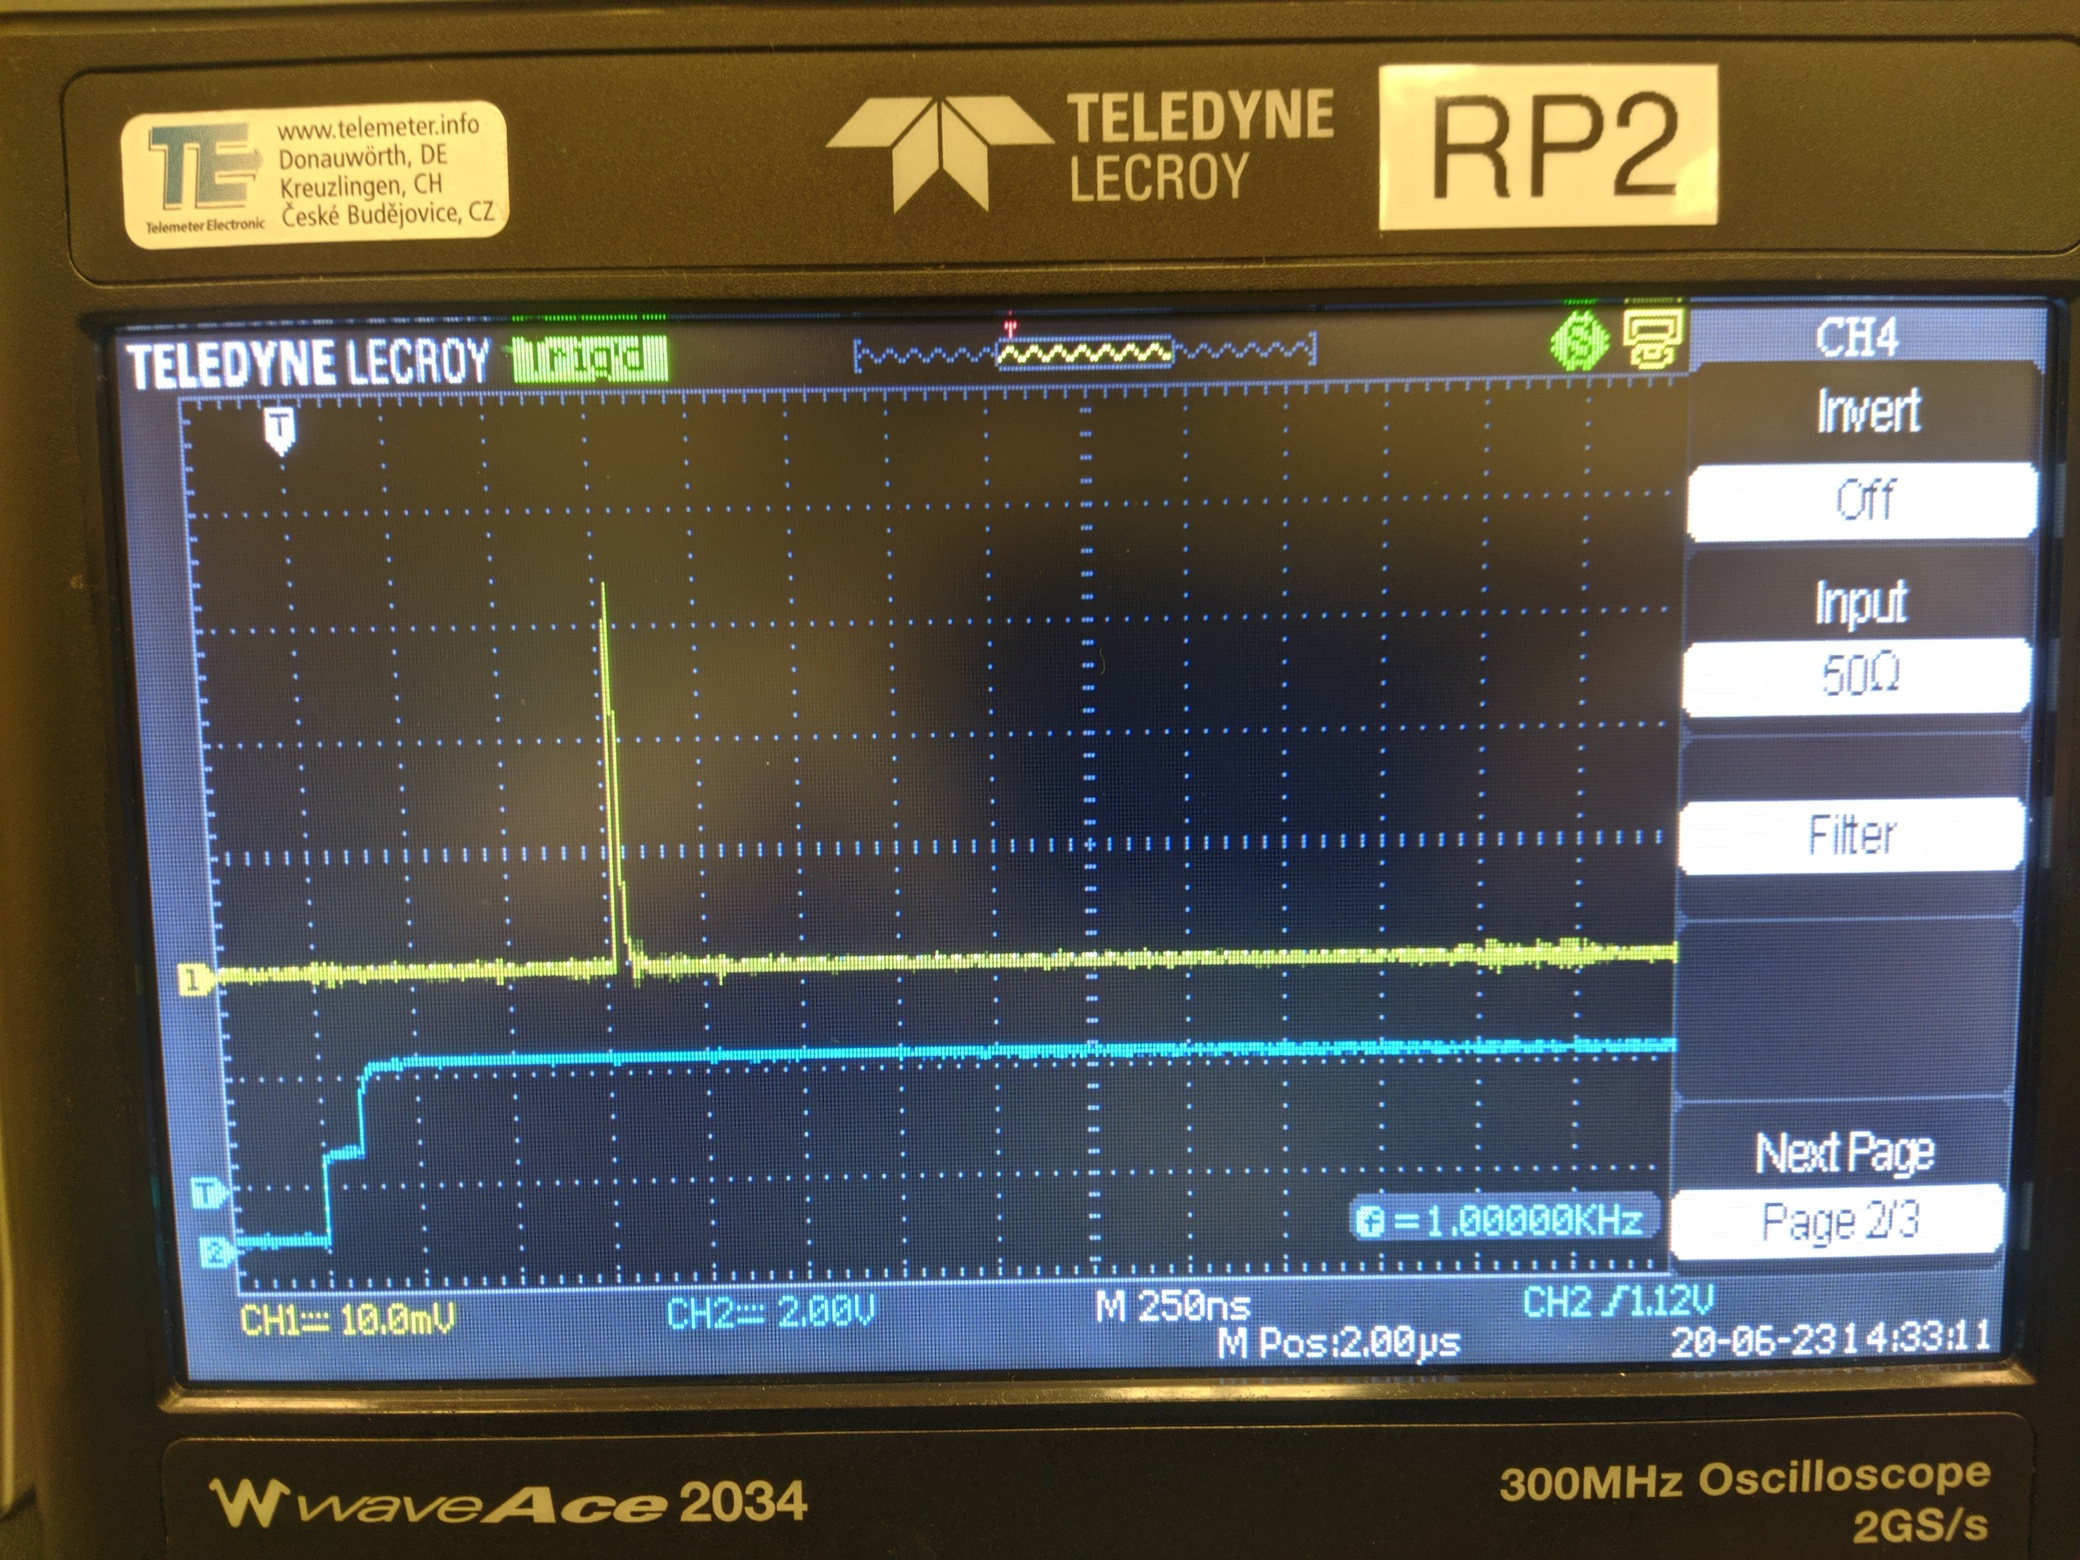
\includegraphics[width=0.9\textwidth]{./images/pulse-shape.jpg}
    \caption{The shape of the PIN output signal (yellow line) viewed by an oscilloscope}
    \label{fig:pulse-shape}
\end{figure}

It was mentioned that the time resolution of the PIN diode is very good, however that means that the measured signal can also get very short.
In our lab the photon pulse is around 20 \si{\femto\second} and the pulse that comes from the diode can be about 70 \si{\nano\second}.
In order to estimate the number of photons per pulse we need to get the area of the pulse.
Since the shape of the measured pulse (shown in \cref{fig:pulse-shape}) is quite constant, we decided that instead of using an expensive data acquisition device that could capture the nanosecond range pulse accurately we would use the S\&H.
The S\&H is a device which captures the signal it gets and holds it for a specified amount of time.
This lets us get the height of the pulse peak and hold it until the next pulse, which makes it much easier to capture.
Specifically in our lab the pulse frequency is 1 \si{\kilo\hertz}, that means that we can hold the peak hight for half a microsecond, this way even a 4 \si{\kilo\hertz} data acquisition device should provide accurate data.
This signal is then captured by the NI-6002 and analysed by the computer connected to it.


\section{Parts}
This parts introduces the specific parts we are using.

\subsection{PIN Diode}
We are using an xPIN diode from RIGAKU, the product page on their website can be found \href{https://www.rigaku.com/products/detectors/xpin}{here} \footnote{https://www.rigaku.com/products/detectors/xpin}.
However the bias box shown there is different from the one we are currently using.
Its spectral range is 5 \si{\kilo\electronvolt} (T = 10\%) – 27 \si{\kilo\electronvolt} (above 10\% of peak sensitivity).
The bias box we have provides a reverse bias of 50 \si{\volt} and amplifies the signal from the diode.

The device has 3 parts: the PIN diode itself, the bias box and a cable connecting the two (\cref{fig:pin-parts}).
The bias box has two more connections: a micro USB power cable and a BNC connection for the output signal.
For the micro USB power source, we used a small battery as it provides a more stable output then other sources we had available.
A picture of the diode setup can be seen in \cref{fig:pin-setup}.

The PIN diode is simple to setup as it has no adjustable settings, just connect all the parts together and get the output.

\begin{figure}[h]
    \centering
    \begin{subfigure}{0.4\textwidth}
        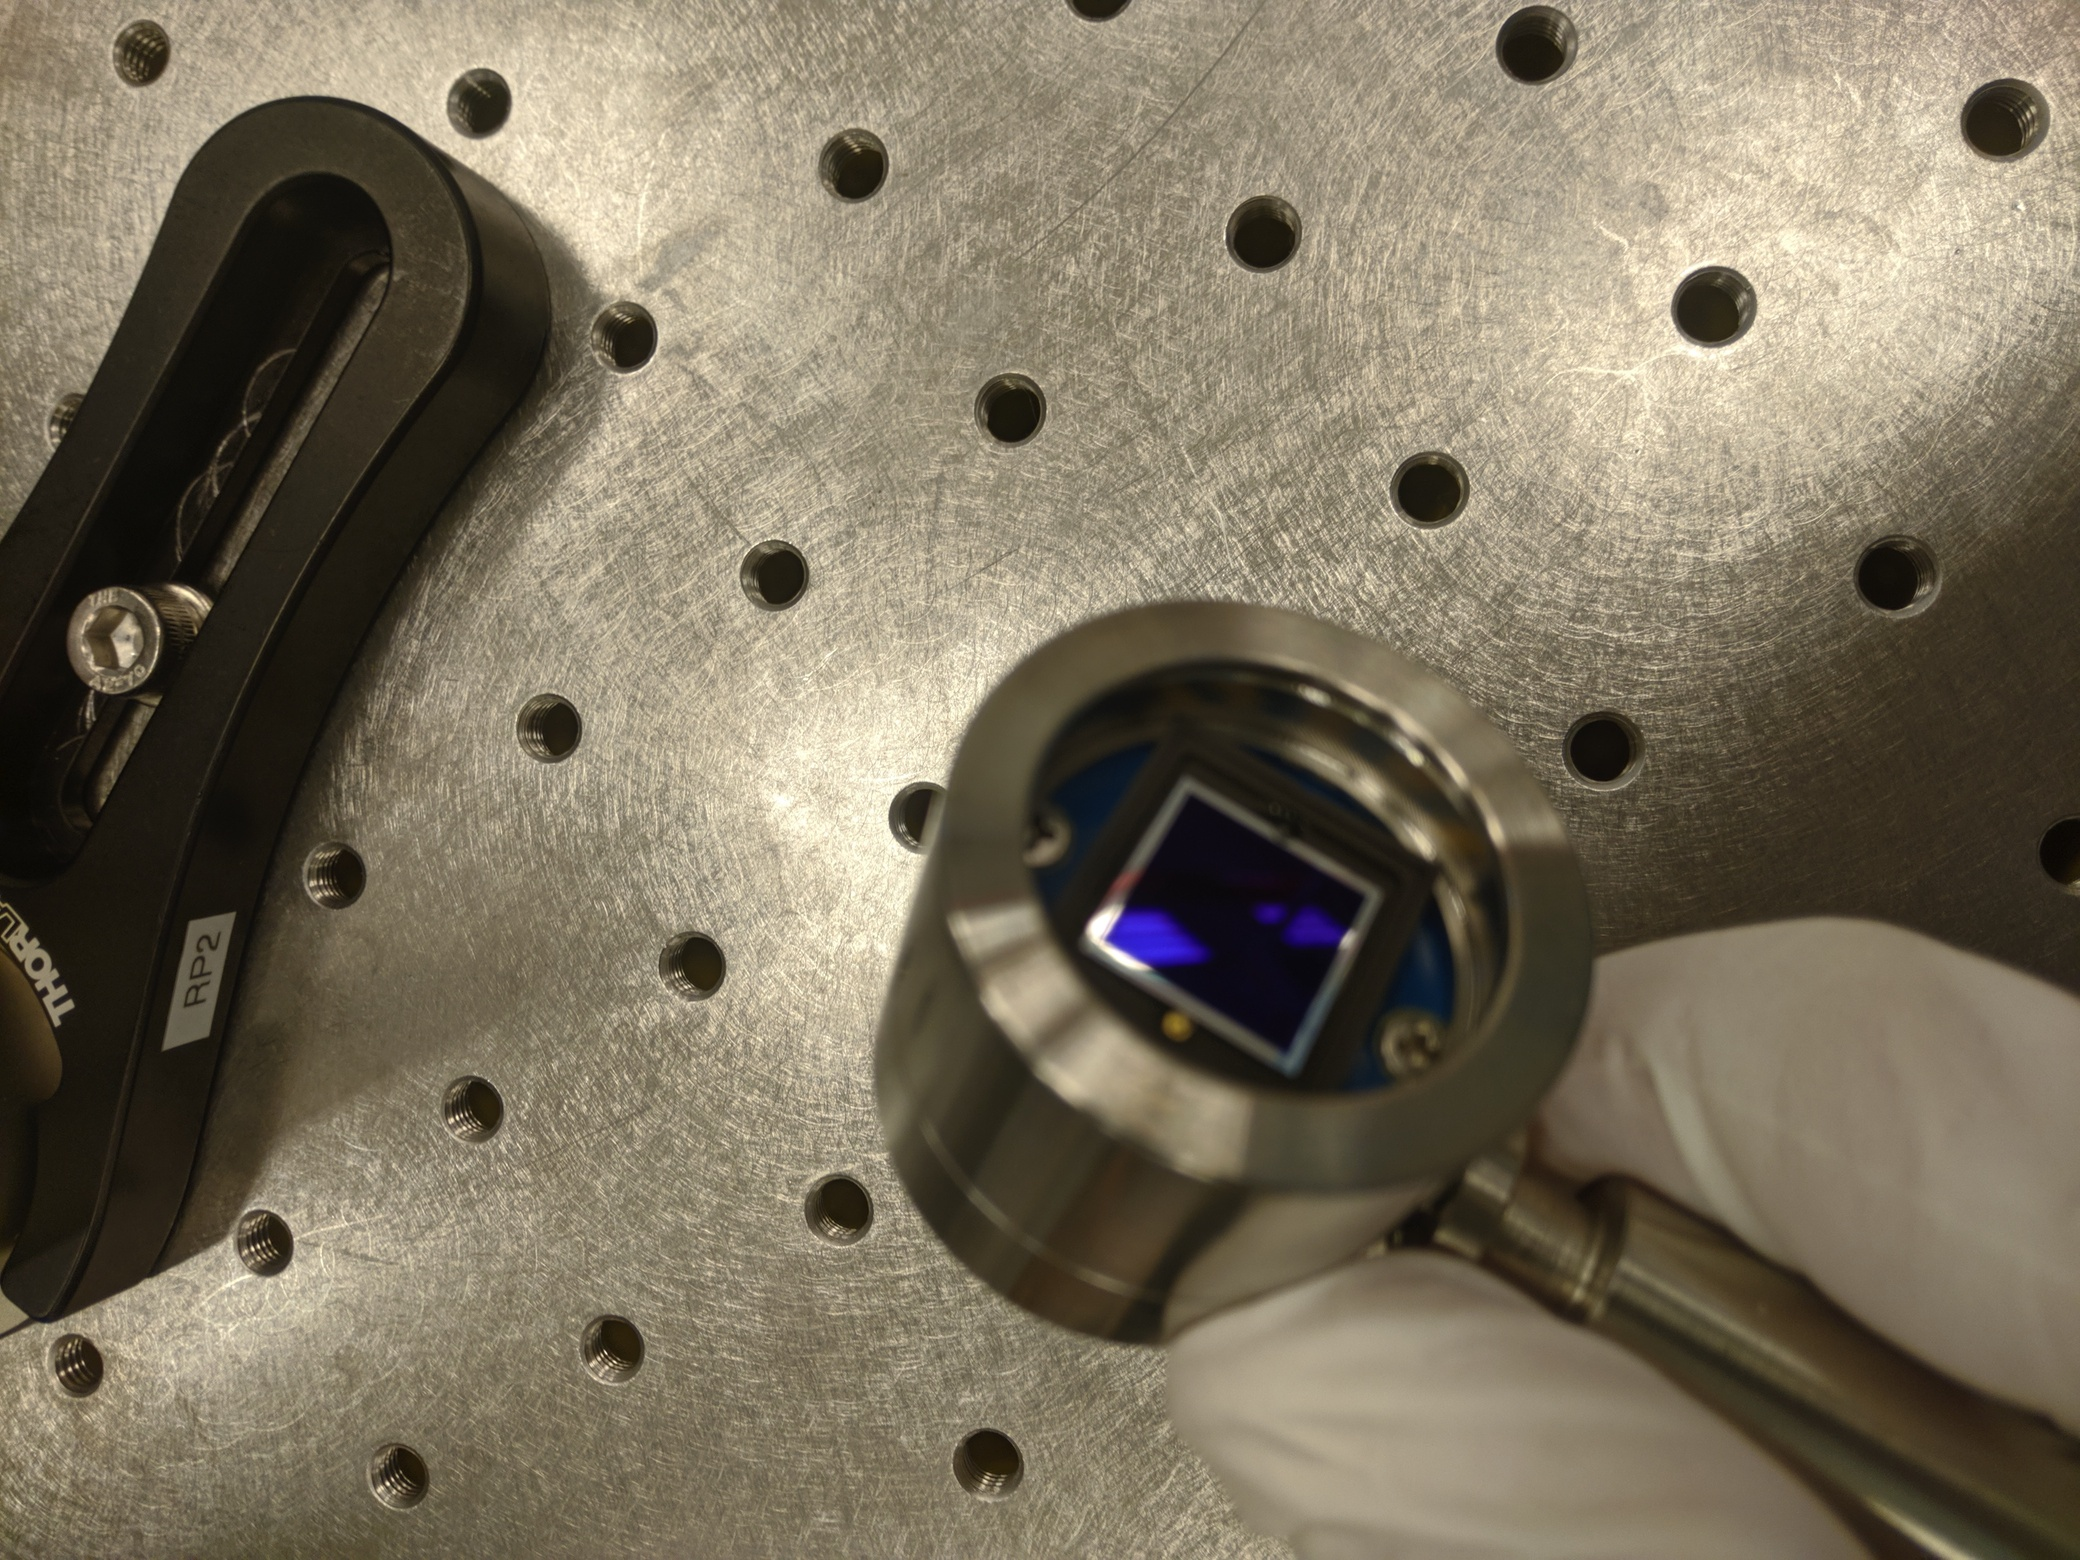
\includegraphics[width=\textwidth]{./images/pin-front.jpg}
        \caption{The PIN diode, front view without VIS protection}
        \label{fig:pin-diode}
    \end{subfigure}
    \begin{subfigure}{0.4\textwidth}
        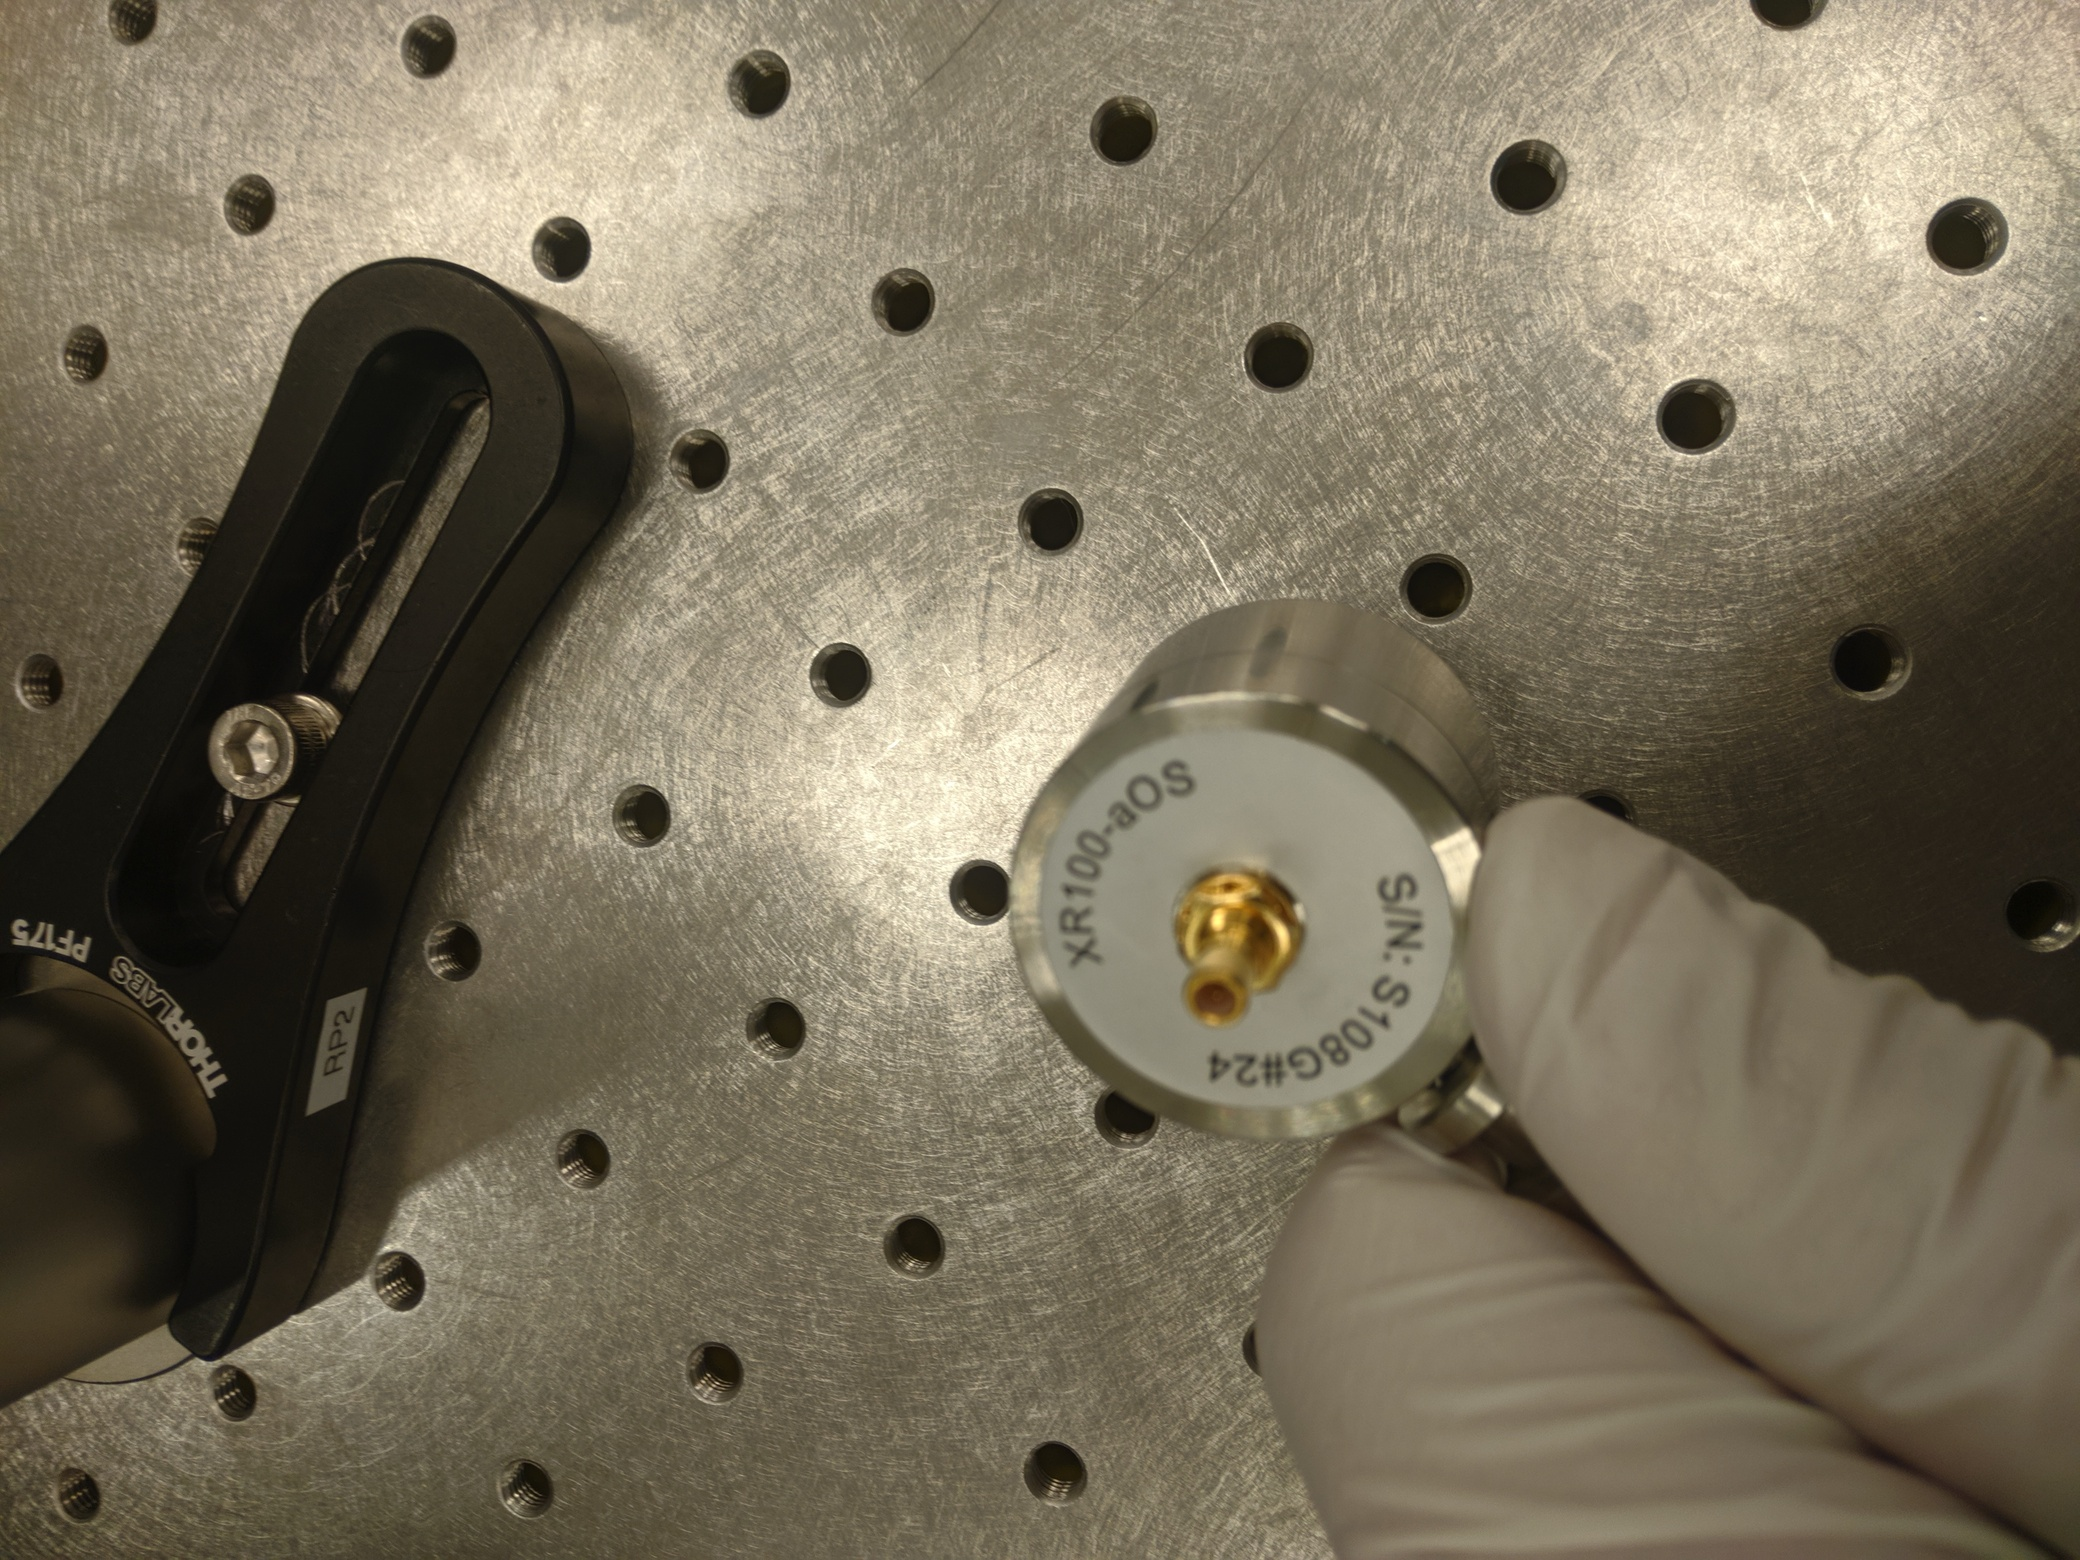
\includegraphics[width=\textwidth]{./images/pin-back.jpg}
        \caption{The PIN diode, back view}
        \label{fig:pin-diode}
    \end{subfigure}
    \begin{subfigure}{0.4\textwidth}
        \centering
        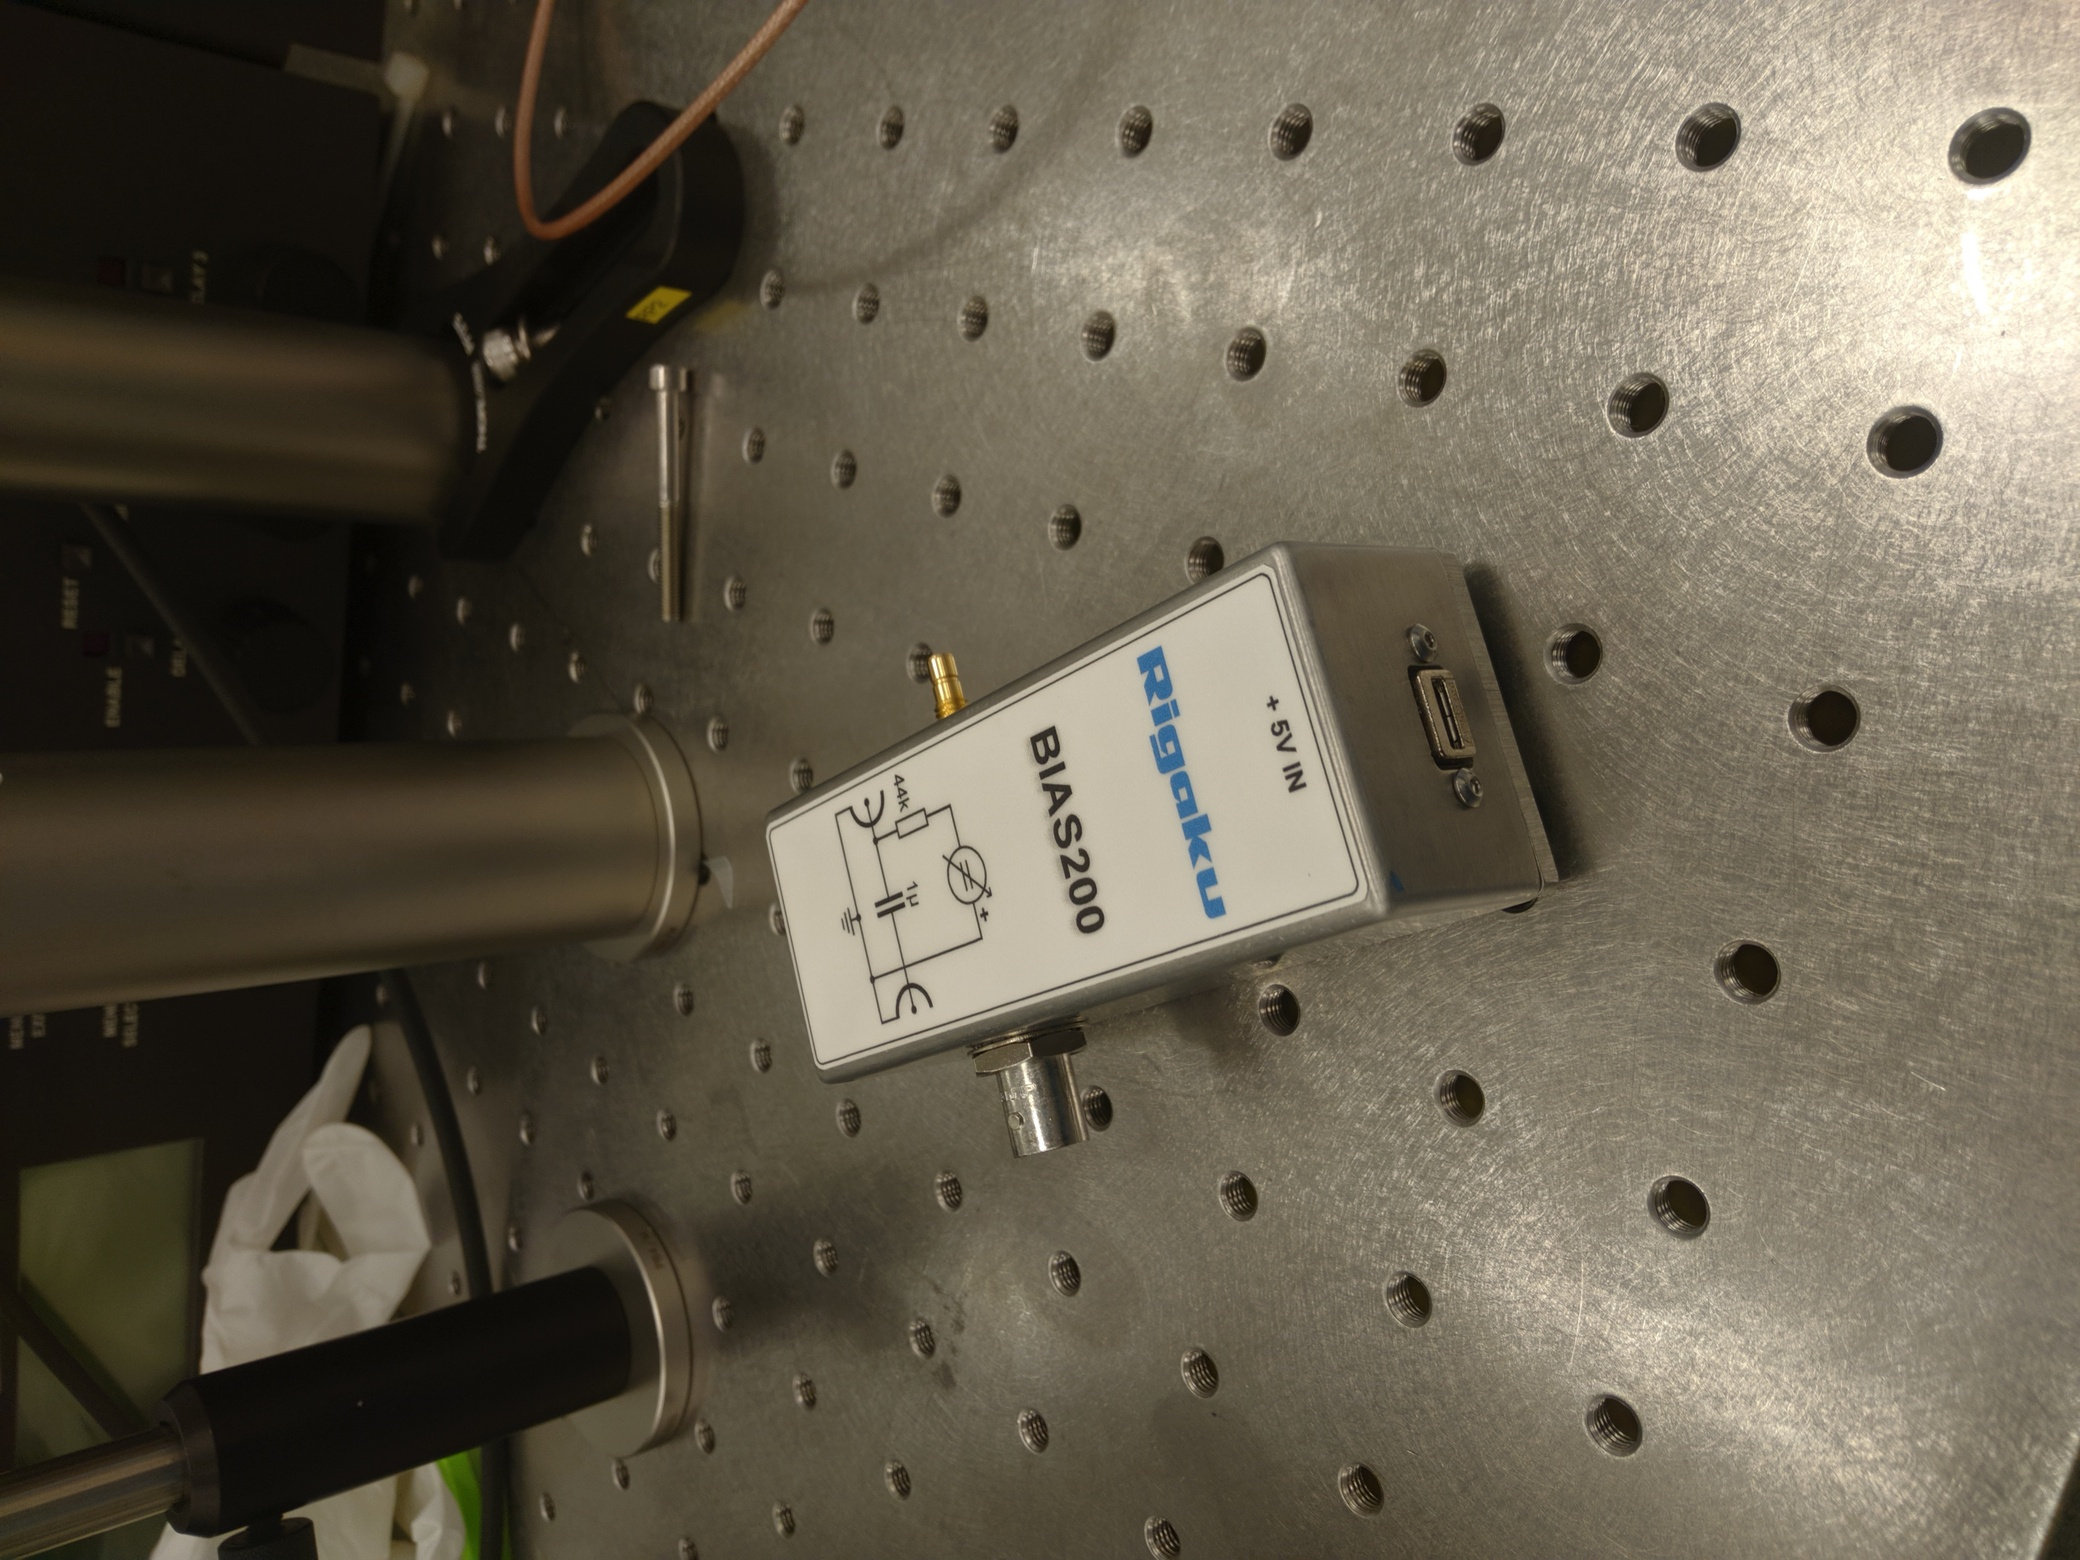
\includegraphics[width=\textwidth,angle=-90]{./images/pin-bias-box.jpg}
        \caption{The bias box}
        \label{fig:pin-diode}
    \end{subfigure}
    \begin{subfigure}{0.4\textwidth}
        \centering
        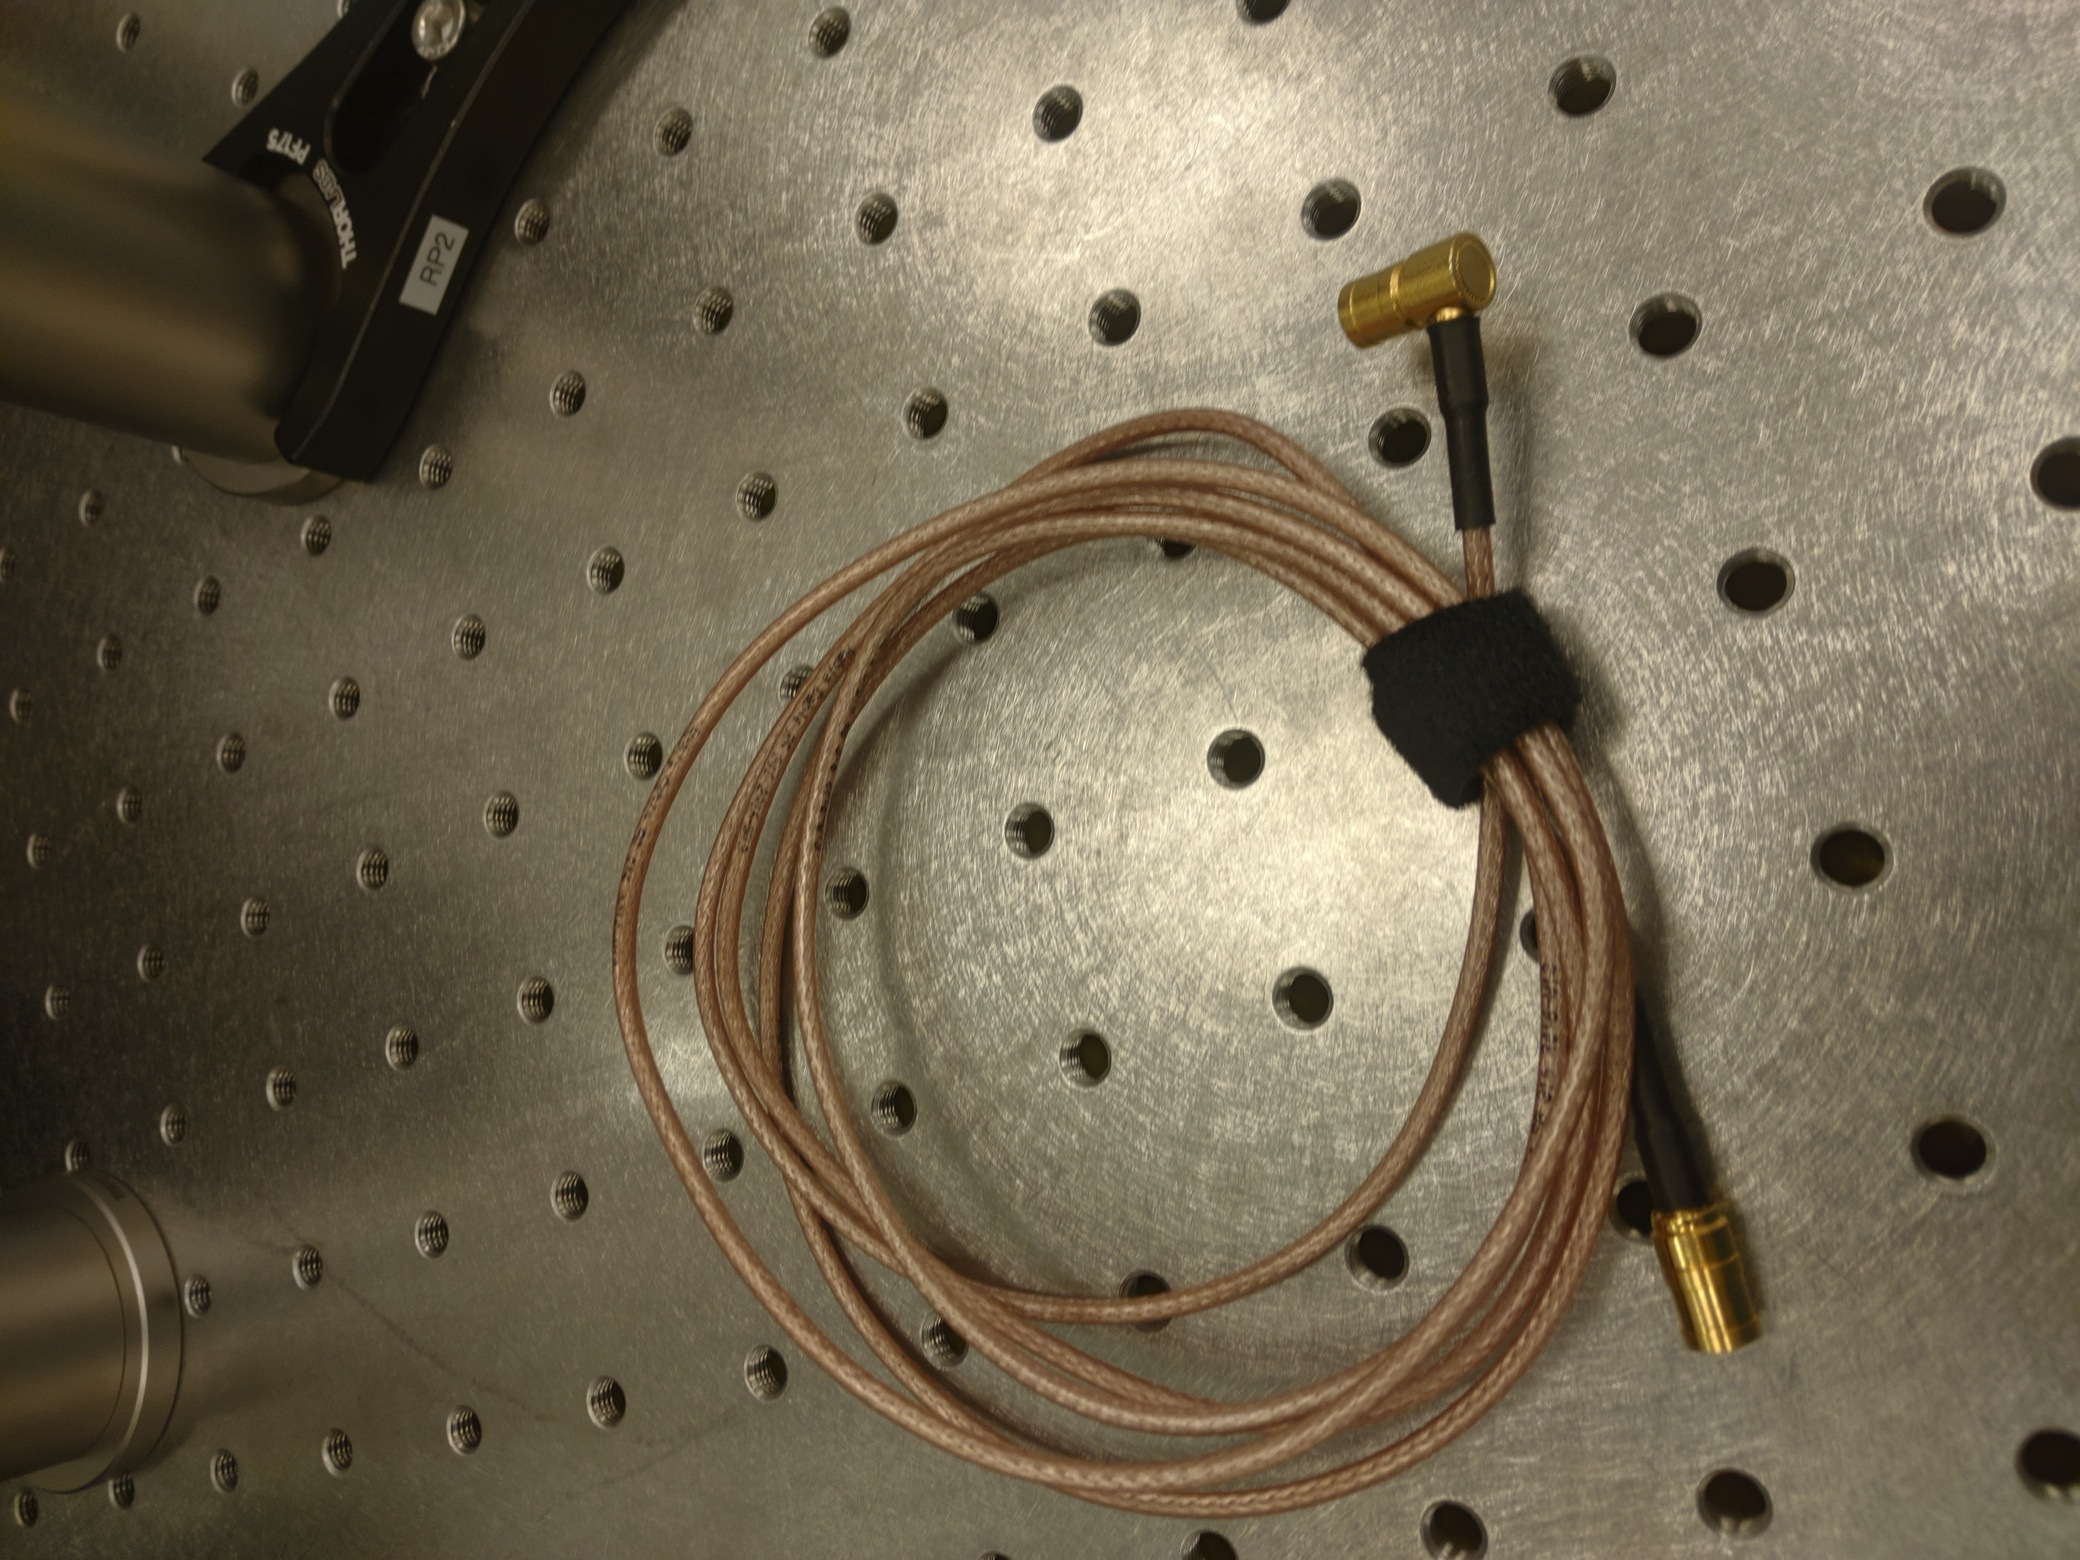
\includegraphics[width=\textwidth,angle=-90]{./images/pin-cable.jpg}
        \caption{The cable to connect them}
        \label{fig:pin-diode}
    \end{subfigure}
    \caption{PIN diode parts}
    \label{fig:pin-parts}
\end{figure}

\begin{figure}[H]
    \centering
    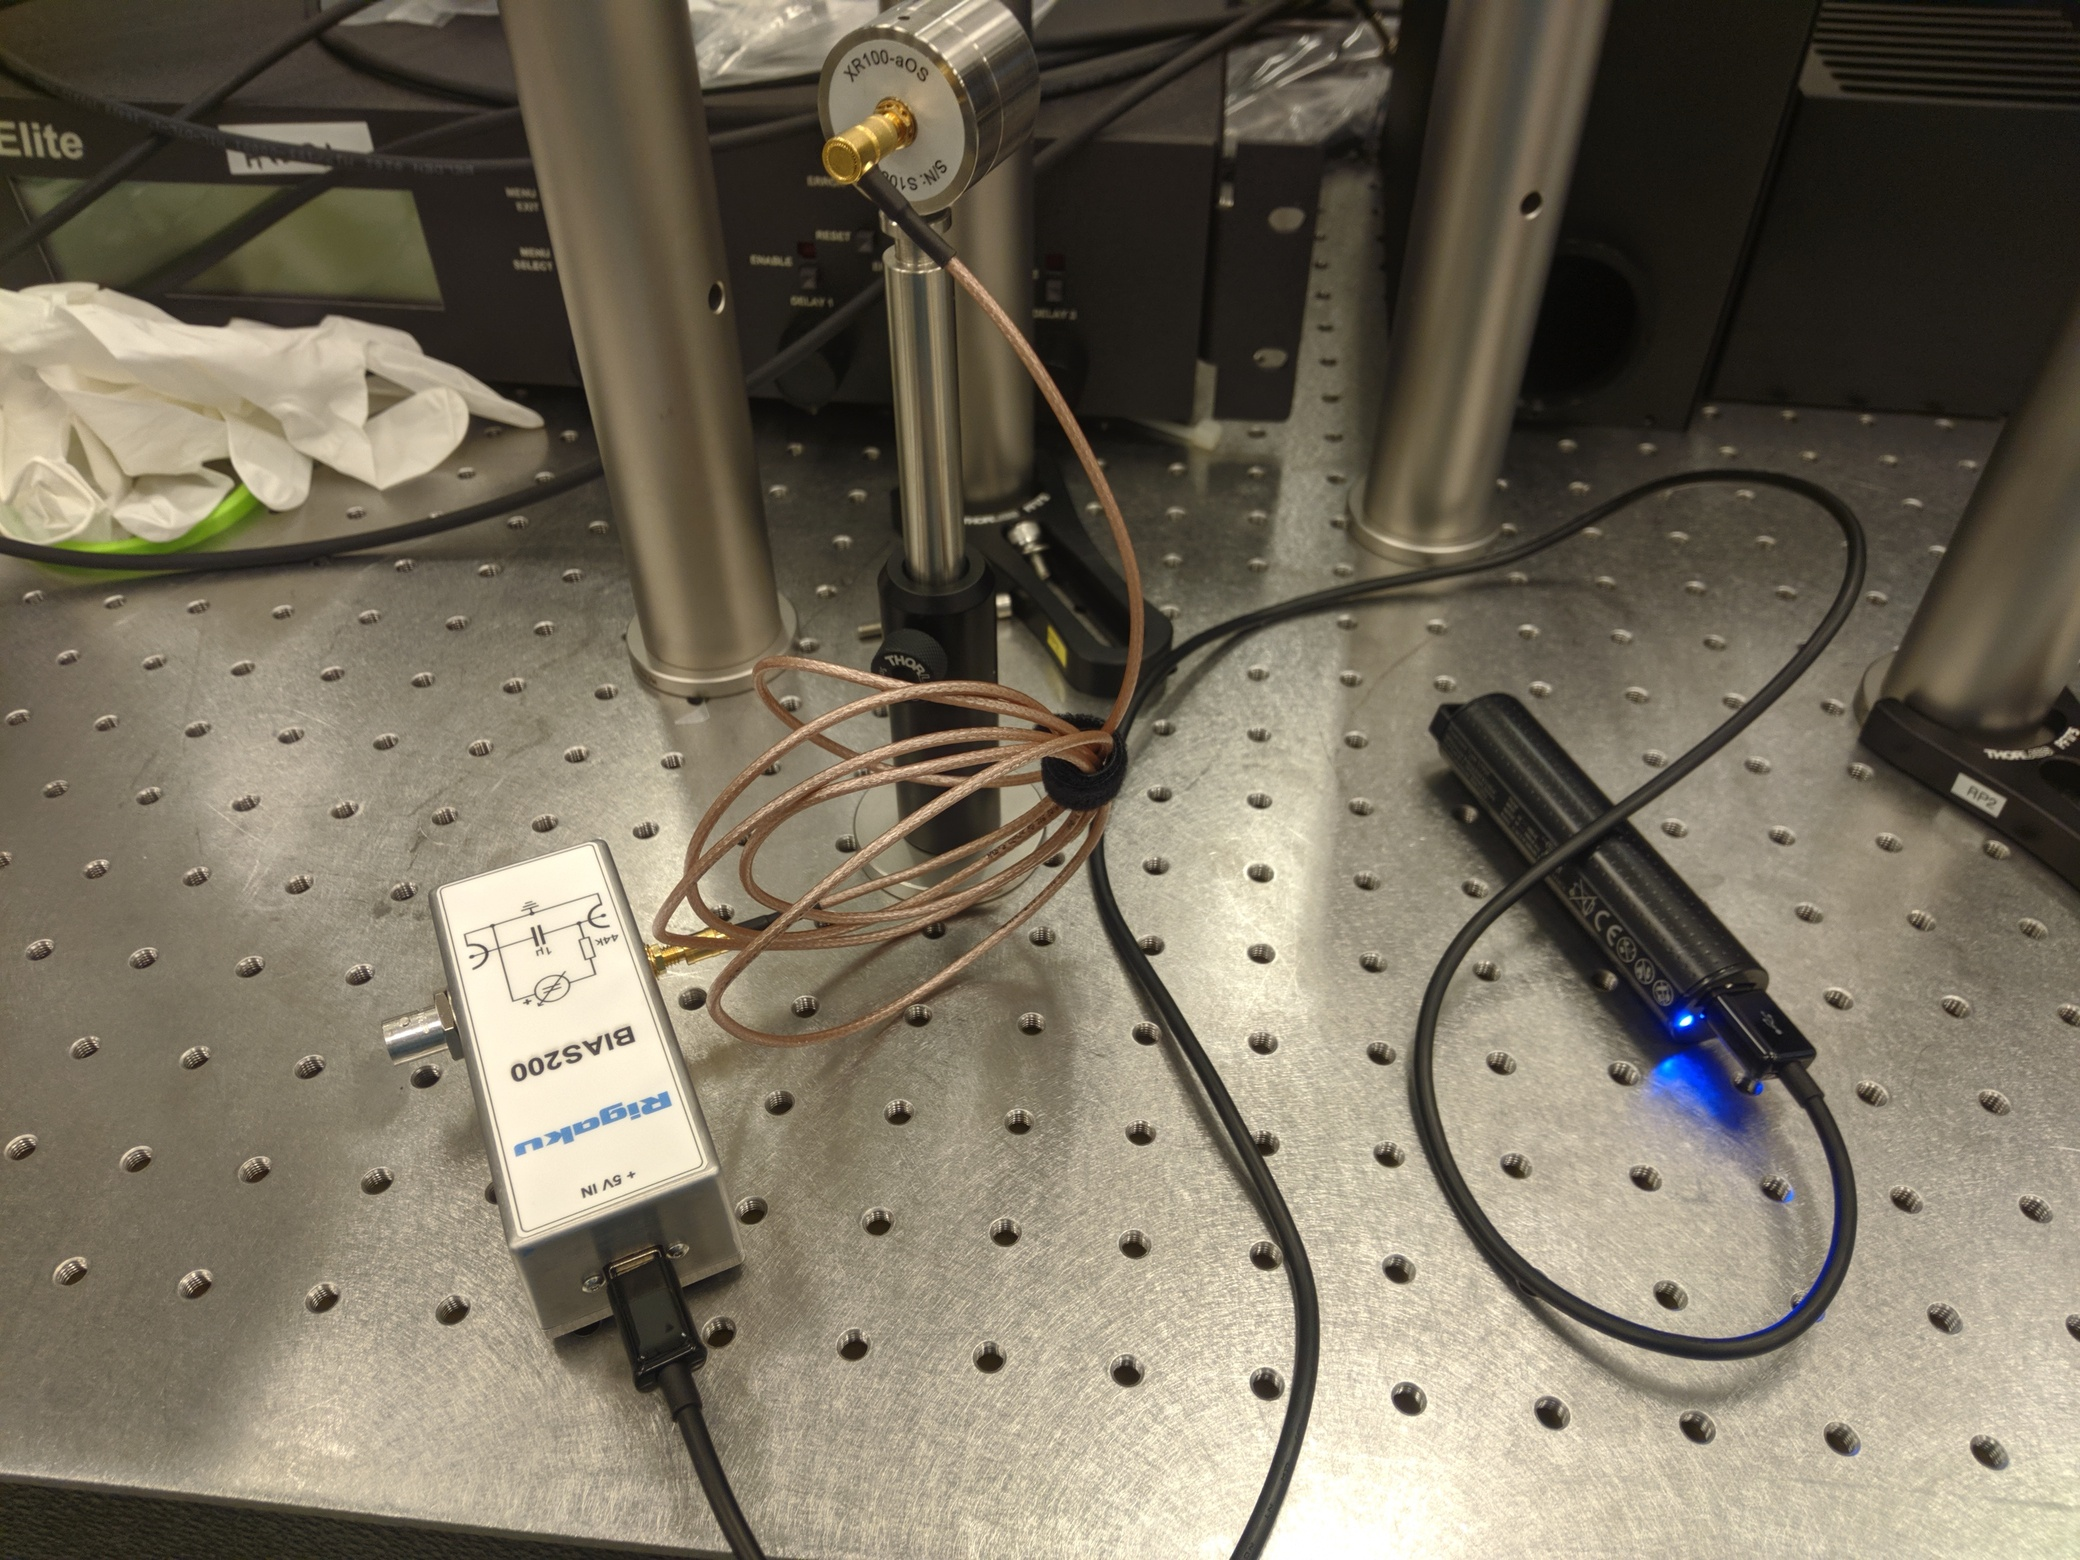
\includegraphics[width=0.8\textwidth]{./images/pin-setup.jpg}
    \caption{The PIN diode setup}
    \label{fig:pin-setup}
\end{figure}

\subsection{Sample and Hold}\label{subsec:sample-hold}
The device referred to when written S\&H is a device built in ELI (shown in \cref{fig:sample-hold}) which contains a Sample and Hold amplifier (its schematics can be seen in \cref{sec:sample-hold-schema}).
The Sample and Hold amplifier is made by DATEL and the product page can be found \href{http://catalog.datel.com/item/data-acquisition-product-line/sample-and-hold-amplifiers/shm-43mc}{here}\footnote{http://catalog.datel.com/item/data-acquisition-product-line/sample-and-hold-amplifiers/shm-43mc}.

The device consists of two parts, the gray box contains the power supply and the green one the Sample and Hold amplifier.
The green box has 4 ports: TRIG IN, TRIG OUT, SIG IN and SIG OUT.
It works as follows: When the voltage on TRIG IN crosses a certain threshold, the device "saves" the value of the voltage on SIG IN and then continues to output that voltage on SIG OUT until the voltage in TRIG IN drops back down.
TRIG OUT just outputs whatever came in on TRIG IN and is not essential for the function.
An image from the S\&H in action is in \cref{fig:sample-hold-osci}.

\begin{figure}[h]
    \centering
    \begin{subfigure}{0.4\textwidth}
        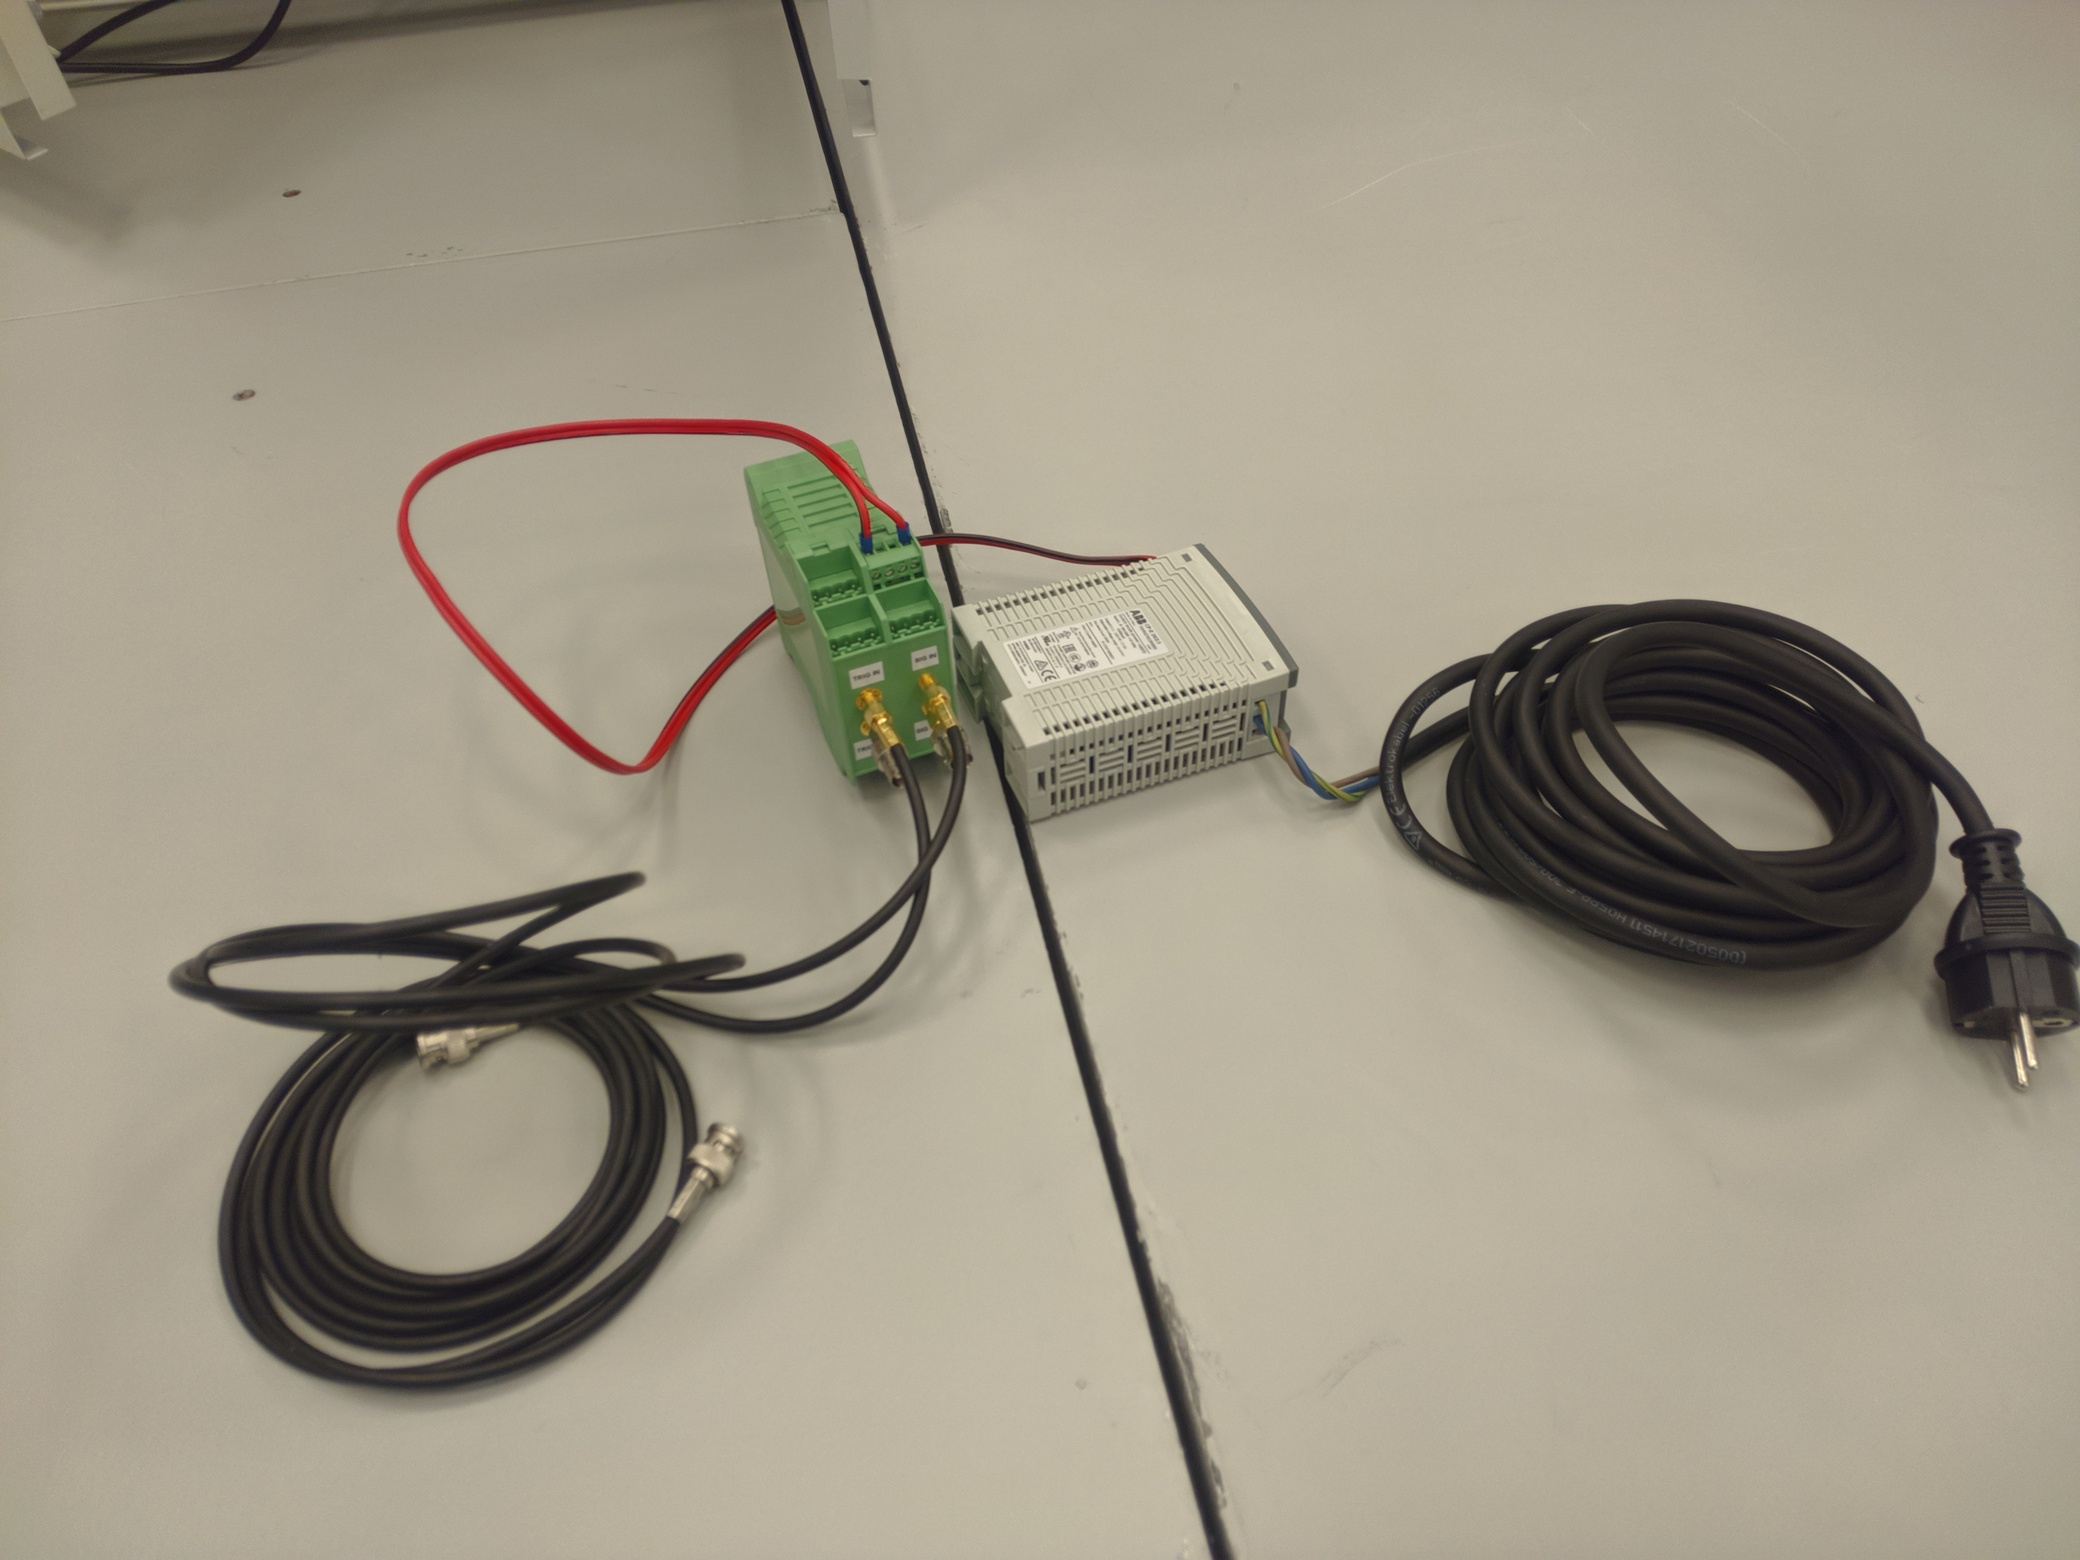
\includegraphics[width=\textwidth]{./images/sample-hold.jpg}
        \caption{Sample and Hold}
        \label{fig:sample-hold-overview}
    \end{subfigure}
    \begin{subfigure}{0.4\textwidth}
        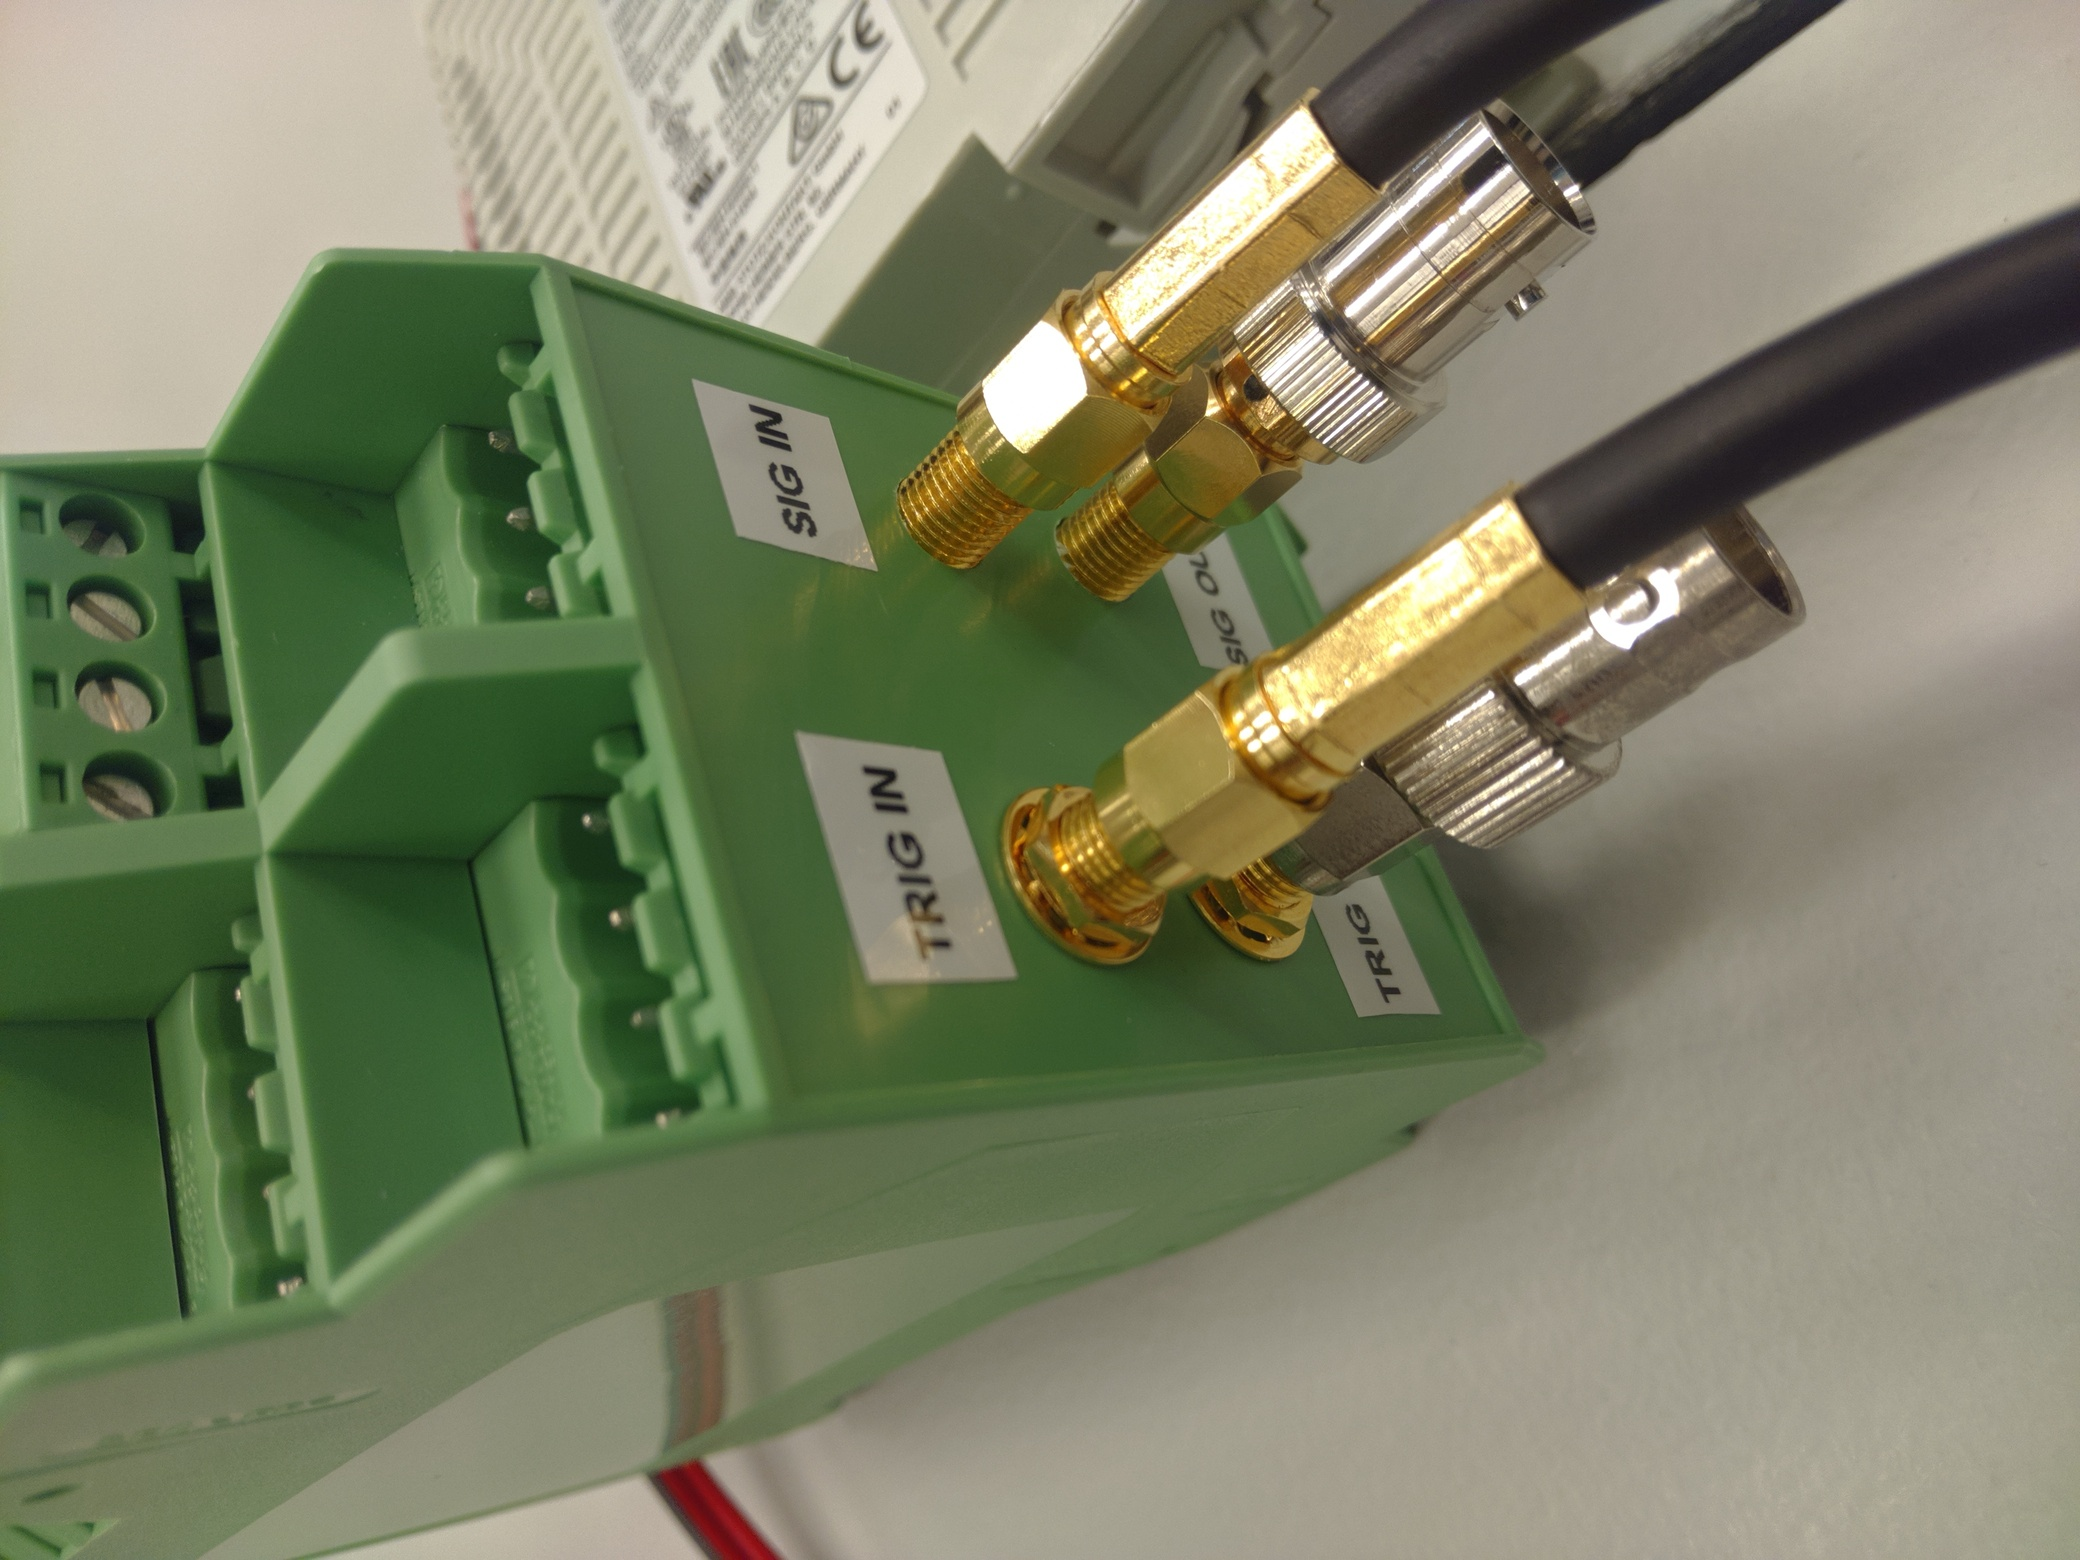
\includegraphics[width=\textwidth]{./images/sample-hold-detail.jpg}
        \caption{Detail of the ports}
        \label{fig:sample-hold-detail}
    \end{subfigure}
    \caption{The Sample and Hold device}
    \label{fig:sample-hold}
\end{figure}

\begin{figure}[H]
    \centering
    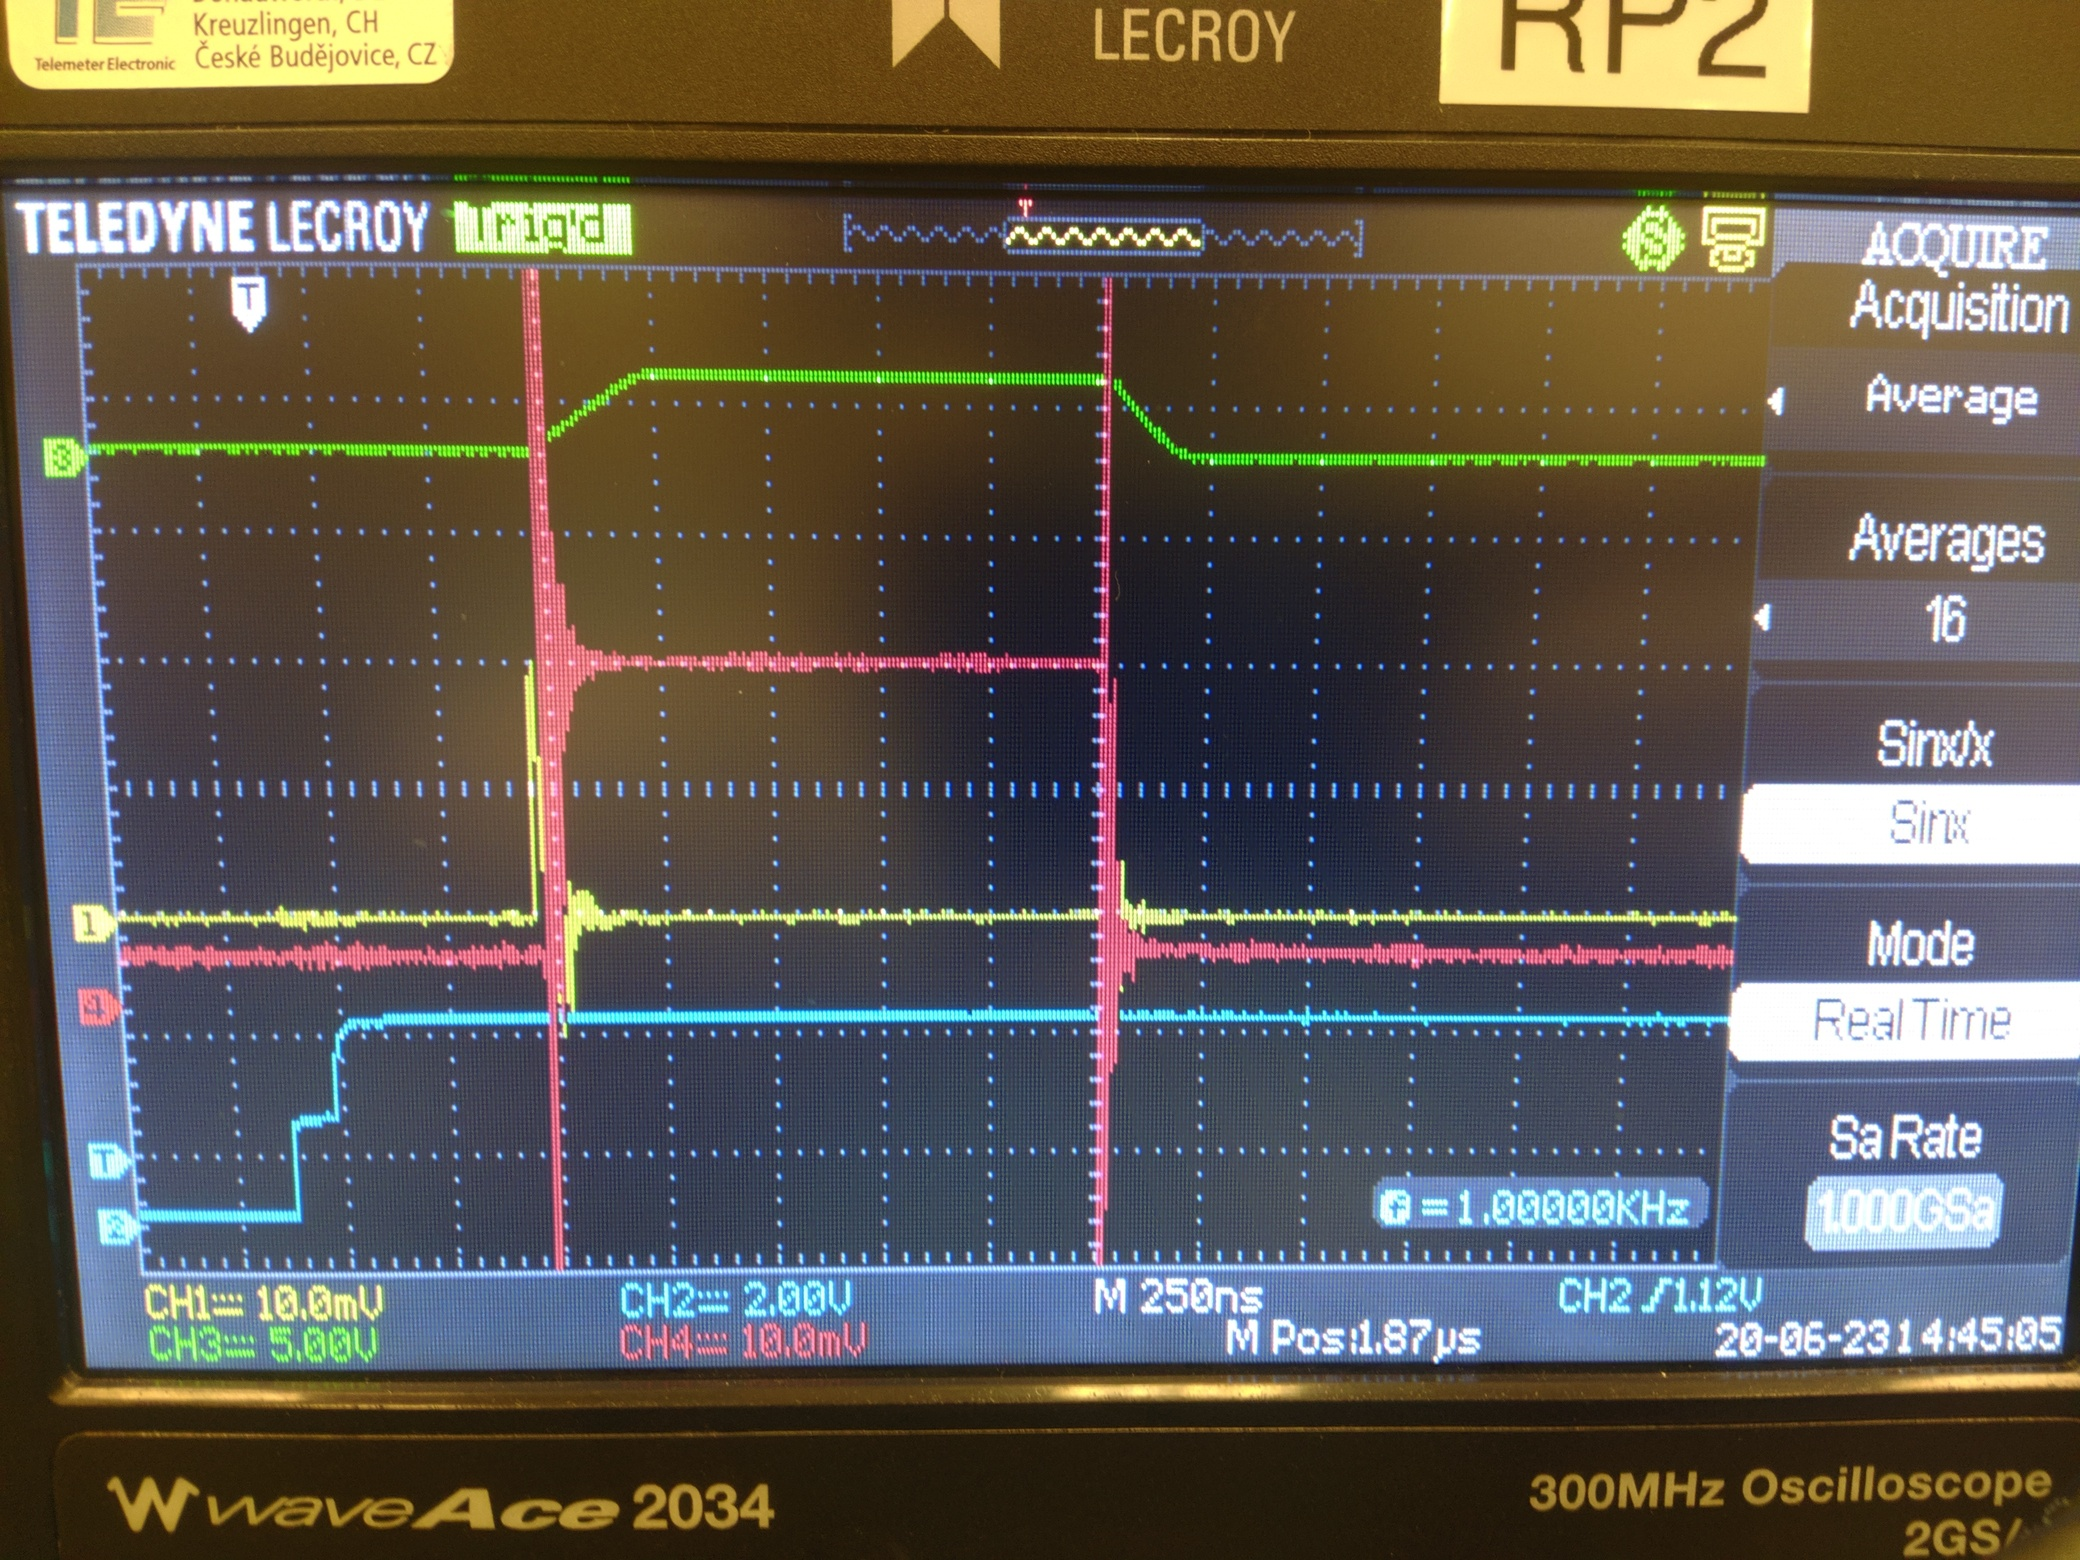
\includegraphics[width=0.8\textwidth]{./images/sample-hold-osci.jpg}
    \caption{Example of the S\&H in action. Green line is TRIG OUT, yellow line is SIG IN, red line is SIG OUT and the blue line is just used as a trigger for the oscilloscope}
    \label{fig:sample-hold-osci}
\end{figure}

There's some more information that needs to be mentioned however.
The first thing is that the S\&H needs the TRIG IN signal to reach at least about 5 \si{\volt} (and it's safe to go up to 9) otherwise it won't trigger.
This is the threshold mentioned before, however it does not actually trigger when TRIG IN reaches the threshold, it triggers when it reaches a smaller value (this is best illustrated in \cref{fig:sample-hold-osci} where you can see the red line triggering when the green line has barely just started going up).

Another thing is that the S\&H changes the input signal.
When tested using a different signal generator instead of the xPIN, the measured voltage was a linear function of the generated function with coefficient a being about 2 and b being -5 \si{\milli\volt}.
During first testing with the xPIN it seemed however that the S\&H just added about 4 \si{\milli\volt}.
The second behavior is shown in \cref{fig:sample-hold-osci-2}.

\begin{figure}[H]
    \centering
    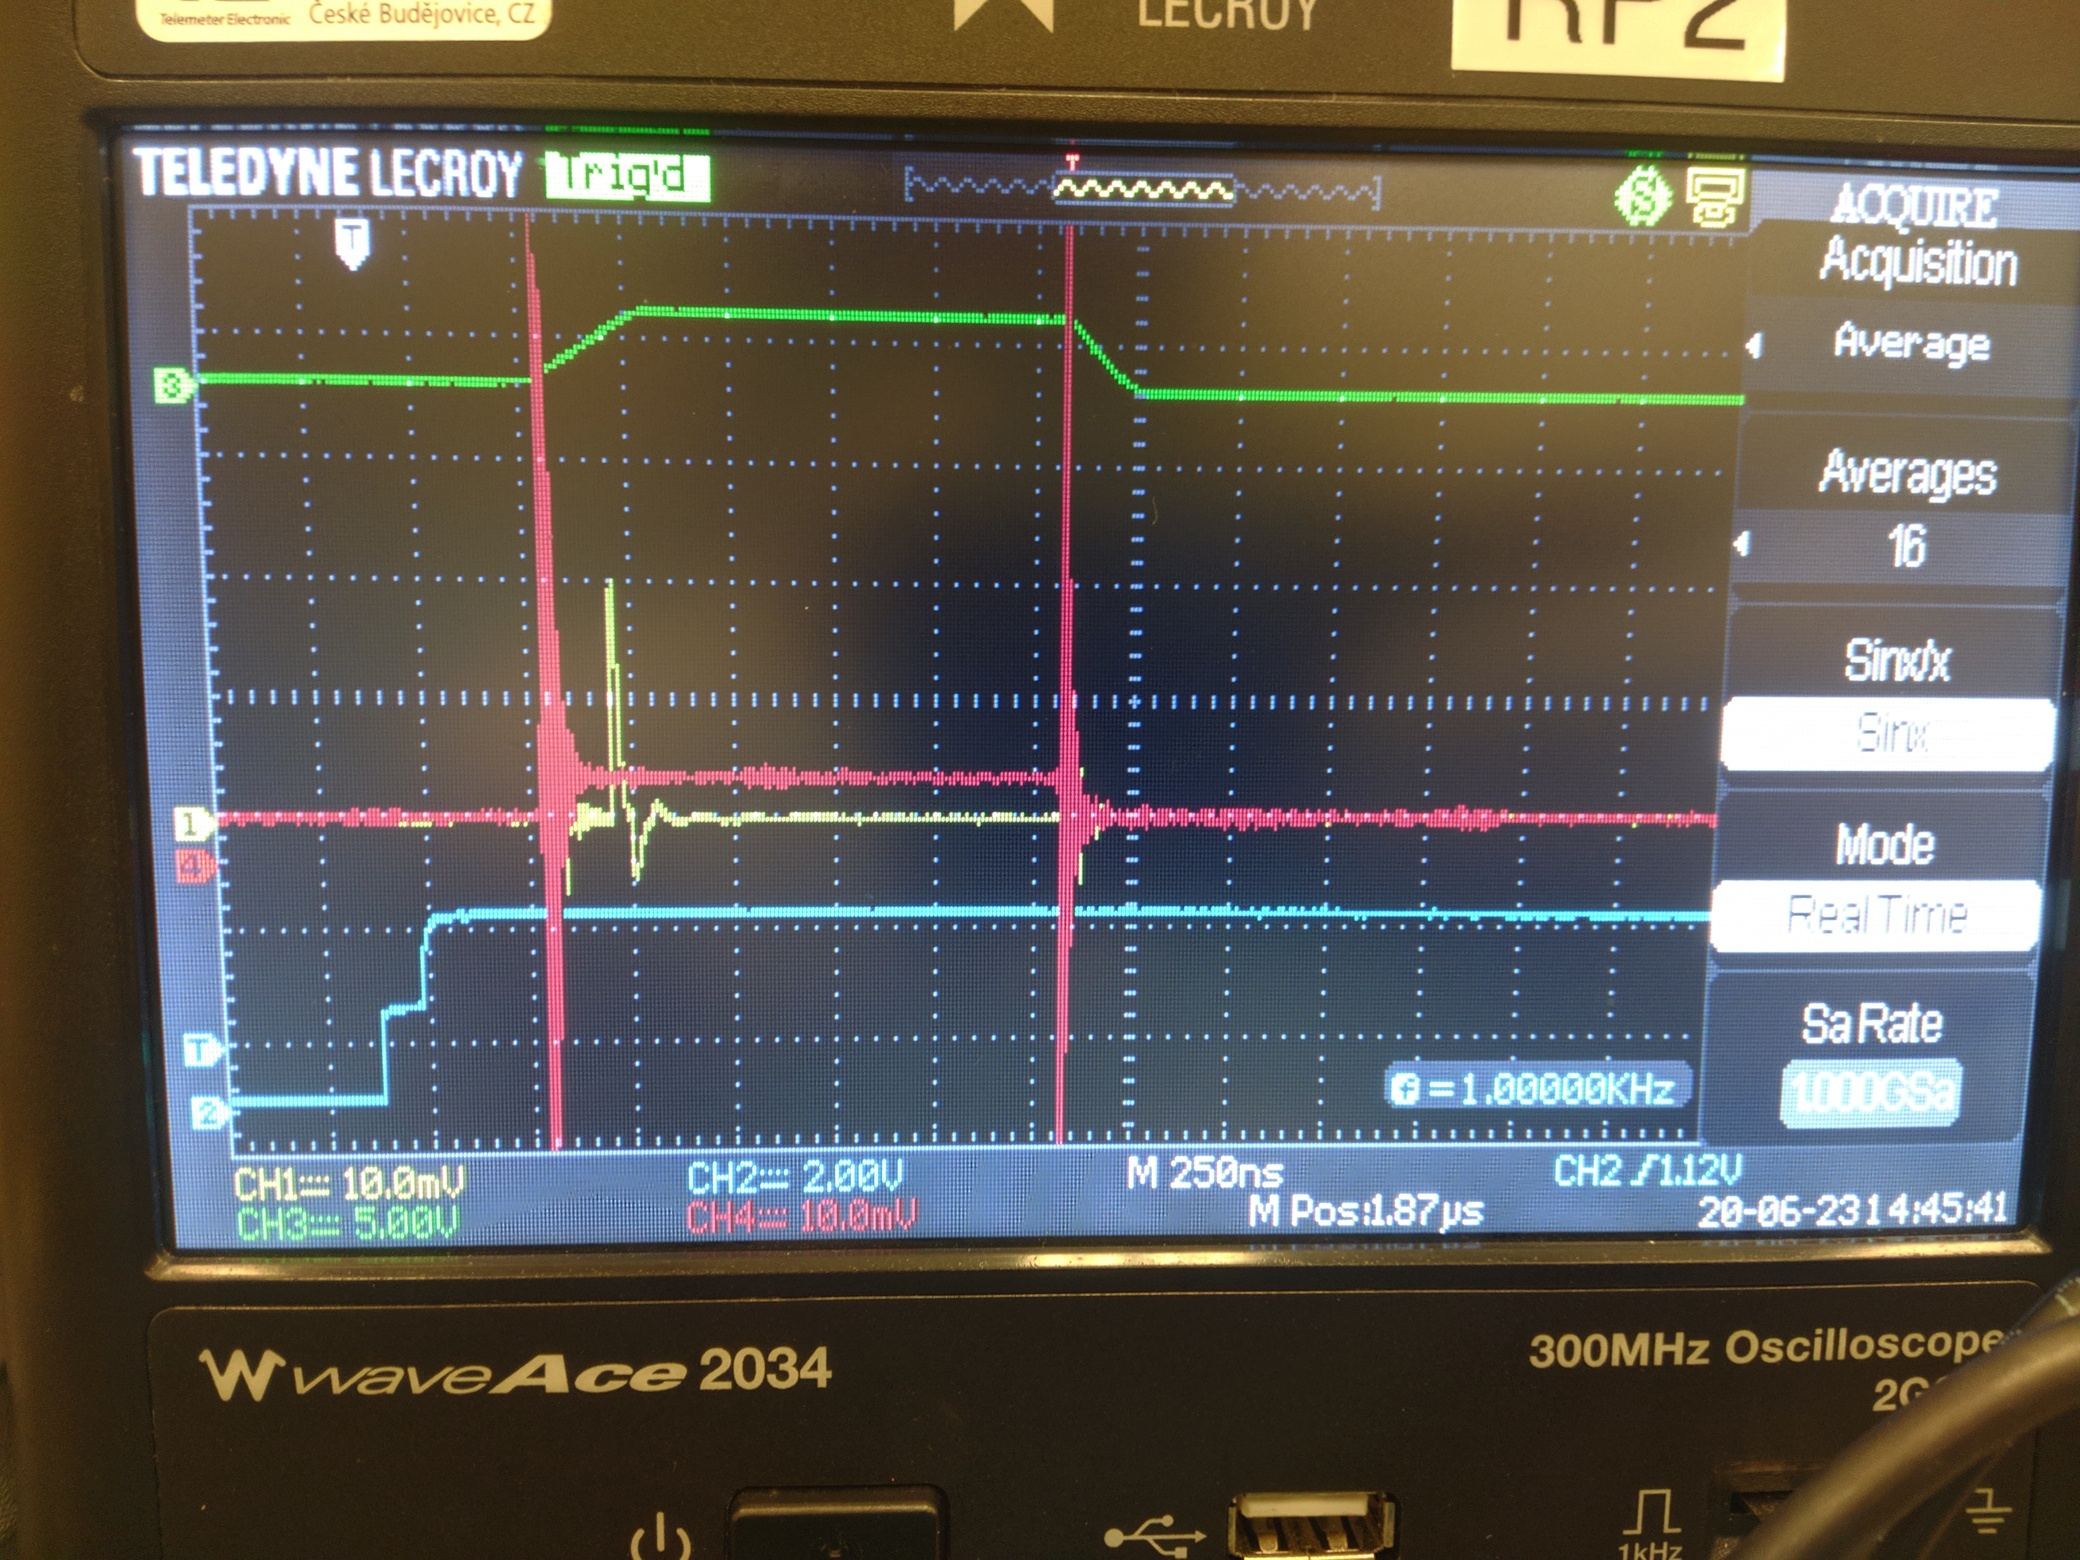
\includegraphics[width=0.9\textwidth]{./images/sample-hold-osci-2.jpg}
    \caption{The connections are the same as in \cref{fig:sample-hold-osci} but this time the S\&H trigger is moved a bit in front of the peak. It is possible to see that the yellow line dips a bit just as the S\&H triggers, this is just an artifact of the S\&H it is not a part of the actual signal. It can also be seen that the red line is about 4 \si{\milli\volt} above the yellow line. This is another artifact of the S\&H.}
    \label{fig:sample-hold-osci-2}
\end{figure}

The S\&H also adds some noise to the signal.
The signal on SIG OUT is more noisy than the one on SIG IN and it is also delayed a bit (about 20 \si{\nano\second}, visible in \cref{fig:sample-hold-osci}).
It also distorts the signal on SIG IN itself, this is visible in \cref{fig:sample-hold-dist}.

\begin{figure}[H]
    \centering
    \begin{subfigure}{0.5\textwidth}
        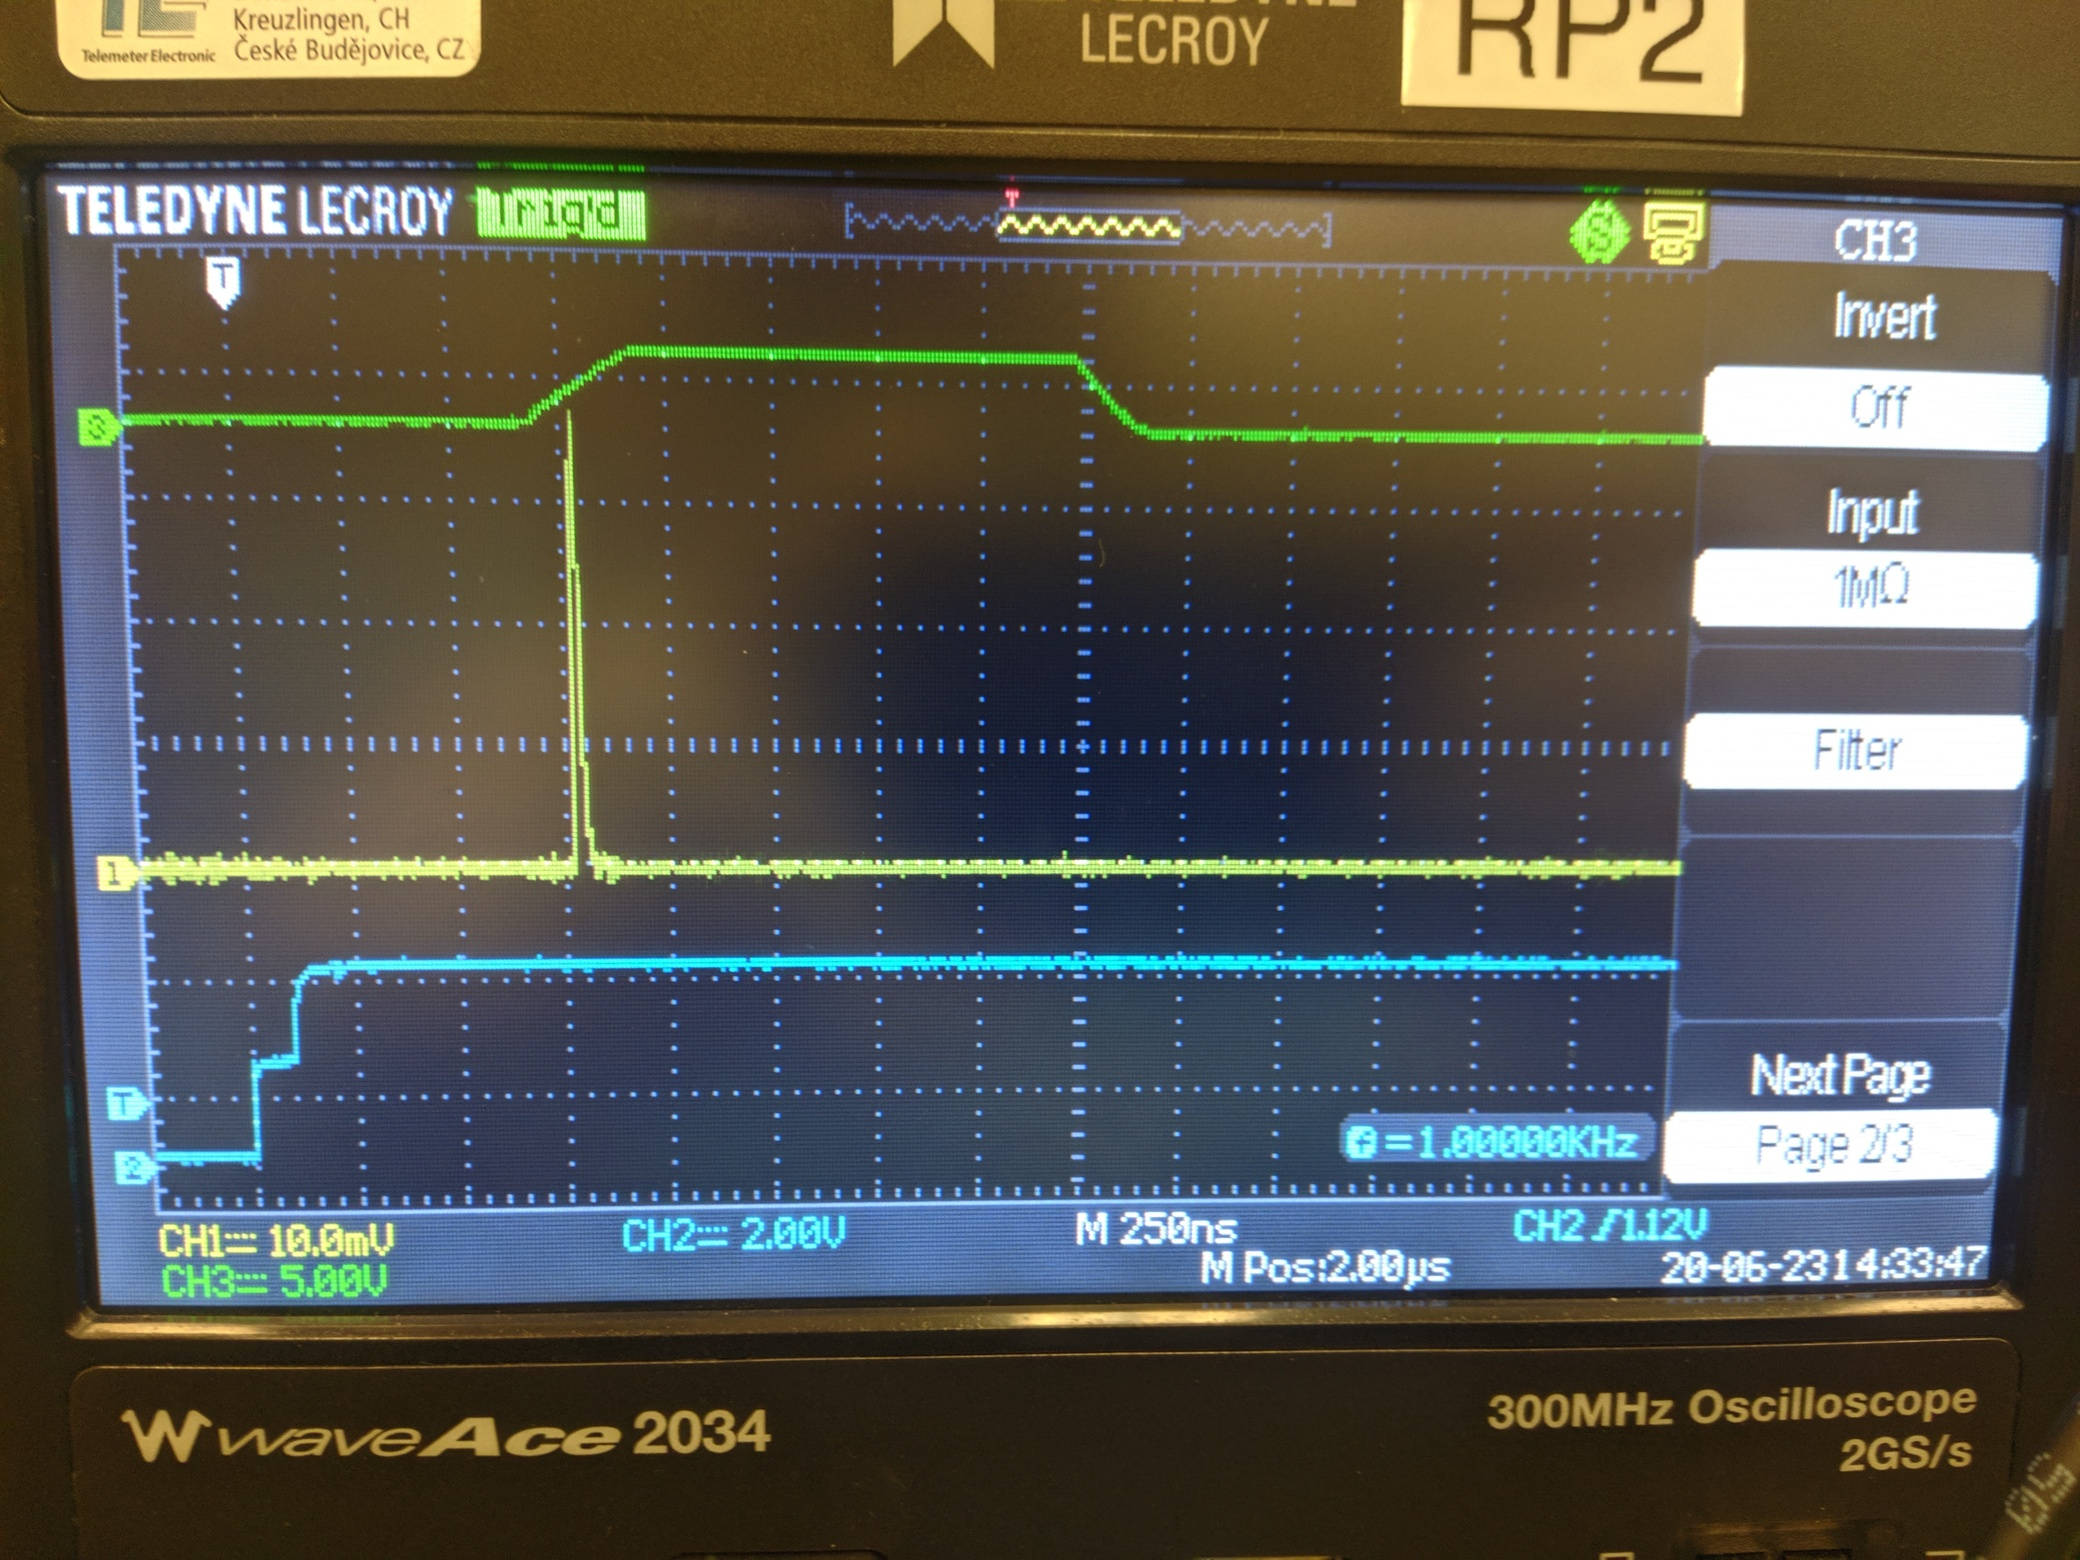
\includegraphics[width=\textwidth]{./images/sample-hold-pin-clean.jpg}
        \caption{PIN diode output when the S\&H is disconnected.}
        \label{fig:sample-hold-pin-clean}
    \end{subfigure}
    \begin{subfigure}{0.5\textwidth}
        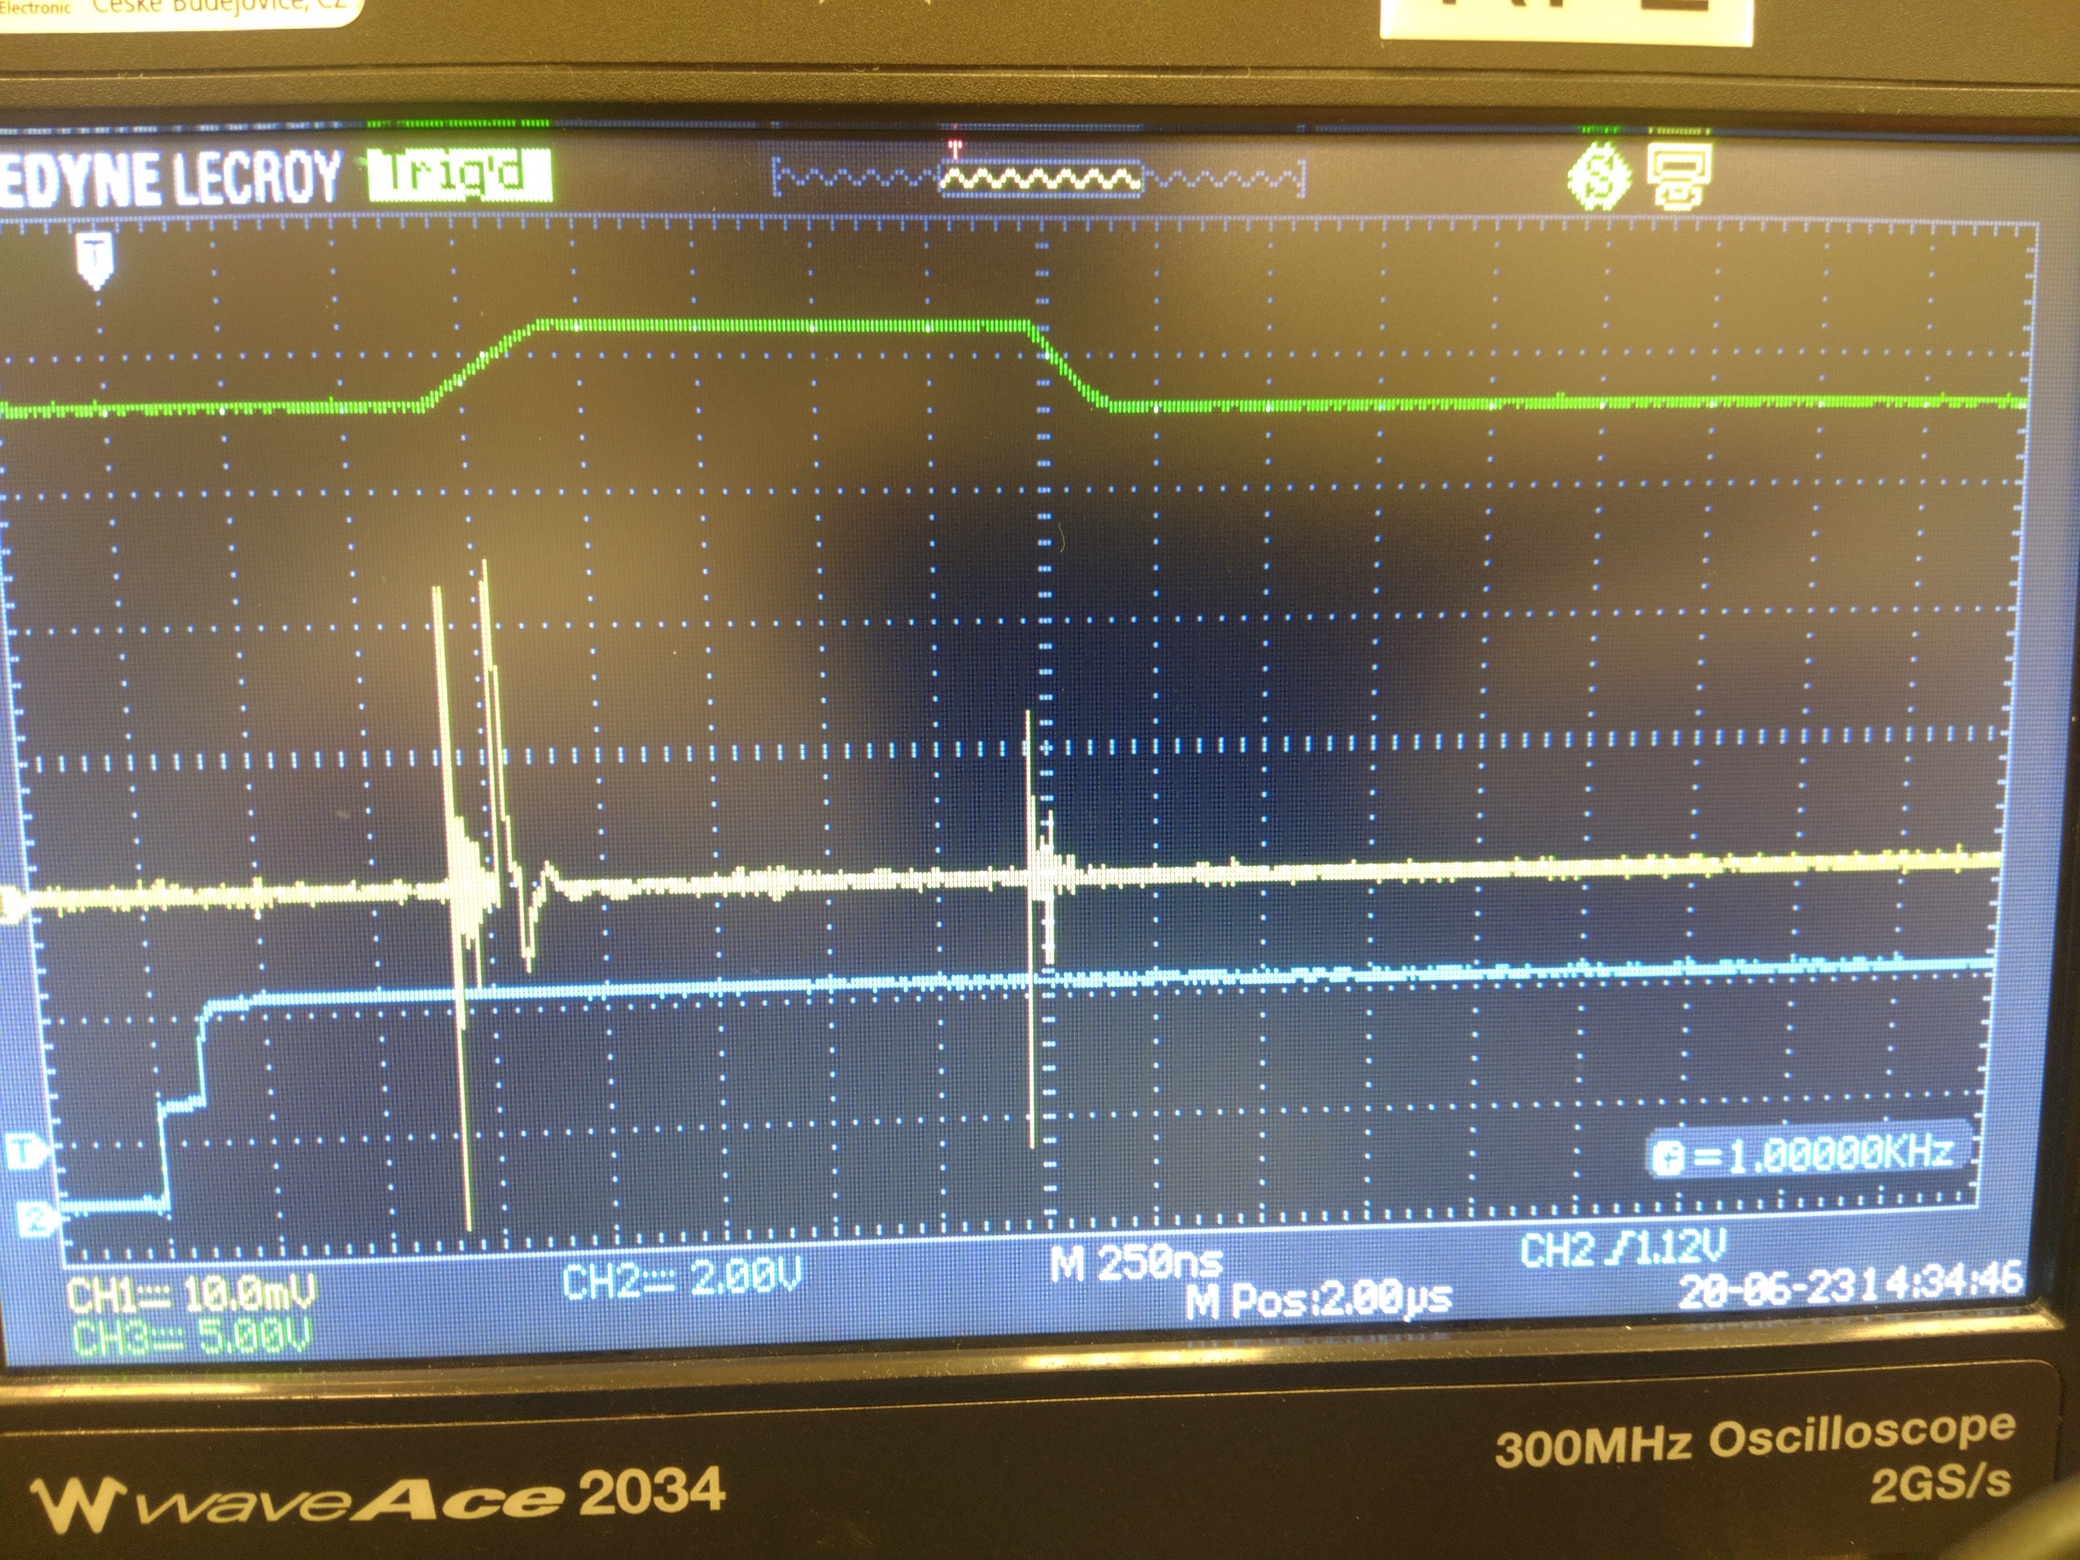
\includegraphics[width=\textwidth]{./images/sample-hold-pin-dist.jpg}
        \caption{PIN diode output when the S\&H is connected.}
        \label{fig:sample-hold-pin-dist}
    \end{subfigure}
    \caption{This figure shows how the S\&H distorts its input signal. The connections are again the same as in \cref{fig:sample-hold-osci}.}
    \label{fig:sample-hold-dist}
\end{figure}

Finally while the S\&H hold the signal, the voltage it outputs slowly decays.
It can be seen in figure \cref{fig:sample-hold-decay} where it decays by about 4 \si{\milli\volt} in just under 500 \si{\micro\second}.

\begin{figure}[H]
    \centering
    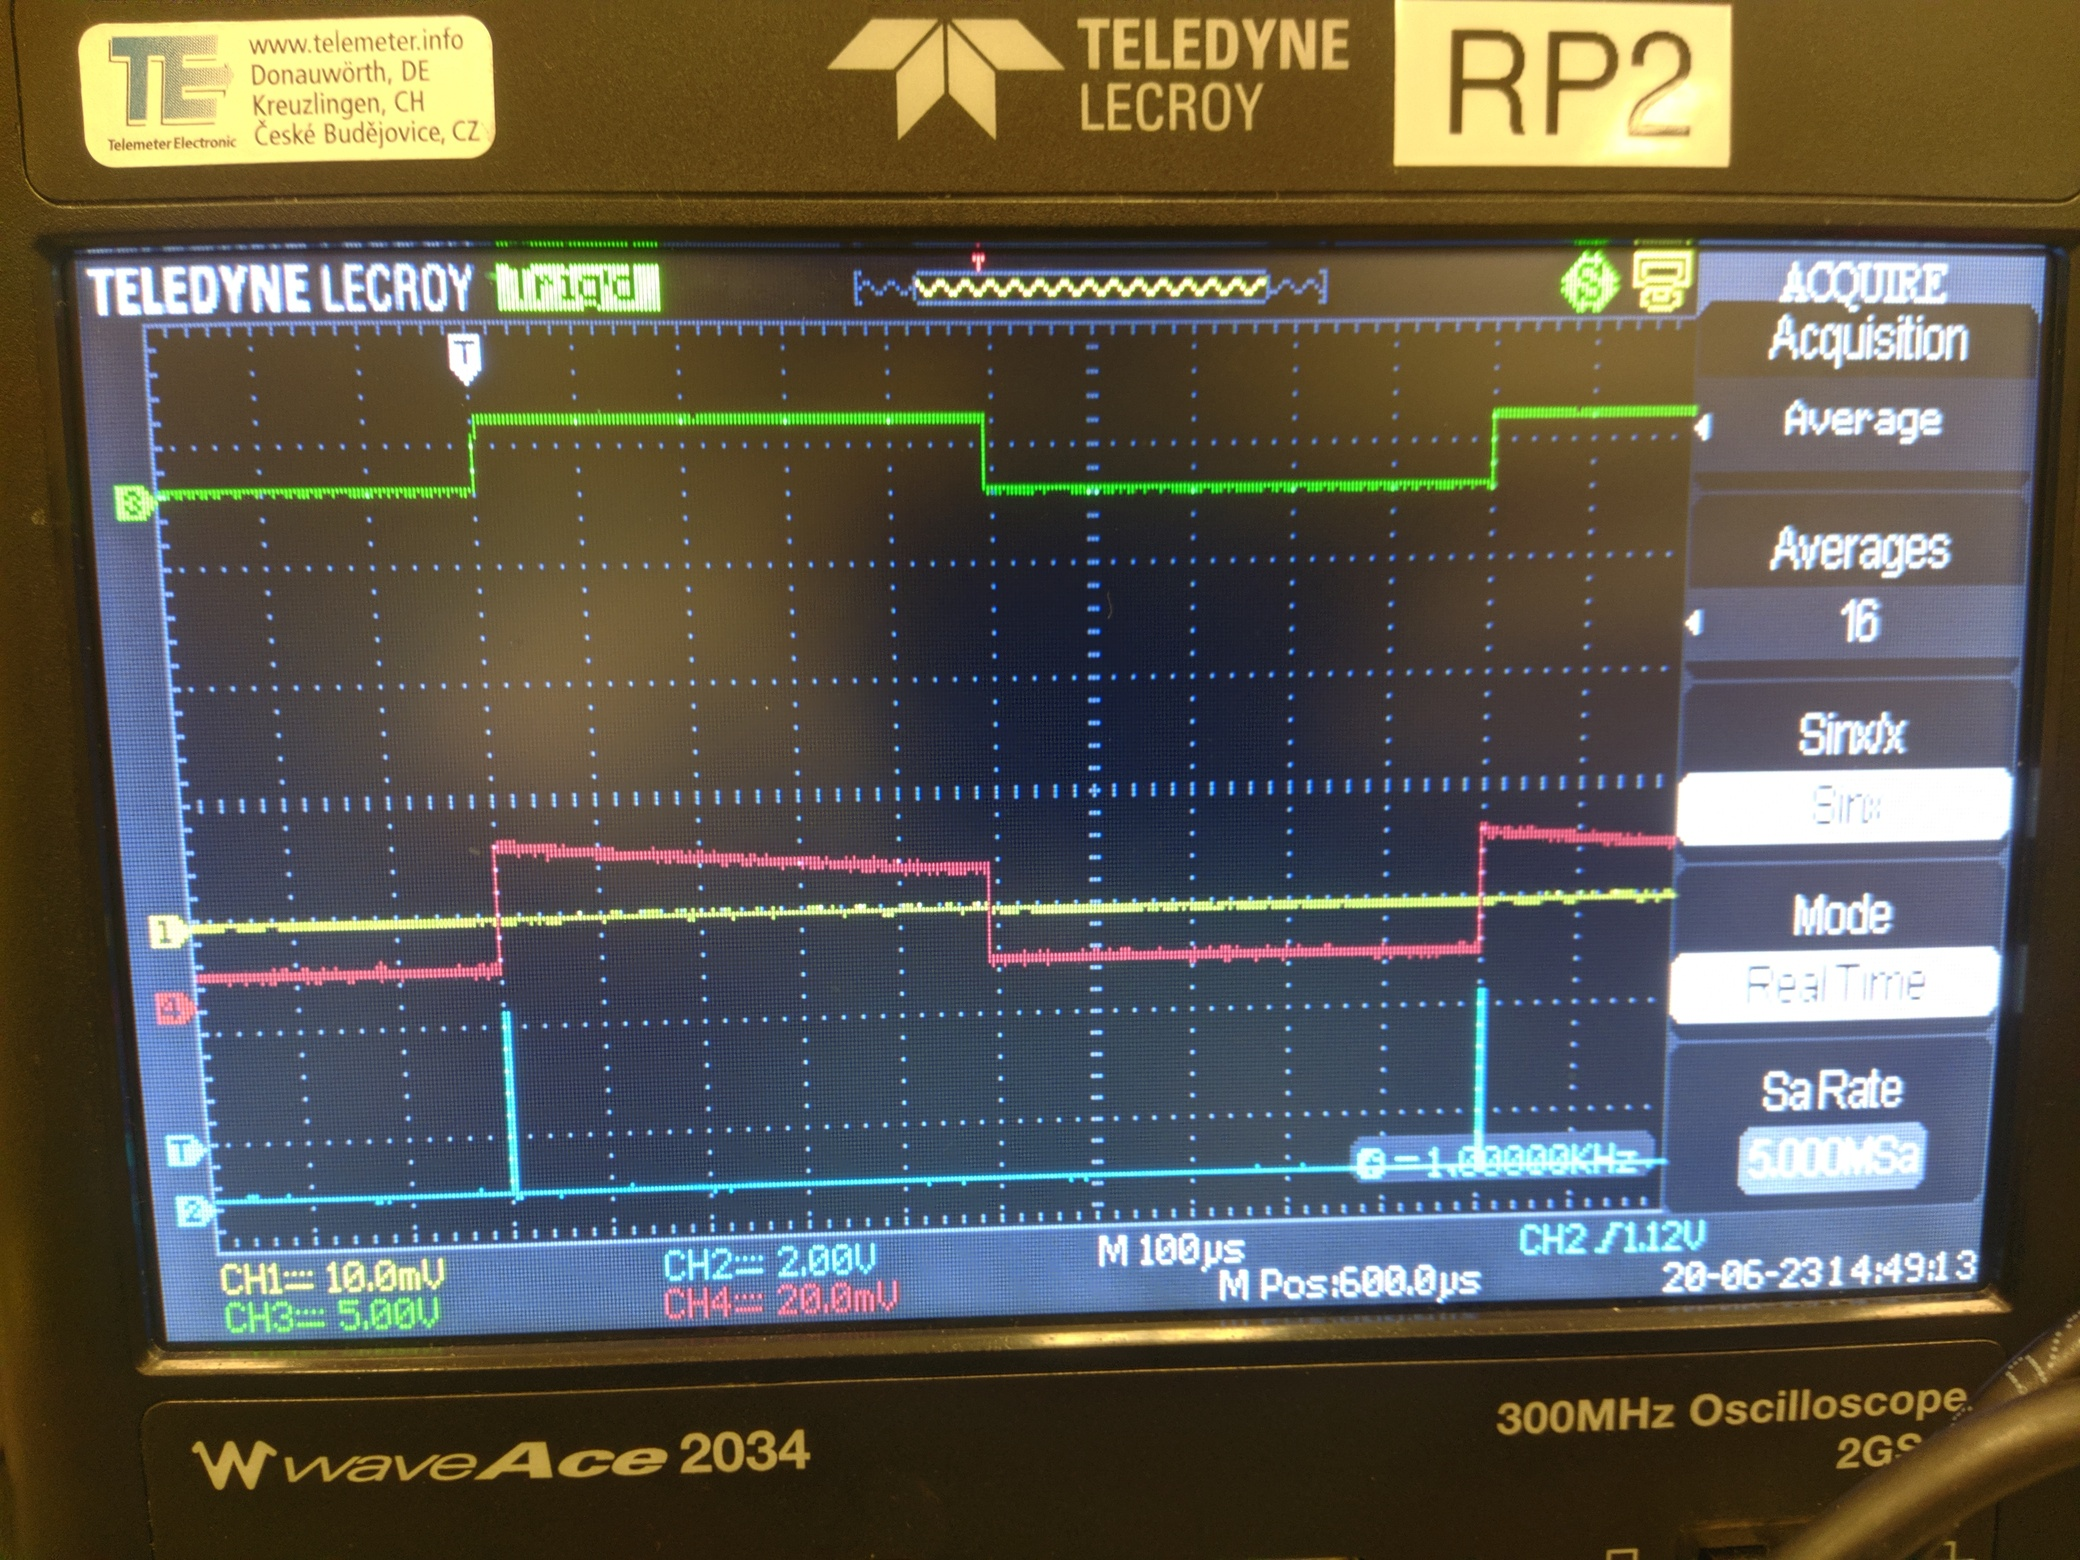
\includegraphics[width=0.5\textwidth]{./images/sample-hold-decay.jpg}
    \caption{The mentioned decay of the SIG OUT voltage during the trigger. Connections are the same as in \cref{fig:sample-hold-osci}.}
    \label{fig:sample-hold-decay}
\end{figure}

\subsection{NI-6002} \label{subsec:sample-hold}
This is a data acquisition device made by National Instruments, the product page can be found \href{https://www.ni.com/cs-cz/support/model.usb-6002.html}{here}\footnote{https://www.ni.com/cs-cz/support/model.usb-6002.html}.
This device can do a variety of things but the only thing we need it for is the analog input port (it can capture at frequencies up to 50 \si{\kilo\hertz}).
We are using it in the single-ended mode, more specifically we have the S\&H output connected to the AI0 and AI GND ports (AI0 is important as otherwise the software won't work with it).
Along with this you will need a computer with the custom software installed on it.

\subsection{Notes on other equipment}
To use the S\&H it is necessary to get a trigger signal that is synchronised with the photon pulses and both it's delay and width are adjustable.
For that we use a signal generator in the "triggered" and "pulse delay" modes.
The one we use can be seen in \cref{fig:signal-generator}

\begin{figure}[H]
    \centering
    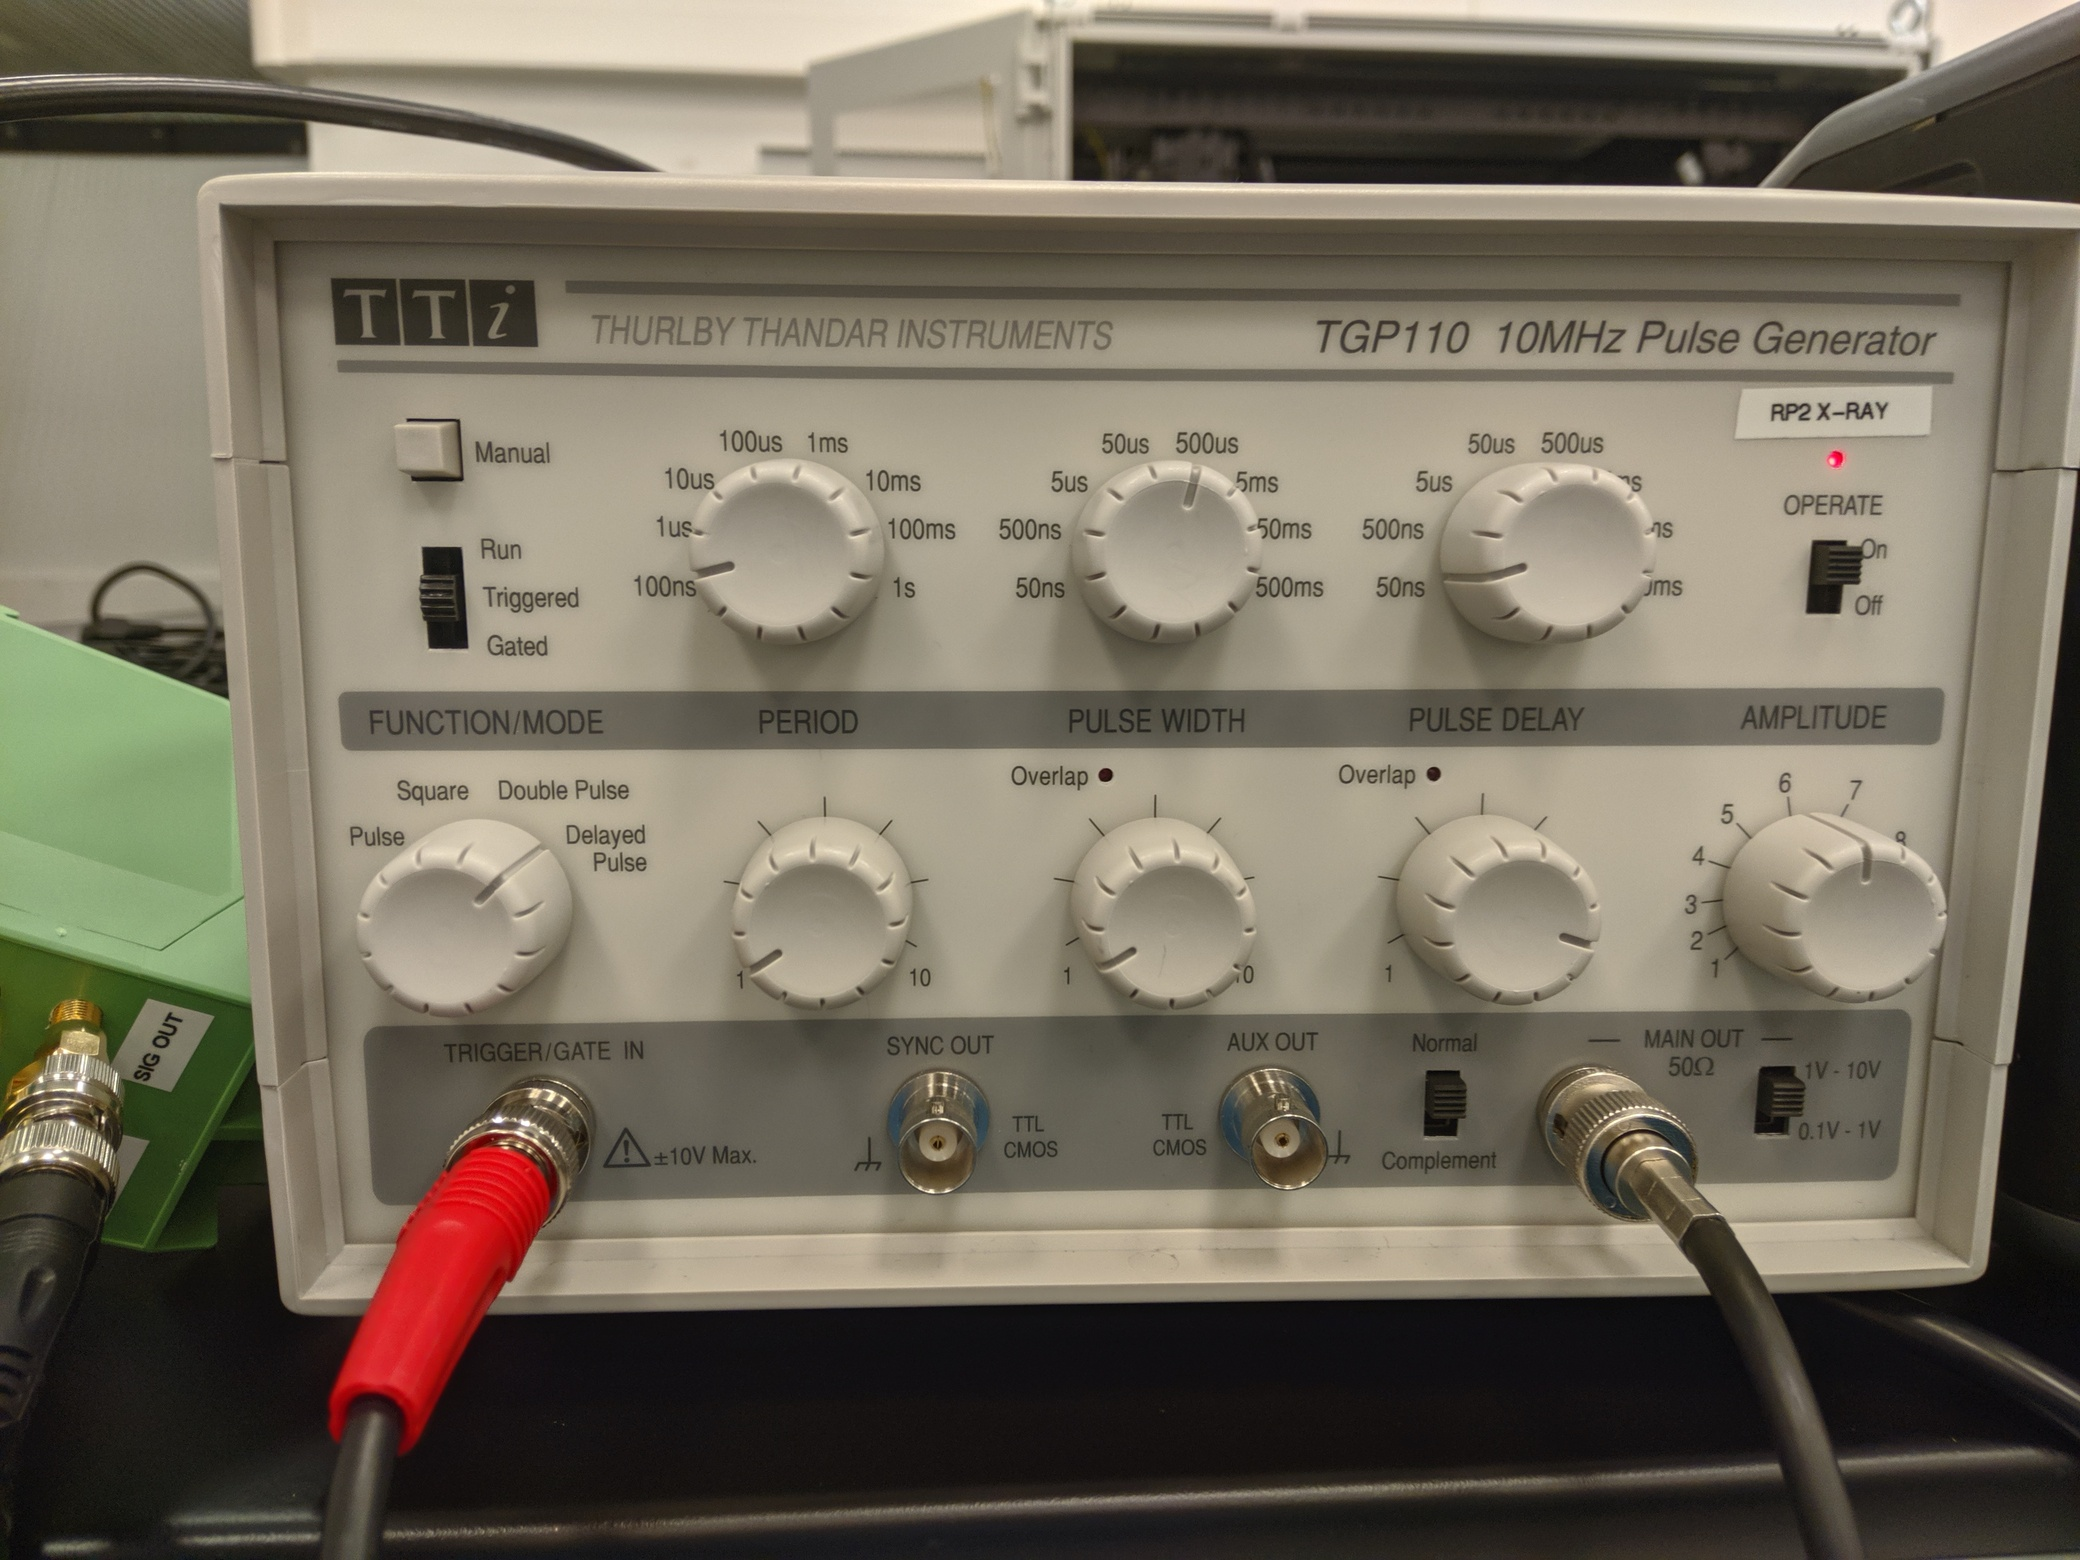
\includegraphics[width=0.9\textwidth]{./images/signal-generator.jpg}
    \caption{The signal generator we use as the S\&H trigger.}
    \label{fig:signal-generator}
\end{figure}

The S\&H is also mainly useful to capture the data, however that part is currently not described in the manual so there will be parts necessary for that.

\section{Connecting it together}
After you secure the photon source and the trigger signal, set up the diode and check it's output using an oscilloscope (using the trigger signal as a trigger for the oscilloscope).
Once you get stable data there you can start setting up the S\&H.

First get the signal generator (SG) and set it in "triggered" mode, use the photon trigger signal as the SG trigger.
Also set the SG to "pulse delay" or equivalent mode, set the delay to 0 and the pulse width to something reasonable.
Once again you may check on the oscilloscope if it works as expected.
Then connect the SG output to TRIG IN on the S\&H and if your oscilloscope has enough ports you may also connect the TRIG OUT to it (which will help get the delay right).
Then connect the PIN output to SIG IN on the S\&H and once again you may use a BNC splitter to also get the raw PIN output.
The last step is to connect the SIG OUT to the oscilloscope.

Then you need to make some adjustments.
Firstly, in \cref{subsec:sample-hold} it was mentioned how the S\&H adds a fixed amount of voltage during the trigger.
If you are observing the data directly on the oscilloscope you may want to adjust for that now.
Just move the delay somewhere where the input is on its zero and then adjust the line height of the SIG OUT line (on the oscilloscope) so that the line during the trigger is at some baseline.
Later you can get the voltage with respect to this baseline which will give you the correct data.
After this step the oscilloscope should look like in \cref{fig:config-height-adjust}.

\begin{figure}[H]
    \centering
    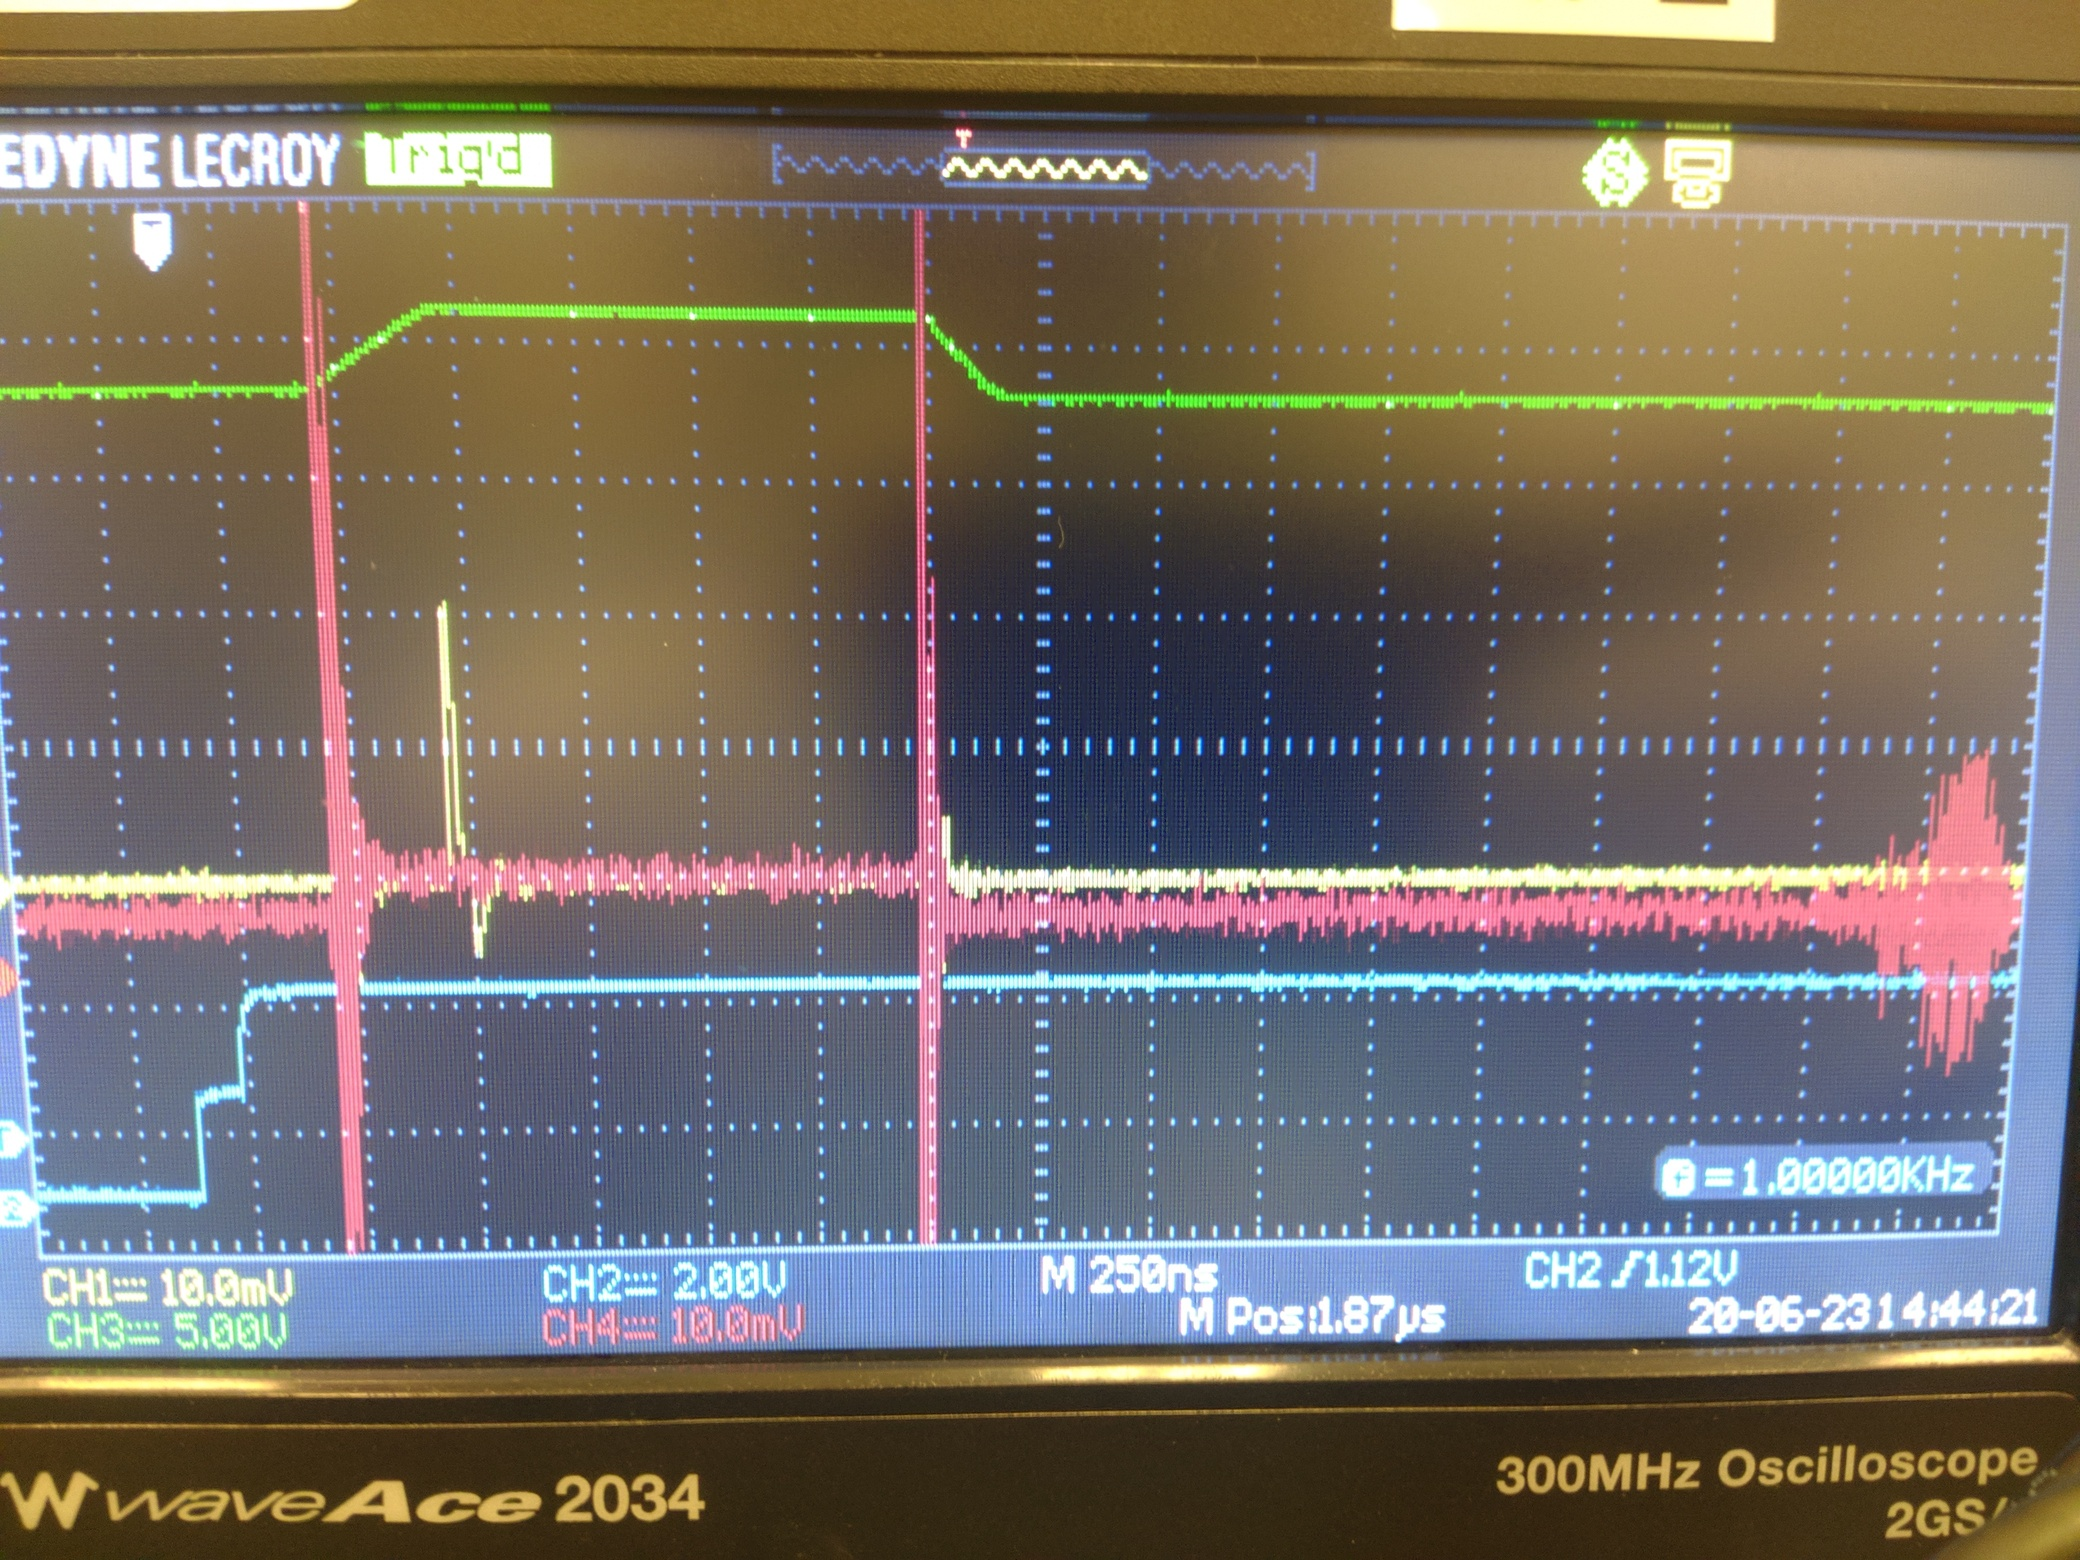
\includegraphics[width=0.9\textwidth]{./images/config-height-adjust.jpg}
    \caption{This shows how the oscilloscope should look after adjusting the SIG OUT line height. Once again connections are the same as in \cref{fig:sample-hold-osci}.}
    \label{fig:config-height-adjust}
\end{figure}

Now you need to adjust the trigger delay.
Simply move the pulse delay so that the S\&H trigger aligns with the PIN output peak.
Keep in mind that the S\&H delays the pulse slightly so you will need the trigger to happen slightly after the peak.
Once it has been set correctly the voltage during the trigger should rise to be the same as the voltage of the peak on the PIN.

\begin{figure}[H]
    \centering
    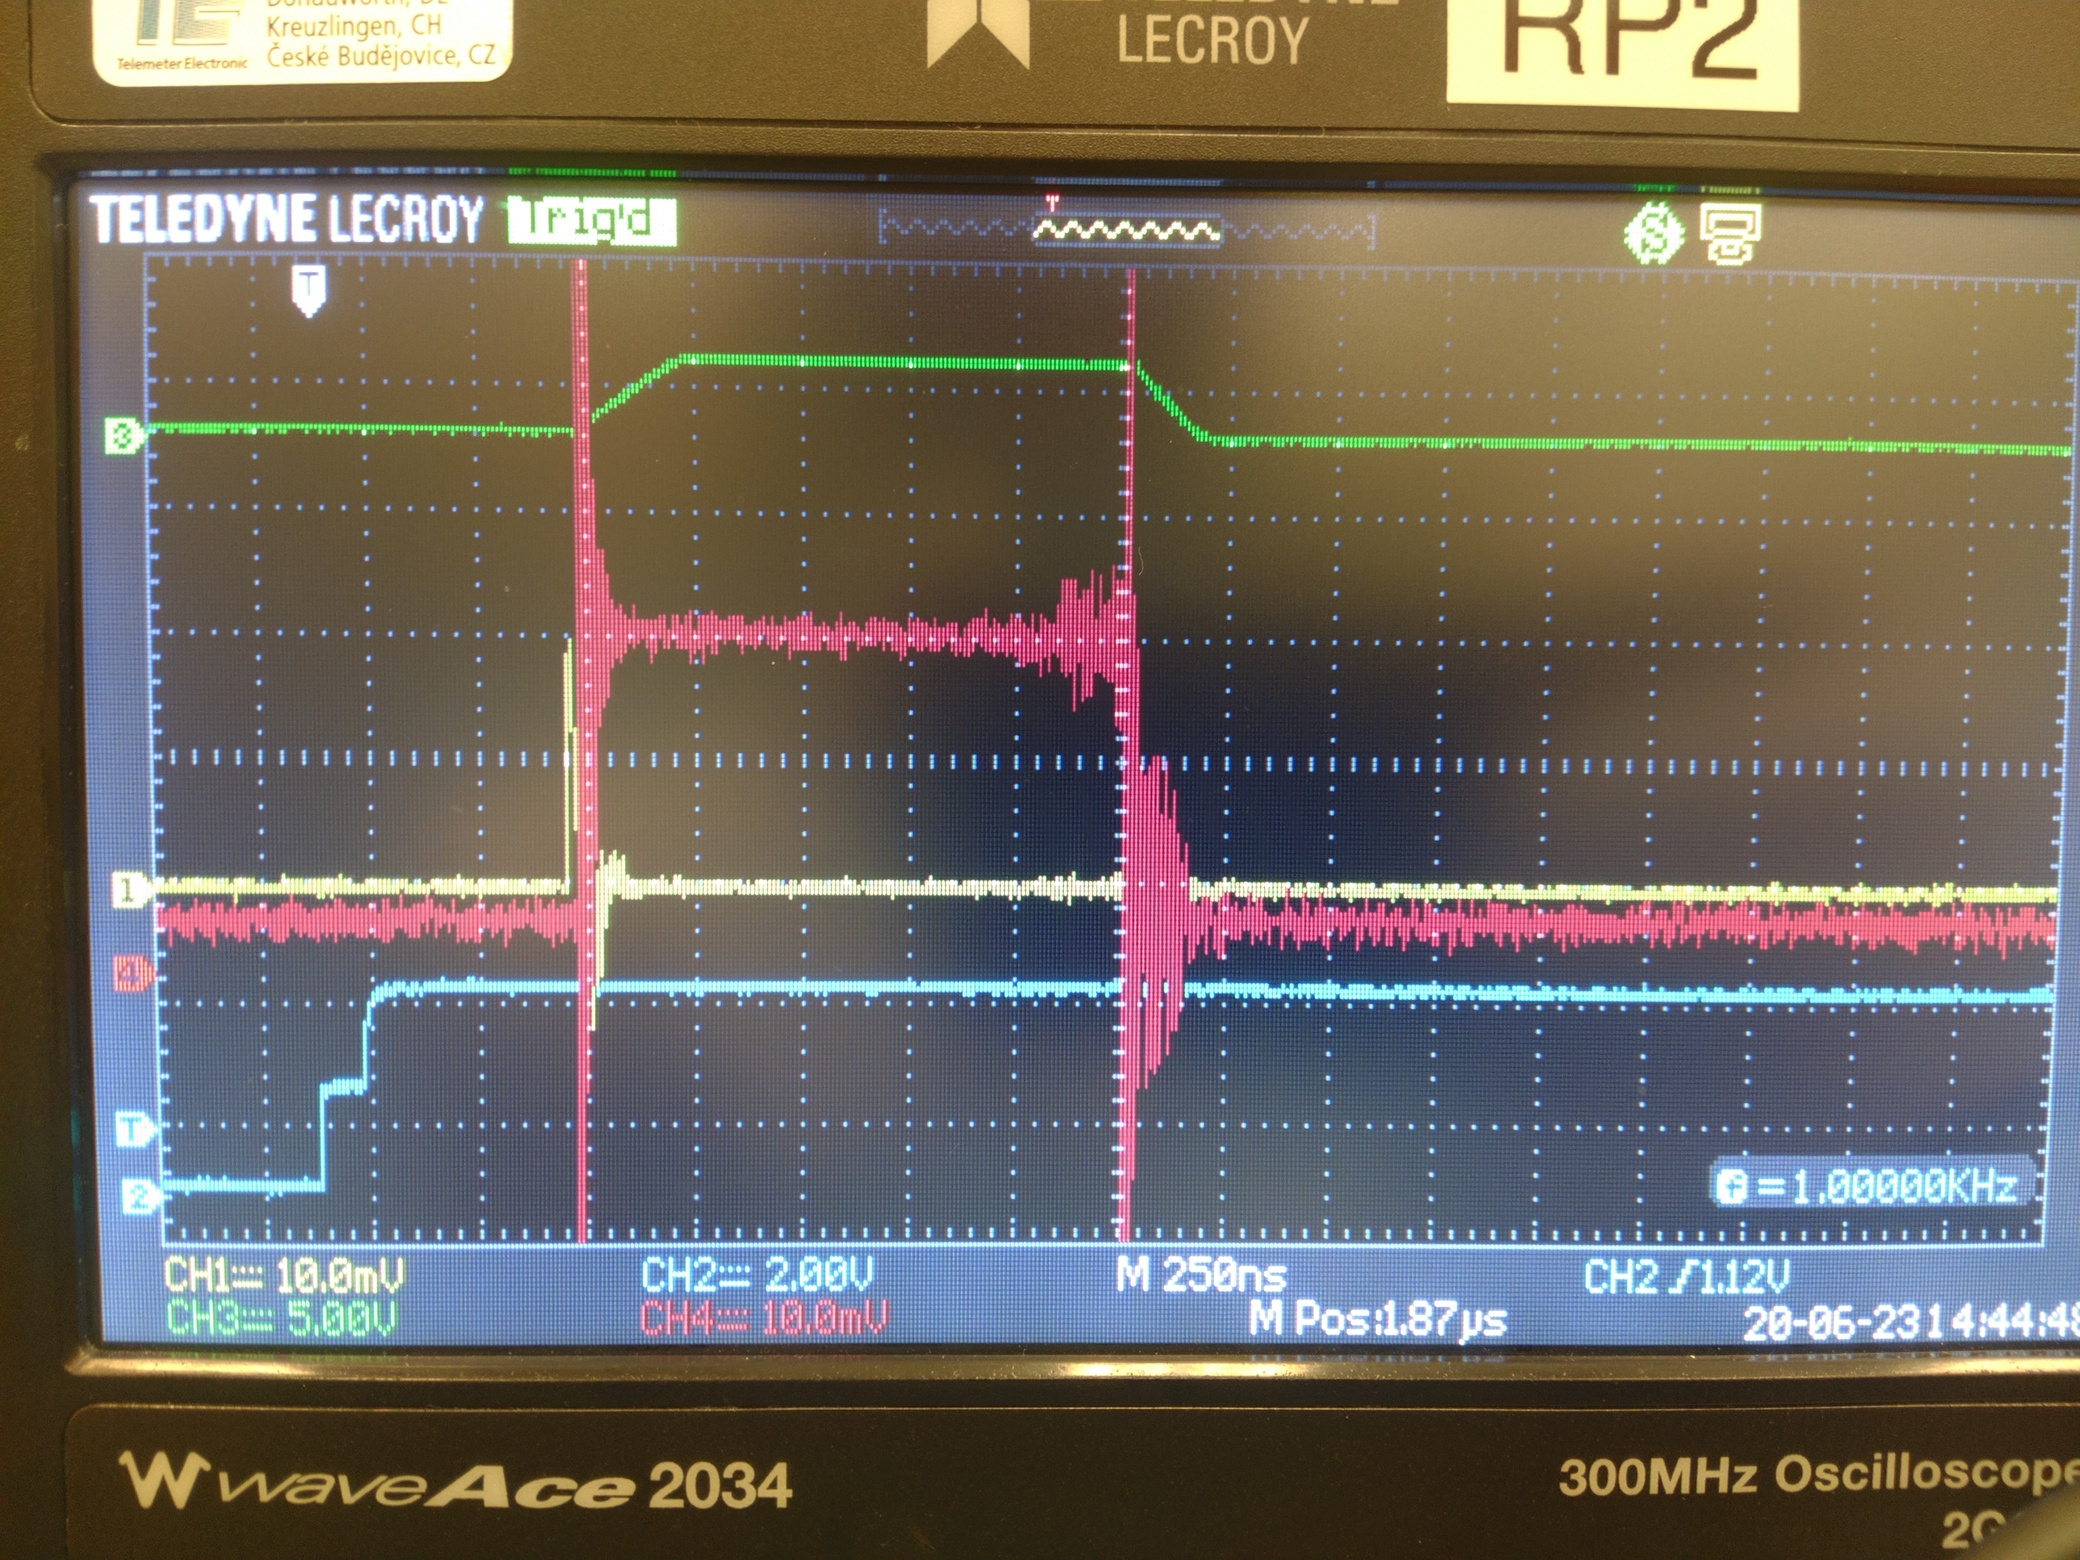
\includegraphics[width=0.9\textwidth]{./images/config-delay-aligned.jpg}
    \caption{This is how the oscilloscope looks after the delay has been aligned. Once again connections are the same as in \cref{fig:sample-hold-osci}.}
    \label{fig:config-delay-aligned}
\end{figure}

Now the xPIN + S\&H setup is just about complete, the only thing remaining is to adjust the pulse width and capture the data.
It is probably best to make the pulse width half the photon pulse frequency as that way it will be the easiest for the acquisition device to capture but it also depends on what exactly you do with it.
In \cref{fig:config-width} you can see how the data looks in the big picture.
You can see that the voltage during the trigger of the S\&H decays slowly but still significantly.

\begin{figure}[H]
    \centering
    \begin{subfigure}{0.45\textwidth}
        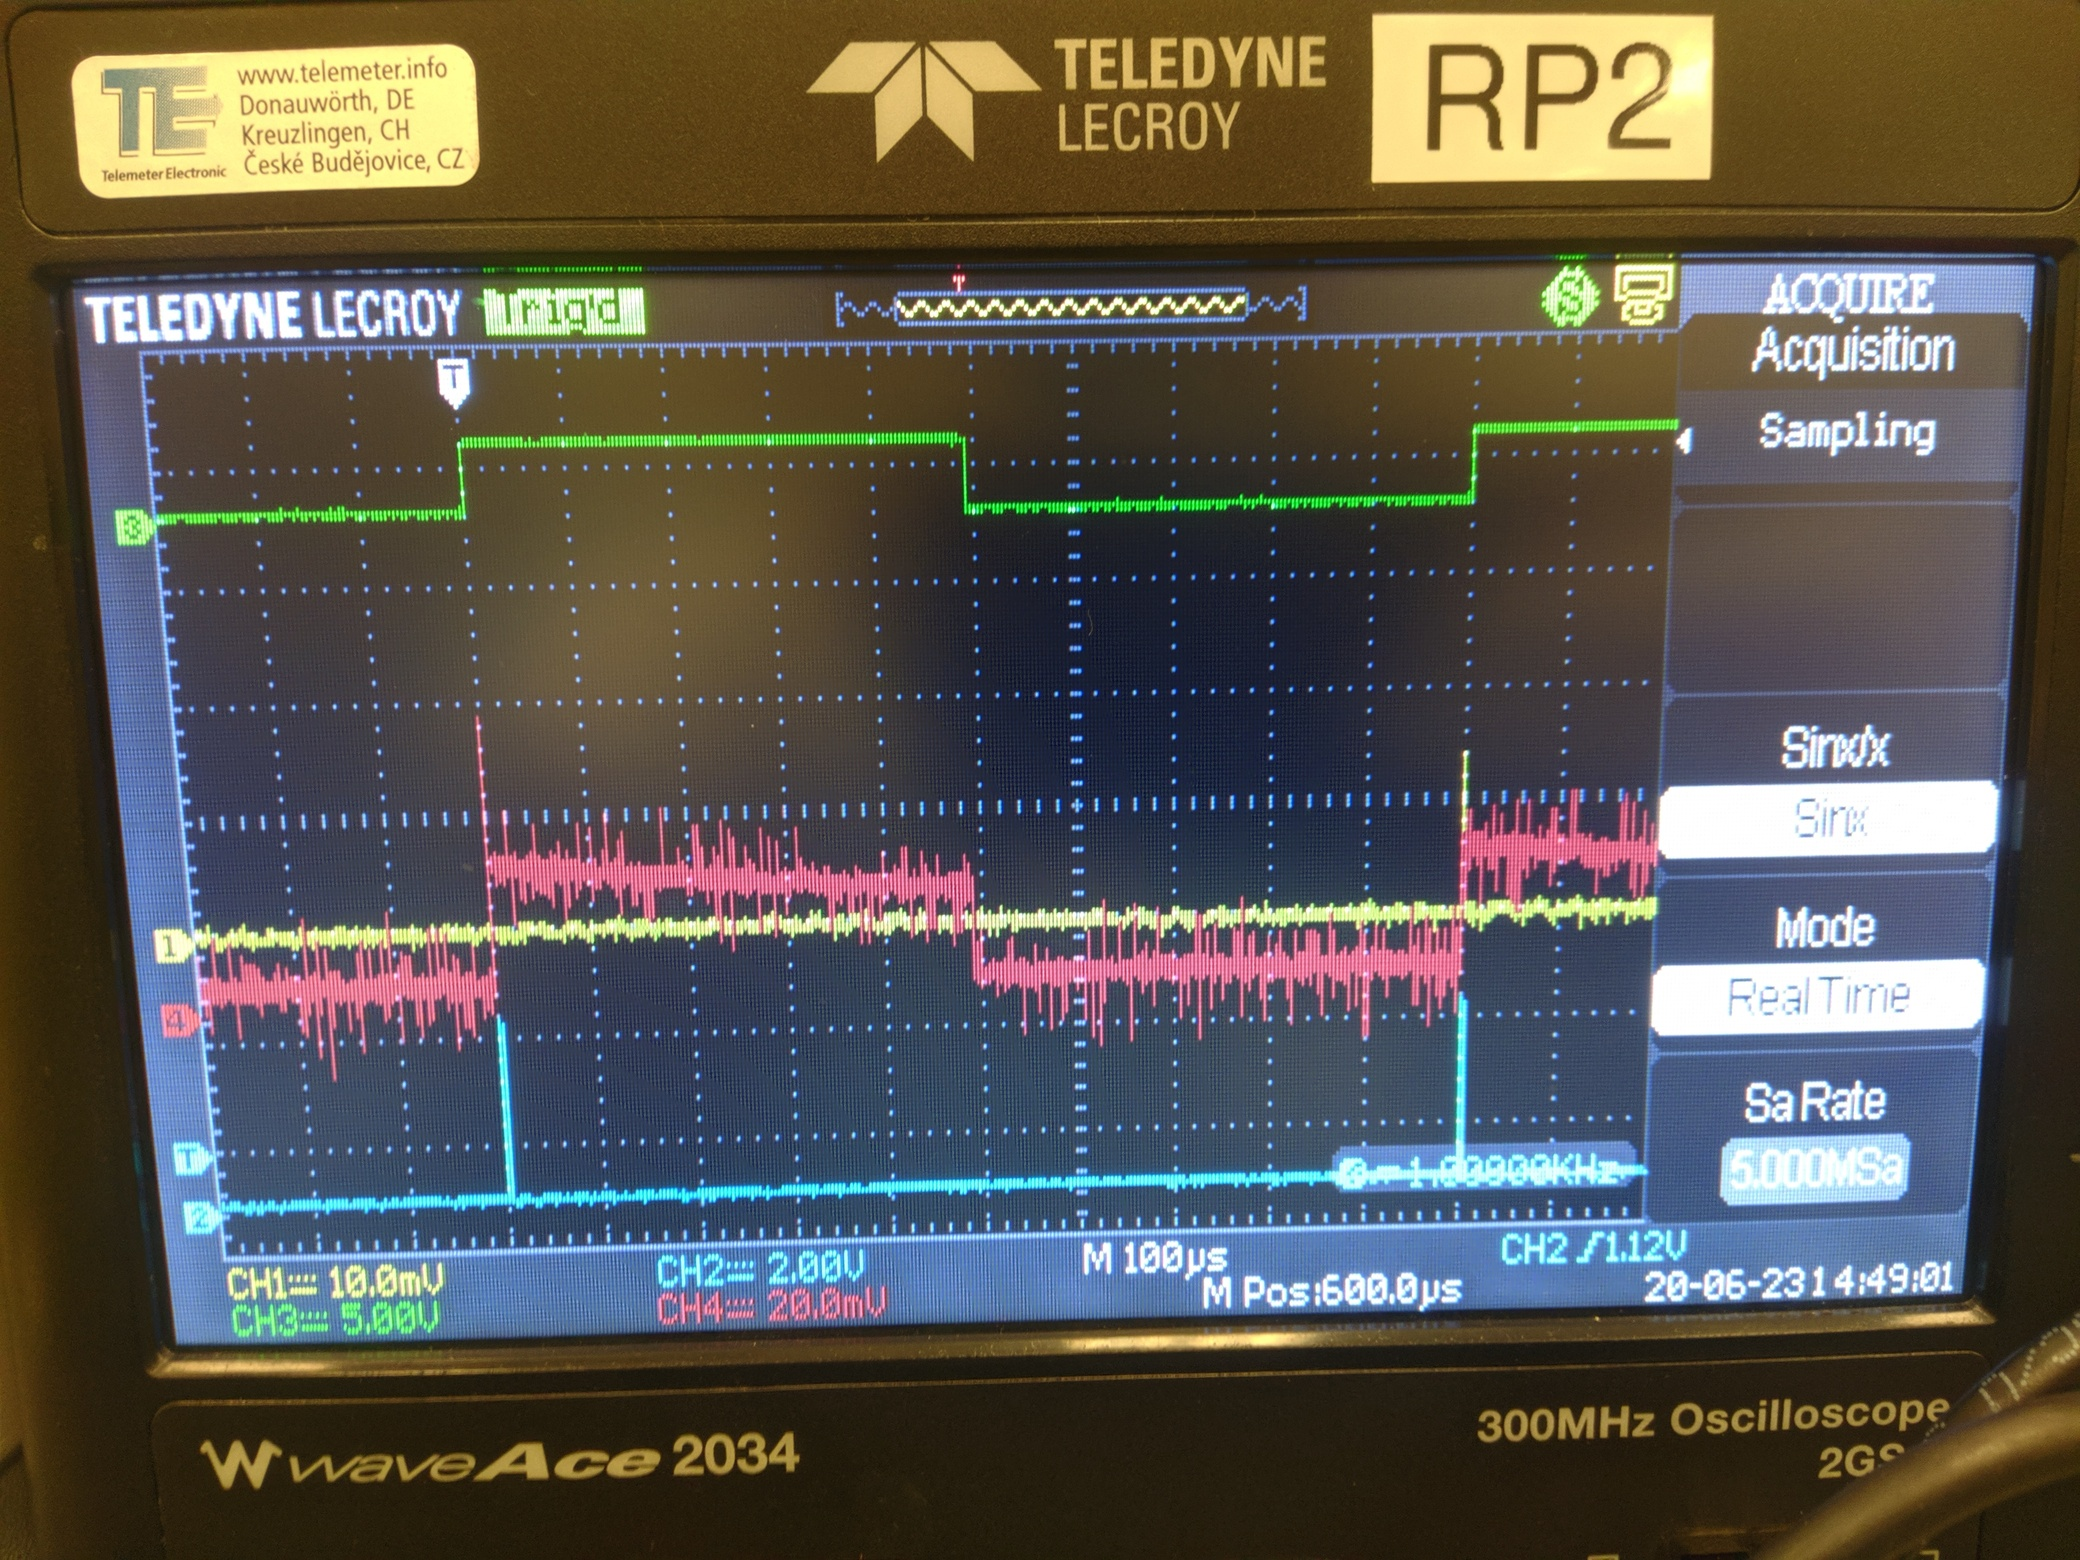
\includegraphics[width=\textwidth]{./images/config-width-sampling.jpg}
        \caption{Oscilloscope set on sampling to show the noise.}
        \label{fig:config-width-sampling}
    \end{subfigure}
    \begin{subfigure}{0.45\textwidth}
        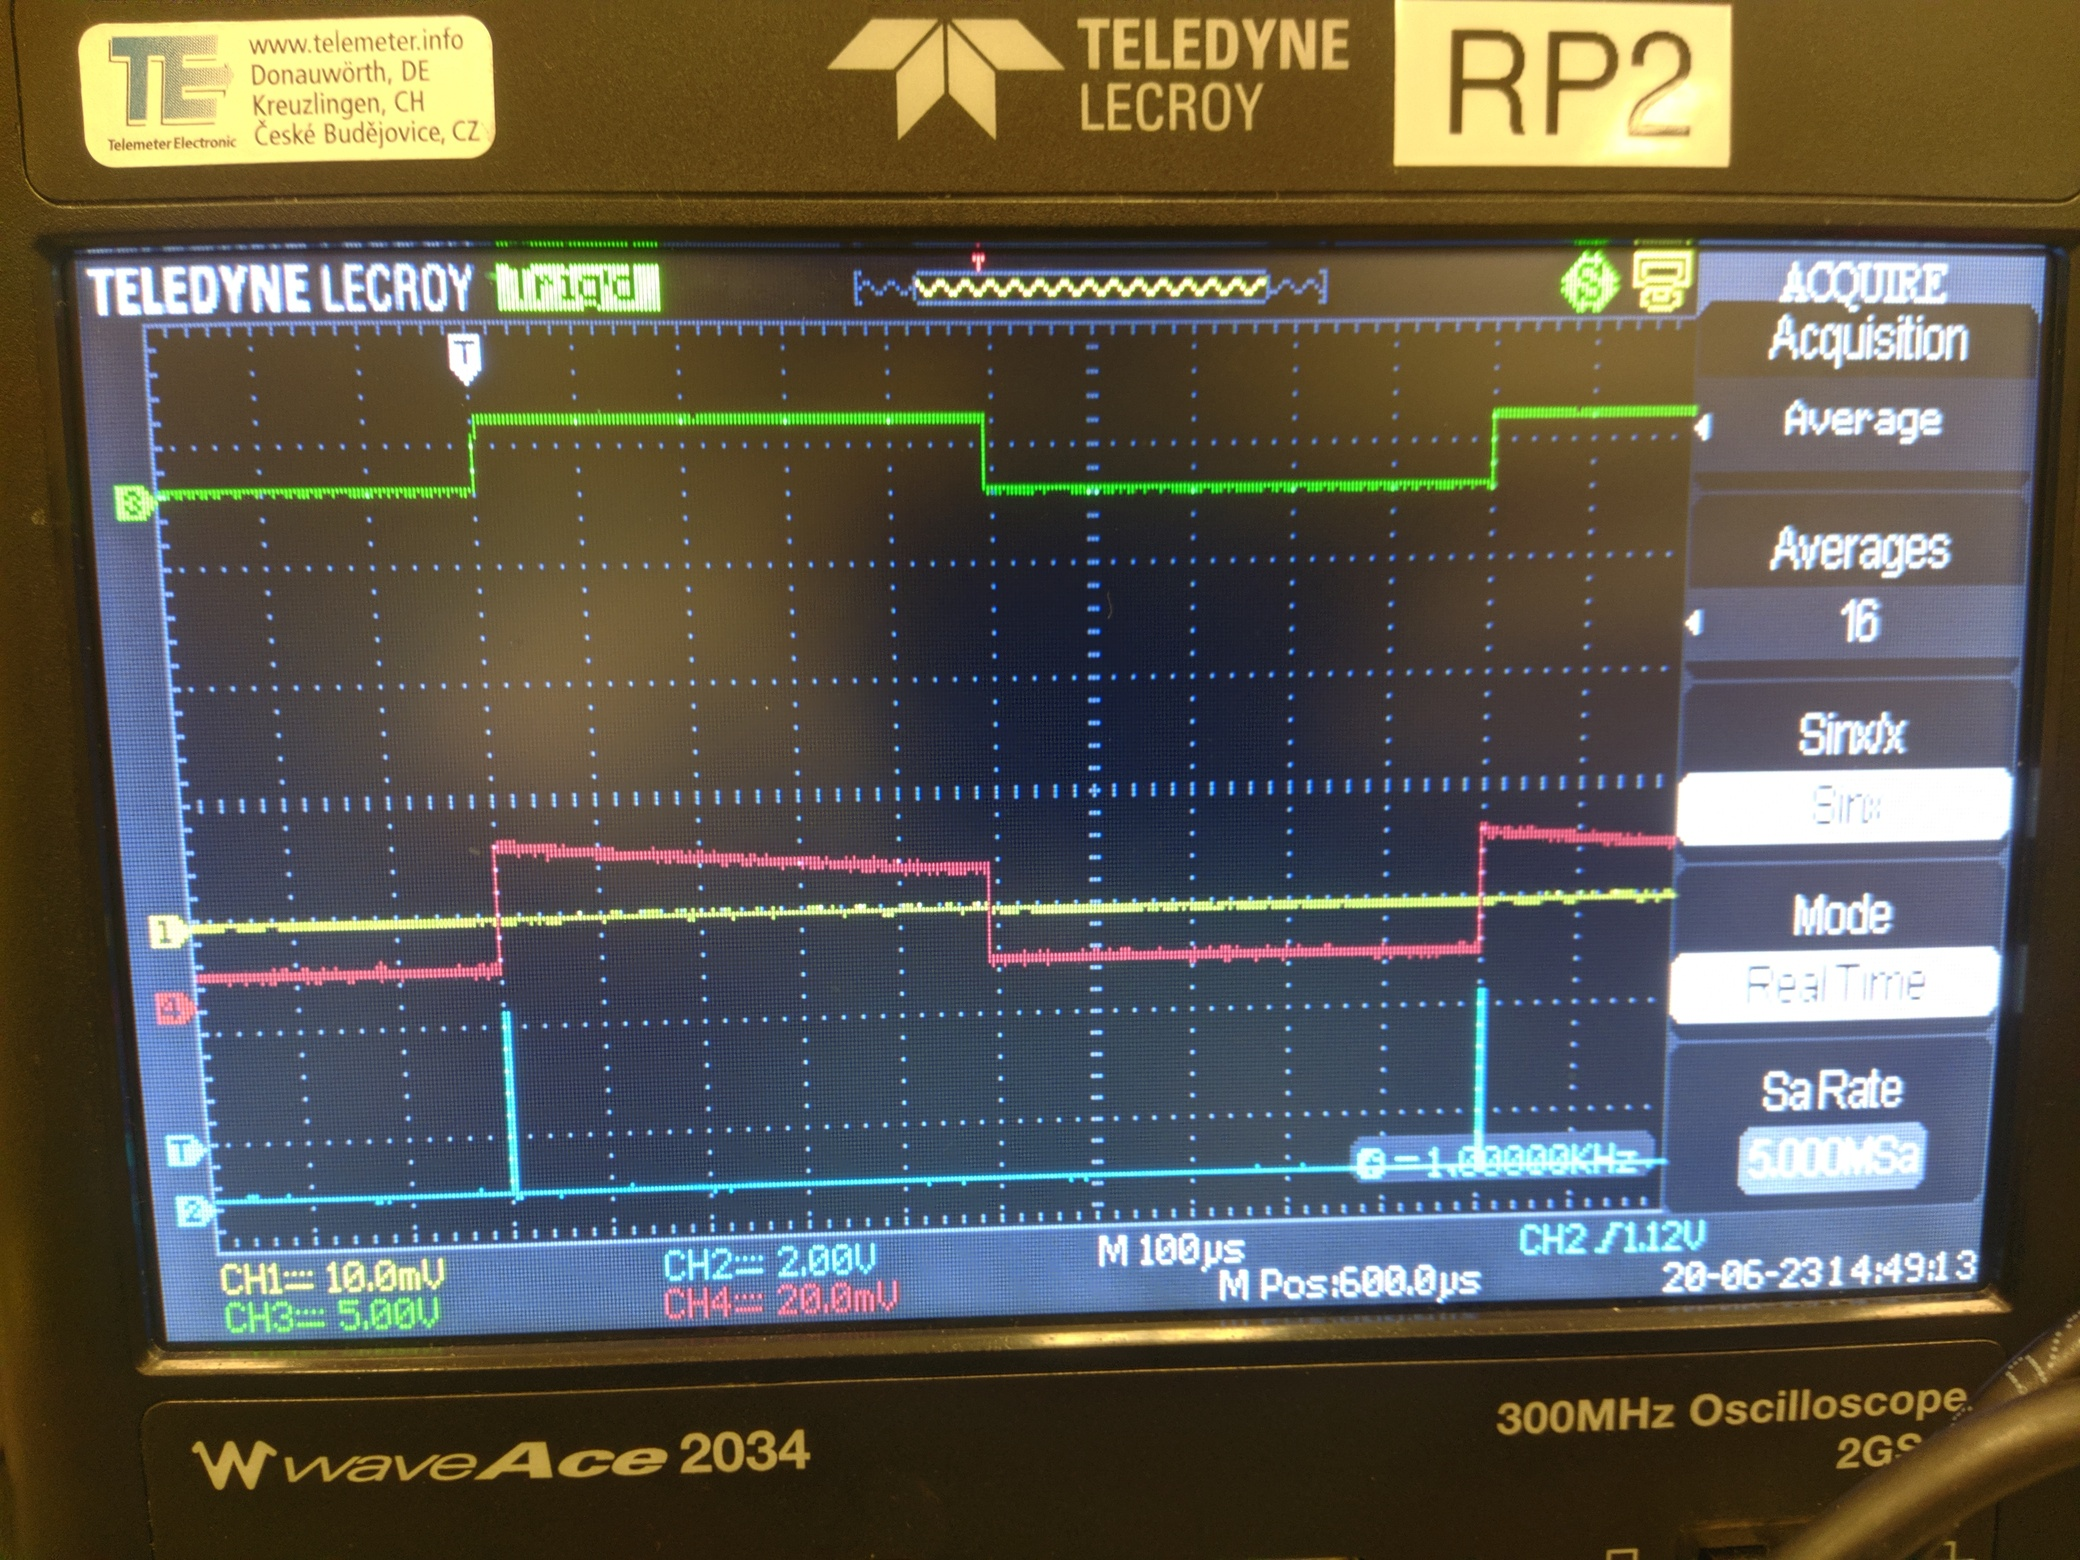
\includegraphics[width=\textwidth]{./images/config-width-averaging.jpg}
        \caption{Oscilloscope on averaging shows the decay nicely.}
        \label{fig:config-width-averaging}
    \end{subfigure}
    \caption{Here you can see the oscilloscope as the pulse delay has been adjusted. Once again connections are the same as in \cref{fig:sample-hold-osci}.}
    \label{fig:config-width}
\end{figure}

Now you need to connect the S\&H SIG OUT to the NI-6002 port AI0 and AI GND.
Then just connect the device to a the computer and start up the software.

\section{Software}
Instructions on how to install and run the software are in the README file.
The software is mostly web based and written in Python.
Once you start the server you can visit the web page on port 8050 (you type `\lstinline{<ip>:8050}` in the url bar in the browser where \lstinline{<ip>} is the ip address of the computer).
You should get a website with 4 tabs, the two middle ones may be disabled and a warning may pop up on load.
The rightmost tab is the help tab, there you can find some information on how to use the software.
The technical documentation of the code itself is distributed with the code itself, here I will provide some notes about the data analysis itself.

\subsection{Data Analysis Description}
Once the data acquisition starts a thread is created which continuously gathers data from the NI-6002 as fast as possible.
The data here is the output of the S\&H but it looks differently then it does in the oscilloscope, visible in \cref{fig:soft-raw-data}.
Here a superposition with a sine wave is clearly visible (or maybe a different function, depending on the lab, in our case the wave is a 50 \si{\hertz} sine so it's quite likely it's due to the plugs).

\begin{figure}[H]
    \centering
    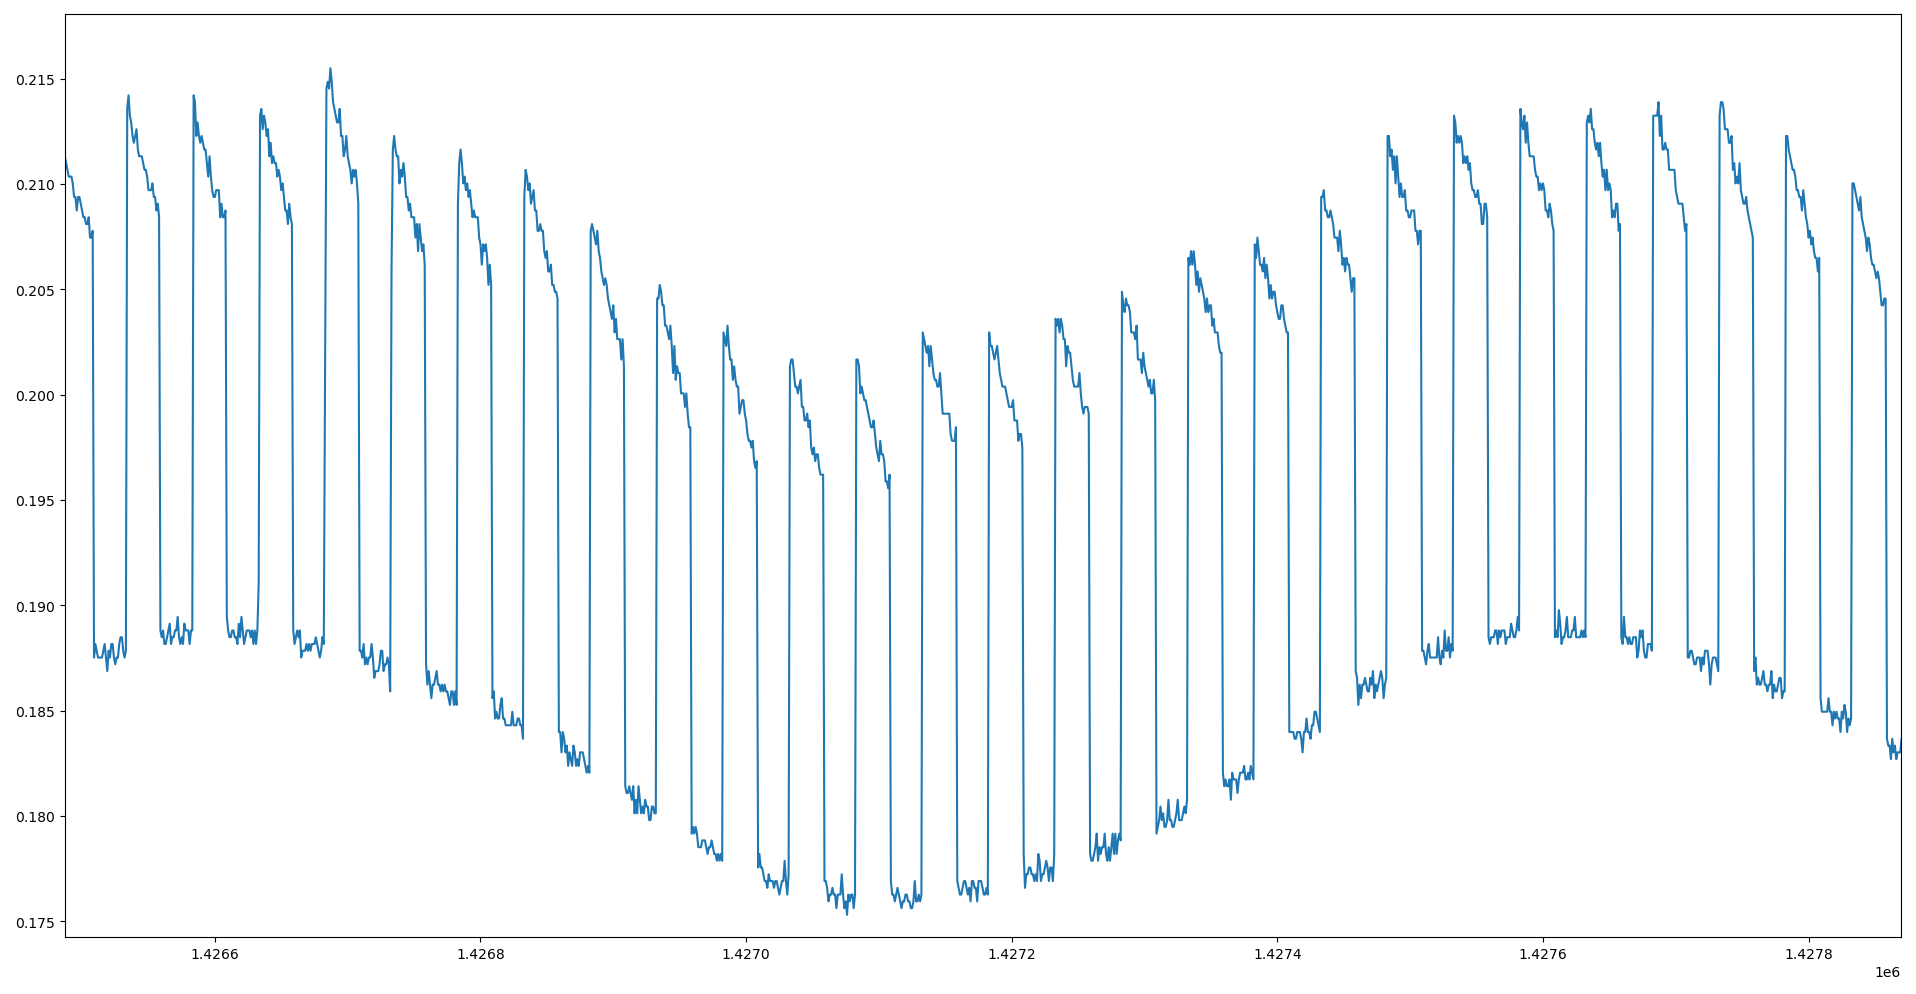
\includegraphics[width=0.9\textwidth]{./images/soft-raw-data.png}
    \caption{Raw data captured by the NI-6002.}
    \label{fig:soft-raw-data}
\end{figure}

First of all when section is written it refers to a group of datapoints between two sharp edges, it corresponds to when the TRIG IN signal on the S\&H is either on or off, but not currently changing.
Sections alternate between up and down sections, up sections also having a slope.
The software always remembers data about the last two sections.

When the software gets a new datapoint, first of all it calculates a value called `diff` in the code, this is the difference between the new datapoint and the last one.
Then it is checked if the absolute value of `diff` exceeds a parameter caled Edgde Detection Threshold (EDT).

If so, then it checks if `diff` is positive or negative.
If it is negative, that means that that an up section must have just ended and a down section should have been before it.
To verify that it checks whether the average of the last section is greater than the average of the previous last section.
If that is the case then it proceeds to get a voltage difference between the two sections and saves it.

It gets the voltage difference by first removing the outliers from each section (this is important for when some of the datapoints land on the edge between sections).
Then it gets the averages of each section and also the average slope of the up section.
It then moves the up section average by the average slope to get the actual peak.
Then it gets the difference between the peak and the average of the down section.

Now going back, if the averages of the two last sections do not match up, it prints a warning message to let the user know that there must have been some anomaly, this feedback can be used to adjust various parameters.
Going another step back, if `diff` is positive, nothing is done.

\begin{figure}[H]
    \centering
    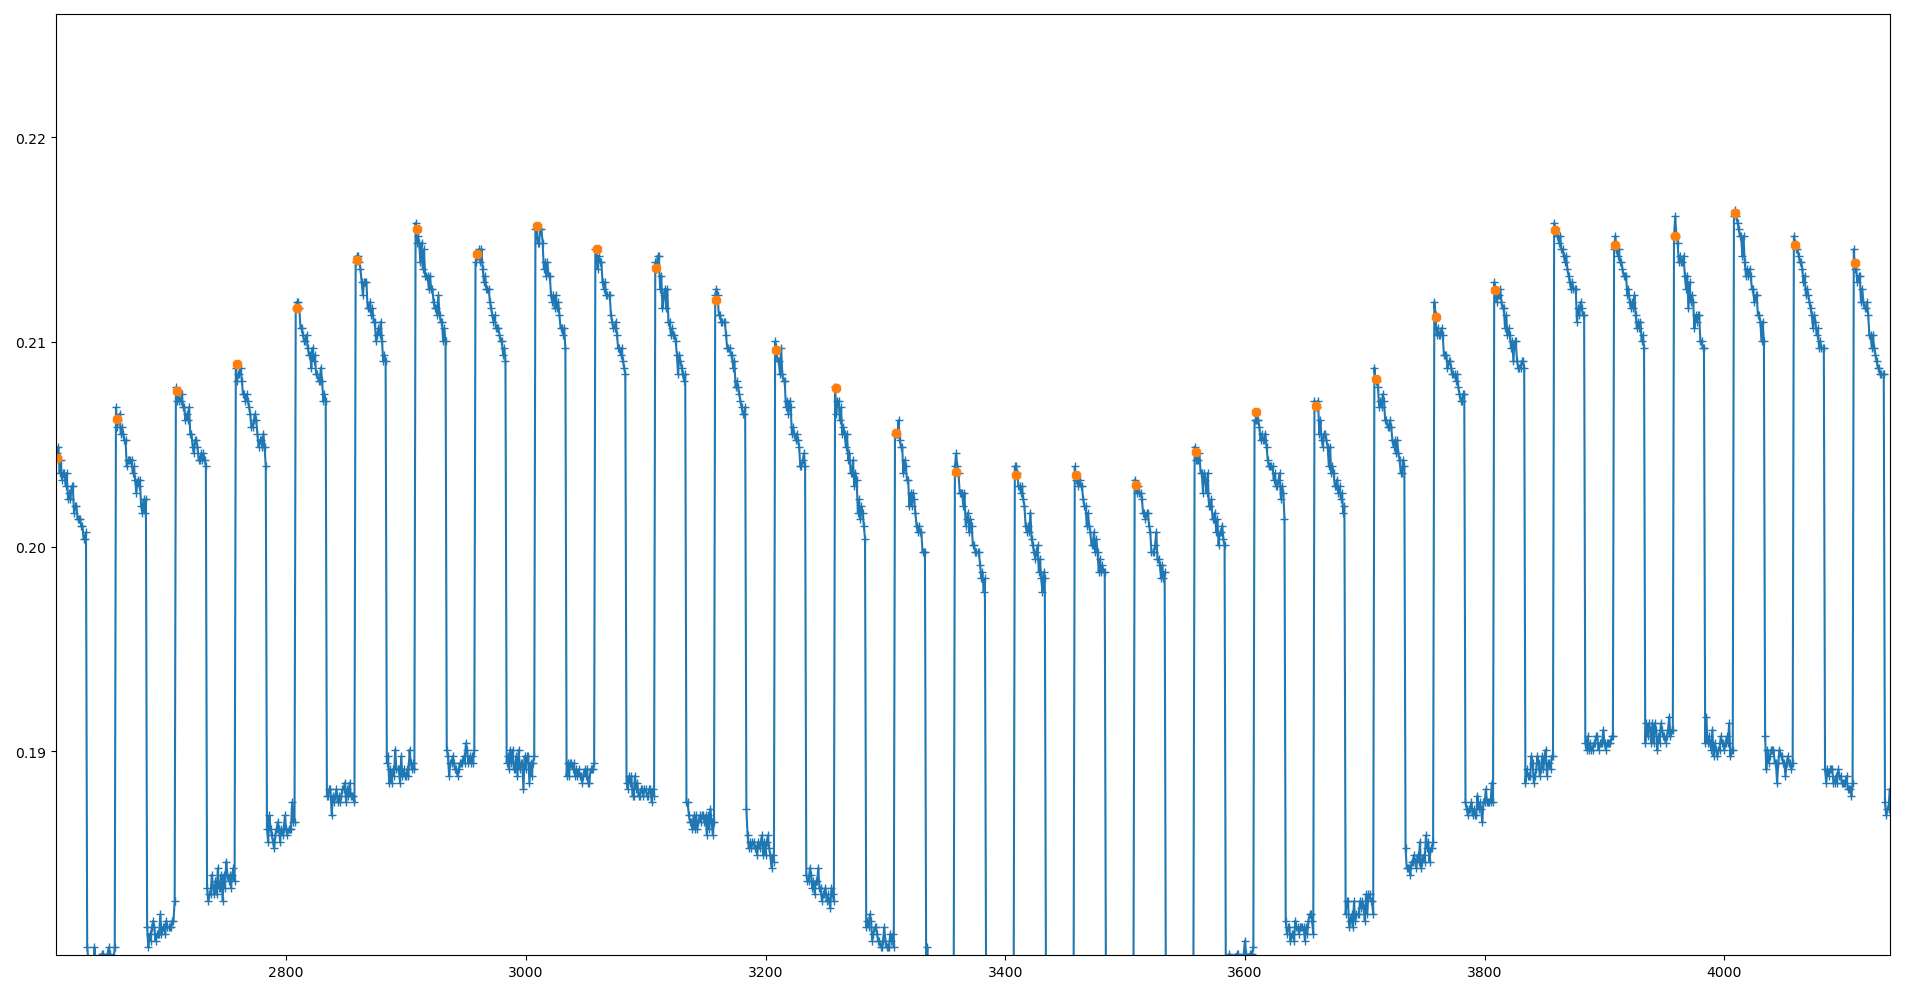
\includegraphics[width=0.9\textwidth]{./images/soft-spike-est.png}
    \caption{Showcase of the precision of peak estimation.}
    \label{fig:soft-spike-est}
\end{figure}

However there is another condition, if the absolute value of `diff` is bigger than Edge Detection Threshold and there are some values gathered in the last section, then it forgets the current previous last section and moves the current last section in its place.
It also resets the values for the last section.

Lastly only if the absolute value of `diff` is lower than EDT, it adds the datapoint to the current section.
This is also important when datapoints land on the edge between sections.

In case a programmer wants to look at the code instead, all of this is in the `\lstinline{handle_processing}` method of `\lstinline{DataAnalyser}`

\subsection{Data Analysis Artifacts}
It was mentioned that the captured data is a superposition of the data we want and an underlying function (in our case a sine wave).
This underlying function does affect the processed data (peak voltages).
Whenever the gradient of the function is positive, the peak voltages are increased by some magnitude and the other way around.
This is caused by how the processing works and can be seen in \cref{fig:soft-ys-pys-corr}.

\begin{figure}[H]
    \centering
    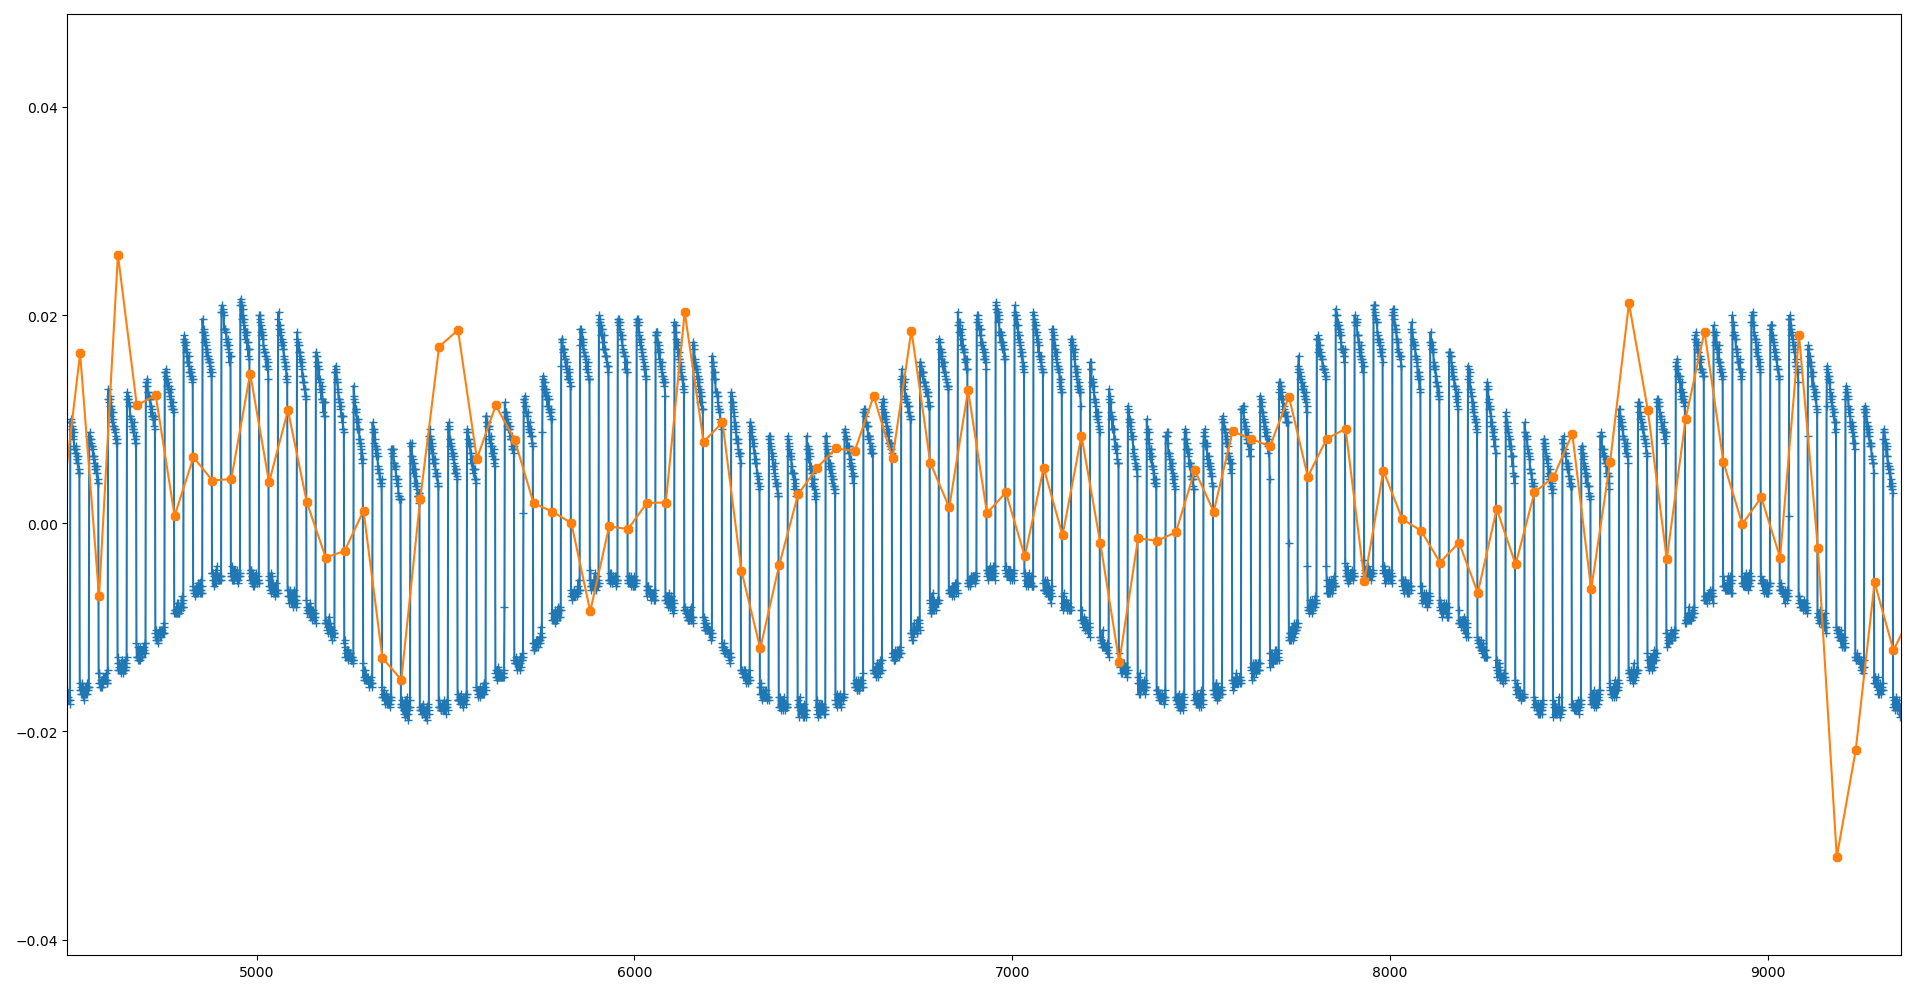
\includegraphics[width=0.9\textwidth]{./images/soft-ys-pys-corr.png}
    \caption{A comparison of raw data peak voltages, both normalized and adjusted so that they can be easily compared.}
    \label{fig:soft-ys-pys-corr}
\end{figure}

\vspace{10em}
\appendix

\section{S\&H Schematic}\label{sec:sample-hold-schema}
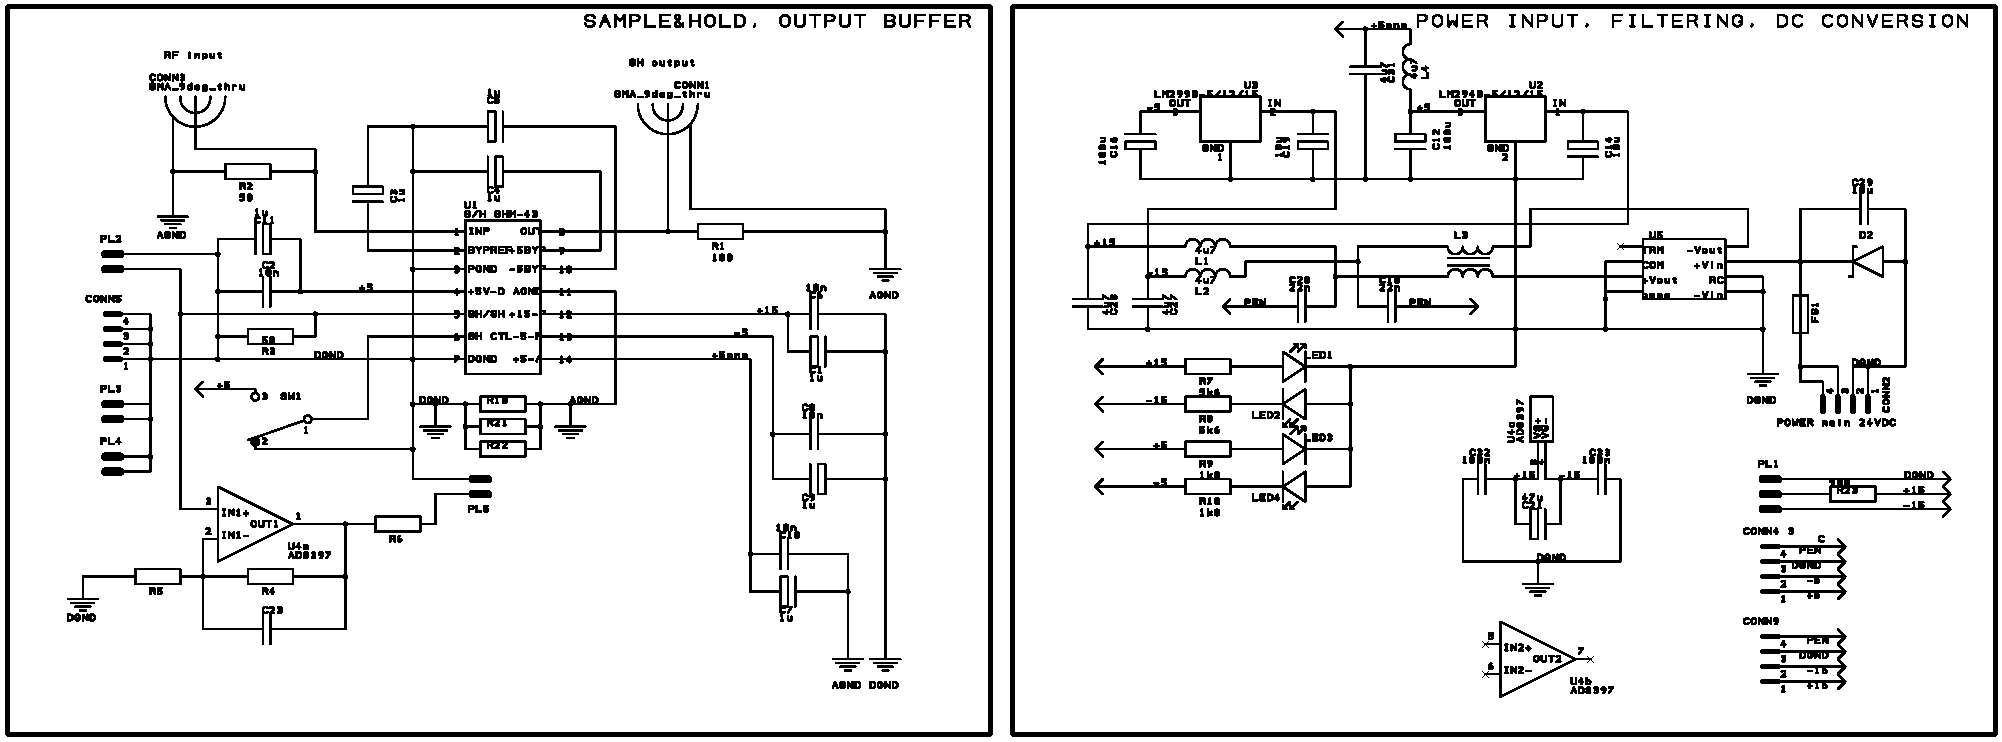
\includegraphics[width=\textwidth]{./appendices/S&H_Scheme.pdf}

\end{document}
